\documentclass[a4paper,10pt]{article}
\usepackage{graphicx}

\usepackage[utf8]{inputenc}
\usepackage[portuguese,brazil]{babel}
\usepackage[T1]{fontenc}

\usepackage{indentfirst}
\usepackage{url}

\usepackage{float}
\floatstyle{boxed}
\restylefloat{figure}

\begin{document}


\begin{titlepage}

\begin{minipage}{0.2\linewidth}
 
\includegraphics[]{./minerva.png}
\end{minipage}
\begin{minipage}{0.8\linewidth}
 \textbf{Universidade Federal do Rio de Janeiro}\\
 Instituto de Matemática\\
 Departamento de Ciência da Computação\\
 \rule{0.8\linewidth}{0.5mm}\\
 Rio de Janeiro, RJ - Brasil
\end{minipage}

\begin{center}

\vspace{2cm}

\Large
Trabalho de Simulação: Implementação e análise de um simulador.

\vspace{1cm}

\large

Bruno C. Buss

\vspace{0.5cm}

Felipe P. Martinez

\vspace{0.5cm}

Rafael O. Lopes

\vspace{0.5cm}

Yanko G. Oliveira

\vspace{1.5cm}

Relatório gerado em \today

\normalsize
\end{center}

\vfill

\begin{flushright}
Disciplina: Avaliação e Desempenho 2010/2\\
Professor: Paulo Henrique de Aguiar Rodrigues\\
\end{flushright}

\vspace{2cm}

\end{titlepage}

\pagebreak


\begin{center}
\vspace{1cm}

\large

\_\_\_\_\_\_\_\_\_\_\_\_\_\_\_\_\_\_\_\_\_\_\_\_\_\_\_\_\_\_\_\_\_\_\_\_\_\_\_\\
Bruno C. Buss

\vspace{0.5cm}

\_\_\_\_\_\_\_\_\_\_\_\_\_\_\_\_\_\_\_\_\_\_\_\_\_\_\_\_\_\_\_\_\_\_\_\_\_\_\_\\
Felipe P. Martinez

\vspace{0.5cm}

\_\_\_\_\_\_\_\_\_\_\_\_\_\_\_\_\_\_\_\_\_\_\_\_\_\_\_\_\_\_\_\_\_\_\_\_\_\_\_\\
Rafael O. Lopes

\vspace{0.5cm}

\_\_\_\_\_\_\_\_\_\_\_\_\_\_\_\_\_\_\_\_\_\_\_\_\_\_\_\_\_\_\_\_\_\_\_\_\_\_\_\\
Yanko G. Oliveira

\vspace{0.5cm}

\vspace{1cm}

\normalsize
\end{center}

Os membros do grupo aqui atestam que tiveram participação ativa e direta em todas as fases do trabalho:
\begin{itemize}
	\item Projeto, construção e documentação do simulador.
	\item Análise dos resultados e elaboração do relatório.
\end{itemize}


\pagebreak



\tableofcontents
\pagebreak

\listoffigures
\pagebreak

\section{Introdução}
\subsection{Funcionamento Geral do Simulador}

    O simulador é executado por linha de comando (comando padrão: "./cmulator"). Este aguarda diversos parâmetros que podem ser passados pela linha de comando ou, caso isso não seja feito, são pedidos em tempo de execução. Tais parâmetros são:

\begin {itemize}
\item \textbf{Modo:} O usuário escolhe qual o parâmetro de execução da simulação, se será replicativo ou batch. Na linha de comando: \emph{--modo} ou \emph{-m}. Opções possíveis: \emph{"Batch"} ou \emph{"Replicativo"};

\item \textbf{Quantidade de rodadas:} O usuário decide a quantidade de rodadas; esta deve ser superior a 10, pois apenas assim temos um valor assintótico na tabela t-student para o cálculo do intervalo de confiança. Na linha de comando: \emph{--n\_rodadas} ou \emph{-n}. Opções possíveis: números inteiros;

\item \textbf{Tamanho da rodada:} Determina a quantidade de fregueses típicos em cada rodada. Na linha de comando: \emph{--t\_rodada} ou \emph{-r}. Opções possíveis: números inteiros;

\item \textbf{Tamanho da fase transiente:} Determina a quantidade de fregueses típicos a serem considerados pertencentes à fase transiente, de forma a considerarmos apenas dados coletados após o sistema estar em equilíbrio. Na linha de comando: \emph{--t\_transiente} ou \emph{-t}. Opções possíveis: números inteiros;

\item \textbf{Tipo da fila 1:} O tipo da fila pode ser FCFS(fila), ou LCFS(pilha). Na linha de comando: \emph{--fila\_1} ou \emph{-1}. Opções possíveis: \emph{"FCFS"} ou \emph{"LCFS"};

\item \textbf{Tipo da fila 2:} Assim como a fila 1, a fila 2 pode ser FCFS ou LCFS. Na linha de comando: \emph{--fila\_2} ou \emph{-2}. Opções possíveis: \emph{"FCFS"} ou \emph{"LCFS"};

\item \textbf{Taxa $\lambda$:} Determina a taxa de chegada de chegada de fregueses no sistema. Na linha de comando: \emph{--tx\_lambda} ou \emph{-l}. Opções possíveis: números reais;

\item \textbf{Taxa $\mu$:} Determina a taxa de serviço de fregueses no sistema. Na linha de comando: \emph{--tx\_mi} ou \emph{-m}. Opções possíveis: números reais.
\end {itemize}

    Além desses parâmetros que são obrigatórios para a execução do simulador, existem outros parâmetros opcionais, a serem passados pela linha de comando:

\begin {itemize}
\item \textbf{Semente para gerador de chegadas:} semente utilizada para o gerador de números pseudo-aleatórios responsável por gerar os tempos de chegada. Na linha de comando: \emph{--seed\_gerador\_chegadas} ou \emph{-c}. Opções possíveis: números reais;

\item \textbf{Semente para gerador de tempos de serviço:} semente utilizada para o gerador de números pseudo-aleatórios responsável por gerar os tempos de serviço. Na linha de comando: \emph{--seed\_gerador\_tempo\_servico} ou \emph{-x}. Opções possíveis: números reais;

\item \textbf{Sobre:} imprime informações sobre o simulador e seus autores. Na linha de comando: \emph{--sobre} ou \emph{-s}. Não recebe parâmetros;

\item \textbf{Ajuda:} imprime todos os comandos possíveis e suas descrições. Na linha de comando: \emph{--ajuda} ou \emph{-a}. Não recebe parâmetros;

\item \textbf{Benchmark:} o simulador executa um benchmark para diversos valores de tamanho para a fase transiente. Na linha de comando: \emph{--benchmark} ou \emph{-b}. Não recebe parâmetros;

\item \textbf{Determinístico:} indica ao simulador que os geradores de chegada e de servico devem atuar em modo deterministico, para fins de verificação. Na linha de comando: \emph{--deterministico} ou \emph{-d}. Não recebe parâmetros;

\item \textbf{Modo de coloração:} Neste modo é ignorada a coloração da rodada à qual os fregueses pertencem (por padrão, o simulador roda com coloração ligada). Na linha de comando: \emph{--modo\_coloracao} ou \emph{-o}. Não recebe parâmetros;


\item \textbf{Modo verborrágico:} roda o simulador imprimindo diferentes níveis de detalhe sobre as operações sendo executadas internamente. Na linha de comando: \emph{--verbose} ou \emph{-v} Opções: 0 (apresenta apenas os intervalos de confiança), 1 (o mesmo que o anterior, mais os dados finais de cada rodada) ou 2 (modo 1 mais dados de cada evento que ocorre na rodada);
\end {itemize}

    Após a entrada de parâmetros, o simulador se inicia. Este utiliza eventos discretos, mas tempo contínuo, logo, os eventos acontecem em instantes de tempo com valores numéricos reais. A cada rodada, o simulador fica em loop aguardando eventos acontecerem. O loop se encerra quando a quantidade de fregueses determinada pelo parâmetro \emph{"tamanho da rodada"} for servida. Os eventos que acontecem são:

\begin {itemize}
\item \textbf{Chegada de um freguês na fila 1:} Um freguês chega e é inserido na fila 1, de acordo com a disciplina de atendimento escolhida - caso seja FCFS, o mesmo é inserido no final e, caso seja LCFS, é adicionado no início.

\item \textbf{Término do serviço do freguês no servidor:} No momento em que um freguês termina seu atendimento no servidor, é verificado qual sua fila original. Caso seja a fila 1,
ele é movido para a fila 2 (sempre respeitando a disciplina de atendimento). Se o freguês veio da fila 2, dados estatísticos são coletados e o mesmo é retirado do sistema.
\end {itemize}

    Após a tratar o evento ocorrido, verifica-se se o servidor está vazio. Caso esteja, é inserido no servidor um freguês, de acordo com as regras determinadas; neste caso, dando prioridade aos fregueses da fila 1 e sendo os da fila 2 servidos apenas quando a primeira estiver vazia.

    Após a execução de todas as rodadas, os dados estatísticos coletados são analisados e é calculado o intervalo de confiança para cada variável aleatória. O programa se encerra imprimindo na tela a linha de comando com todos os parâmetros utilizados (mesmo que estes tenham sido entrados em tempo de execução), incluindo as sementes geradoras para, caso seja desejado, executar mais uma vez a exata mesma rotina.

\subsection{Linguagem de Programação Utilizada}

    Foi utilizada a linguagem de programação C++. O compilador utilizado para desenvolver o sistema foi o GCC 4.4, presente em qualquer distribuição atualizada do Linux, de forma que o sistema pode ser compilado em qualquer ambiente que possua o GCC 4.4 ou superior instalado.

\emph{Nota: O sistema utiliza algumas extensões da biblioteca padrão c que podem não estar presentes nos ambientes MinGW para plataformas Windows. Devido a isto o programa foi testado em sistemas Ubuntu de 32 e 64 bits.}

    Um dos principais fatores para escolha da linguagem foi a possibilidade de lidar com orientação a objetos, tornando o código mais claro e de melhor entendimento. Além disso como o simulador é um software de uso intensivo da CPU, uma linguagem compilada para assembly da máquina e sem camadas adicionais (como máquinas virtuais) era uma boa escolha para o desenvolvimento visando a performance. Um último fator foi o fato de que C++ é a linguagem com que os membros do grupo estão melhor familiarizados, proporcionando uma maior facilidade na hora da implementação.

    O programa foi completamente desenvolvido e testado em ambiente Linux.

\subsection{Estruturas Internas Utilizadas}

    Todo o código do simulador está comentado e foi documentado utilizando a ferramenta \emph{DoxyGen}, estando a documentação gerada anexa. Nesta seção, faremos uma breve análise da implementação e estruturas utilizadas.

    Todas as estruturas do simulador estão no namespace \emph{TrabalhoAD} permitindo não só maior organização do código do próprio trabalho mas também caso eventualmente este seja utilizado juntamente a outras aplicações. Nele há as classes \emph{Evento, DistExponencial, Fregues} e \emph{Simulador}, as structs \emph{AmostragemFila} e \emph{ResultadosConsolidados}, além dos operadores sobrecarregados \emph{$>$} e \emph{$>=$} e das enumerações \emph{ETipo} e \emph{TipoFila}.

    Os operadores sobrecarregados são responsáveis por comparar dois eventos do simulador, sendo o maior aquele com o tempo em que ocorreu de valor mais alto. Os enums \emph{ETipo} e \emph{TipoFila} listam, respectivamente, os tipos de evento possíveis (se um novo freguês chegou ao sistema, ou se seu serviço terminou de ser executado) e o regime de serviço das filas (FCFS ou LCFS).

    Descrição breve das classes:

\begin {itemize}
\item \textbf{class Evento:} representa um evento ocorrido no sistema, descrevendo seu tipo o tempo em que ocorrerá;

\item \textbf{class DistExponencial:} responsável pelo gerador pseudo-aleatório de tempos entre chegadas exponencialmente distribuídas. O método de geração é através da função inversa a PDF da distribuição exponencial. Além disso, a semente inicial é guardada, para que a simulação possa ser repetida de forma precisa;

\item \textbf{class Fregues:} representa um freguês que chegou durante a simulação. É a responsável por gravar todos os dados da simulação (o tempo em que entrou e saiu das filas, o tempo de espera, qual fila está atualmente, a qual rodada pertence etc);

\item \textbf{class Simulador:} responsável por executar a simulação propriamente dita, coletar e armazenar os resultados de cada rodada e apresentar o resultado final da simulação.
\end {itemize}

    Além destas, temos os structs:

\begin {itemize}
\item \textbf{struct AmostragemFila:} unifica todos os dados de uma determinada fila. Nela constam as quantidades de pessoas na fila, a soma dos tempo de espera, no servidor etc e seus quadrados, para posterior análise estatística;

\item \textbf{struct ResultadosConsolidados:} reúne todos os dados coletados das \emph{duas} filas (através de duas \emph{AmostragemFila}) e da quantidade de amostras analisadas.
\end {itemize}


% Aqui comentamos sobre as classes do projeto, e alguns detalhes, como a utilização do rand do linux, ou de
\subsection{Implementação da Lista de Eventos}

	Para a implementação da lista de eventos, foi utilizada uma heap de mínimo. Como o simulador é orientado a eventos, utilizando esta estrutura
	de dados podemos inserir novos eventos em $O(log n)$ e identificar o próximo evento a ser tratado em $O(1)$.

	Existem dois tipos de eventos no sistema:
	\begin{itemize}
		\item Nova chegada
		\item Término de serviço
	\end{itemize}

	Durante todo o funcionamento do simulador, existem duas invariantes:
	\begin{itemize}
		\item Sempre existe um evento do tipo "Nova chegada" na fila de eventos.
		\item Sempre que existir ao menos um freguês no sistema, existe um evento do tipo "Término de serviço" na fila de eventos.
	\end{itemize}

	Estas duas invariantes são garantidas da seguinte forma:
	\begin{itemize}
		\item Quando um evento do tipo "Nova chegada" é tratado e removido da fila, outro evento é inserido imediatamente, agendando a próxima chegada ao sistema.
		\item Quando um evento do tipo "Término de serviço" é tratado, caso ainda exista alguém no sistema, fila 1 ou fila 2, respeitando as respectivas prioridades, então um freguês é movido ao servidor e um novo evento do tipo "Término de serviço" é gerado e adicionado à lista de eventos.
    \end{itemize}

\subsection{Geração das Variáveis Aleatórias}
% Aqui dizemos as variáveis aleatórias que temos, e como elas são calculadas(mencionar a inversa da exponencial etc)
% Buss falará aqui também da srand.

	Para gerar o tempo de execução das variáveis aleatórias, utilizamos a função inversa da CDF da exponencial. A transformação foi feita da seguinte forma:

    $ y = 1 - e^{-\lambda x} $

    $ 1 - y  = e^{-\lambda x} $

    $ -\lambda x = log (1 - y) $

    $ x = -{log(1 - y)} / \lambda $

	Portanto a inversa da CDF da exponencial é $ x = -{log(1 - y)} / \lambda $, onde y é a probabilidade do evento acontecer.

	Cada evento tem uma determinada probabilidade, escolhida de forma aleatória. No momento em que um evento é gerado, é indicada uma probabilidade e a taxa $\lambda$. Assim, sabemos o tempo em que tal evento ocorre.

	Um detalhe importante, é que foi utilizado um geradores de números pseudo-aleatórios diferentes do padrão \emph{rand} e \emph{srand} da biblioteca padrão C. Os geradores utilizados são considerados \emph{extensões GNU} e por isso estão presente em todos os sistema Linux modernos.

	Os geradores utilizados foram os \emph{drand48\_r\(\)} e \emph{srand48\_r\(\)}, o gerador de números e o inicializador do gerador respectivamente.

	Esta escolha foi feita principalmente por 3 razões técnicas:
	\begin{itemize}
	\item Este gerador de números aleatórios utiliza um estado de 48 bits e não 32 bits como o \emph{rand} padrão. Além disso, a entropia dos bits menos significativos é maior no \emph{drand48} do que no \emph{rand}. Para a maioria dos aplicativos, isto não faz muita diferença, mas como estamos trabalhando com amostragens é importante este aspecto.

	\item O \emph{drand48} retorna um \emph{double} entre $0.0$ e $0.99...$ (ou seja, entre zero e um, aberto no um). Além de ser uma comodidade, pois precisamos de um número real neste intervalo para passarmos a inversa da CDF da exponencial existe um outro ponto matemático pouco conhecido. Ao pegar o número gerado pelo \emph{rand} e fazer módulo um número N e após isso dividir este resultado por N para obter um número entre zero e um (aberto no um), quebra-se a propriedade da distribuição uniforme do \emph{rand} e assim estragando a qualidade dos números gerados.

	\item O item final é que o \emph{drand48} é uma função reentrante, o que permite que o código seja portável para multi-thread sem que um gerador altere o estado de outro gerador de outra thread. Isto é muito importante caso queiramos implementar capacidade de multi-threading no simulador.
	\end{itemize}

\subsection{Coleta de Estatísticas}
% Falamos sobre a coleta de estatísticas e cálculo delas(Variância e IC).

    A coleta de estatísticas é feita sempre quando o freguês, advindo da fila 2, termina seu atendimento no servidor. Neste momento, é verificado se o freguês pertence à rodada atual. Caso ele não pertença, seus dados são ignorados mas, caso pertença à rodada atual, suas estatísticas são coletadas: seu tempo de execução após estar na primeira e segunda fila, seu tempo de espera na primeira e segunda fila (por consequência, temos o tempo total na fila 1 e o tempo total na fila 2), a quantidade de pessoas que já estavam na fila e a quantidade de pessoas no sistema quando ele chega.

    Além de coletar estes dados, no momento em que o freguês que pertence à rodada atual sai do sistema, a quantidade de fregueses executados é incrementada em um, para controlar o fim da rodada em execução.

%falar ainda do calculo das estatisticas
\subsection{Método de análise}

    O simulador foi construído para funcionar de maneira genérica, sendo assim, a única parte fixa é o formato das filas do sistema (fila 1 prioritária sobre fila 2, ambas sendo servidas por um mesmo servidor), enquanto as disciplinas de serviço podem ser escolhidas pelo usuário. Com isso, também foi planejado para aceitar ambos os métodos de análise: Batch e Replicativo.

    No método Batch, diversas rodadas são executadas a partir de uma mesma semente. Desta forma, precisamos estimar a fase transiente apenas uma vez, utilizando apenas um sistema de \emph{"coloração"} para definir quais dados devem ser coletados. Os clientes gerados em uma determinada rodada possuem um identificador da mesma e, quando saem do sistema, apenas são considerados para as estatísticas aqueles pertencentes à rodada atual de simulação. Caso a rodada acabe e ainda haja fregueses na fila, estes permanecem fazendo parte da simulação, mas seus dados não são contados na rodada seguinte. A coloração é implementada utilizando um atributo da classe \emph{Fregues}, que é setado na criação do mesmo.

    No método Replicativo, há uma semente gerada para cada rodada. Sendo assim, há também uma fase transiente para ser estimada. Assim como em uma rodada anterior do método Batch, os fregueses não atendidos que estavam na fila de espera em uma rodada continuam na fila, mas não são computados nas estatísticas da rodada referente. 


% Aqui mencionamos que decidimos testar os dois métodos: Batch e Replicativo. E também falar um pouco sobre eles.
% Acredito que essa seção pode morrer.
%\subsection{Parâmetros Utilizados}
% Essa sub-seção eu peguei do relatório do Jonas. No projeto deles, eles determinaram um valor para alguns parâmetros que nós tomamos como fixos. Creio que isso pode morrer.
\subsection{Tempo Gasto Para Simulação}


\pagebreak

\section{Teste de Correção}

    Para garantirmos a consistência da simulação e dos dados estatísticos coletados, precisamos analisar a corretude dos dados gerados. A abordagem escolhida foi criar um modo determinístico (ativado com a opção \emph{--deterministico} na linha de comando) e, a partir dos resultados gerados por este, fazer as análises que nos mostrariam se o simulador faz a geração de dados corretamente ou não.

    Nossa abordagem envolveu acompanhar fregueses-padrão em diversas situações limítrofes, como por exemplo com apenas uma chegada no sistema, com diversas, com um $\rho$ próximo a 1, maior que 1 etc. para, a partir dos dados gerados por ele, confirmar se seu comportamento era o esperado. Abaixo, seguem estas análises.
\\
\textbf{\emph{MODO BATCH}, filas FCFS}
\\
\\
\emph{Teste:} $\lambda$ = 0.1, $\mu$ = 1
\\
\emph{Linha de comando:}
\\
./cmulator -m batch -n 2 -t 0 -r 3 -1 FCFS -2 FCFS -l 0.1 -u 1.0 -d -v 2 -o
\\
\\
\emph{Resultados:}
\\
\begin{verbatim}
Você já escolheu o modo de simulação: Batch
Você já escolheu a quantidade de rodadas: 2
Você já escolheu o tamanho de cada rodada: 3
Você já escolheu o tamanho da fase transiente: 0
Você já escolheu o tipo da fila 1: FCFS
Você já escolheu o tipo da fila 2: FCFS
Você já escolheu o valor da taxa lambda: 0.100000
Você já escolheu o valor da taxa mi: 1.000000

\end{verbatim}
Para uma instância de execução com estes parâmetros temos o seguinte:

O primeiro freguês chega no sistema no tempo 34.65s, entrando direto na fila 1, que se encontra vazia. Seguindo para o servidor, ele é executado em exatamente 1 segundo, como já previsto: como estamos executando o simulador com $\mu$ = 1, todos os fregueses devem executar em tempo 1/$\mu$, ou seja, 1 segundo. Logo após disso, o freguês segue para a fila 2 e, ao ser servido, leva novamente 1 segundo no servidor.

A segunda chegada no sistema acontece no tempo 44.65s, exatamente 10 segundos depois da primeira chegada. De forma análoga, como estamos no modo determinístico e definimos $\lambda$ em 0.01 esperávamos este resultado. Da mesma forma que o anterior, este freguês leva 1 segundo para ser executado em ambas as vezes, posteriormente saindo do sistema.

O próximo freguês a chegar segue o mesmo padrão de comportamento do outros dois, mantendo-se dentro das expectativas de tempo de chegada e execução.
\\
\\
\emph{Teste:} $\lambda$ = 0.45, $\mu$ = 1
\\
\emph{Linha de comando:}
\\
./cmulator -m batch -n 2 -t 0 -r 3 -1 FCFS -2 FCFS -l 0.45 -u 1.0 -d -v 2 -o
\\
\\
\emph{Resultados:}
\\\begin{verbatim}
Você já escolheu o modo de simulacao: Batch
Você já escolheu a quantidade de rodadas: 2
Você já escolheu o tamanho de cada rodada: 3
Você já escolheu o tamanho da fase transiente: 0
Você já escolheu o tipo da fila 1: FCFS
Você já escolheu o tipo da fila 2: FCFS
Você já escolheu o valor da taxa lambda: 0.450000
Você já escolheu o valor da taxa mi: 1.000000
\end{verbatim}

    Mais uma vez, como $\mu$ é 1, sempre que um freguês passar pelo servidor, vindo da fila 1 ou da fila 2, ele vai levar exatamente 1 segundo para ser executado. Isso de fato acontece para todos os fregueses que são servidos durante toda a execução.

    Para esta taxa de chegada, a situação da primeira rodada é a mesma de quando lambda é \emph{0.1}. Sempre que um freguês chega no servidor, não existe ninguém na fila e ele pode ser executado imediatamente. Assim, a situação é a mesma.
\\
\\
\emph{Teste:} $\lambda$ = 0.6, $\mu$ = 1
\\
\emph{Linha de comando:}
\\
./cmulator -m batch -n 2 -t 0 -r 3 -1 FCFS -2 FCFS -l 0.6 -u 1.0 -d -v 2 -o
\\
\\
\emph{Resultados:}
\\\begin{verbatim}
Você já escolheu o modo de simulacao: Batch
Você já escolheu a quantidade de rodadas: 2
Você já escolheu o tamanho de cada rodada: 3
Você já escolheu o tamanho da fase transiente: 0
Você já escolheu o tipo da fila 1: FCFS
Você já escolheu o tipo da fila 2: FCFS
Você já escolheu o valor da taxa lambda: 0.600000
Você já escolheu o valor da taxa mi: 1.000000
\end{verbatim}

    Aqui, o primeiro freguês chega ao sistema no tempo 2.27s e passa por ele normalmente, terminando sua execução em 3.27s e entrando na fila 2. Logo ele é executado, levando mais 1 segundo e só saindo do servidor, e assim do sistema, no tempo 4.27s.

    O segundo freguês chega ao sistema no tempo 3.93, enquanto o primeiro ainda está sendo servido. Logo, ele tem que esperar na fila 1 0.34 segundos até que o servidor esteja livre, no tempo 4.27s. Em seguida, é executado durante o próximo segundo, entrando na fila 2 no tempo 5.27s. Durante essa execução, um terceiro freguês entra no sistema (no tempo 5.6s), esperando na fila 1 a liberação do servidor.

    Posteriormente, este terceiro freguês sai da fila 1 e entra no servidor para ser executado (tempo 6.27s). Enquanto isso, chega um quarto freguês e é entra na fila 1, sendo executado quando o terceiro freguês terminar de ser servido e entrar na fila 2, 1 segundo depois de sua entrada. Durante a execução deste quarto freguês , um quinto chega no sistema. Nesta hora, tirando uma fotografia do sistema, temos o seguinte: o quinto fregues na fila 1, o quarto sendo servido e o terceiro esperando na fila 2 para ser executado. Como o tamanho da rodada foi setado em 3, ela terminará no momento em que esse terceiro freguês terminar de ser servido, aos 9.27 segundos.

    Estamos executando em modo batch e, portanto, no começo da segunda rodada temos o sistema da mesma forma que ele estava ao termino da anterior. Isto é, temos o quinto freguês (que estava na fila 1 no momento em que a rodada anterior terminou) sendo agora executado. O quarto freguês, que estava no servidor, agora encontra-se na fila 2.

    O primeiro evento desta rodada será a saída do quinto freguês, que chegou no sistema na rodada anterior, aos 10.27 segundos. A partir daí, mais chegadas acontecerão e o sistema vai começar a engargalar, o que já era esperado, pois $\rho$ para esses parâmetros de execução é maior que 1.
\\
\\
\textbf{\emph{MODO BATCH}, filas LCFS}
\\
\\
\emph{Teste:} $\lambda$ = 0.1, $\mu$ = 1
\\
\emph{Linha de comando:}
\\
./cmulator -m batch -n 2 -t 0 -r 3 -1 LCFS -2 LCFS -l 0.1 -u 1.0 -d -v 2 -o
\\
\\
\emph{Resultados:}
\\\begin{verbatim}
Você já escolheu o modo de simulacao: Batch
Você já escolheu a quantidade de rodadas: 2
Você já escolheu o tamanho de cada rodada: 3
Você já escolheu o tamanho da fase transiente: 0
Você já escolheu o tipo da fila 1: LCFS
Você já escolheu o tipo da fila 2: LCFS
Você já escolheu o valor da taxa lambda: 0.100000
Você já escolheu o valor da taxa mi: 1.000000
\end{verbatim}
    O primeiro freguês chega ao sistema aos 5.4 segundos de execução, entra na primeira fila e vai direto para o servidor. Durante o próximo segundo ele fica em execução. Logo após ele vai para a fila 2 e entra direto no servidor, ficando por mais 1 segundo e finalmente saindo do sistema. Isso acontece aos 7.4 segundos.

    O segundo freguês chega ao sistema aos 15.4s e passa pelo mesmo processo. Como a taxa lambda é muito pequena, todo freguês que chegar no sistema terá o exato mesmo comportamento, não encontrando nenhum impedimento, seja este no servidor ou por causa de alguma outra chegada sendo priorizada em seu detrimento por causa da política LCFS.
\\
\\
\emph{Teste:} $\lambda$ = 0.45, $\mu$ = 1
\\
\emph{Linha de comando:}
\\
./cmulator -m batch -n 2 -t 0 -r 3 -1 LCFS -2 LCFS -l 0.45 -u 1.0 -d -v 2 -o
\\
\\
\emph{Resultados:}
\\\begin{verbatim}
Você já escolheu o modo de simulacao: Batch
Você já escolheu a quantidade de rodadas: 2
Você já escolheu o tamanho de cada rodada: 3
Você já escolheu o tamanho da fase transiente: 0
Você já escolheu o tipo da fila 1: LCFS
Você já escolheu o tipo da fila 2: LCFS
Você já escolheu o valor da taxa lambda: 0.450000
Você já escolheu o valor da taxa mi: 1.000000
\end{verbatim}
    A esta taxa, temos uma situação parecida com a anterior; o tempo entre chegadas é grande o suficiente para que os fregueses não atrapalhem uns aos outros. O fim da rodada acontece com as filas vazias e o começo da próxima rodada não tem nenhum freguês residual que possa diferenciá-la por mais que o processamento seja batch.
\\
\\
\emph{Teste:} $\lambda$ = 0.6, $\mu$ = 1
\\
\emph{Linha de comando:}
\\
./cmulator -m batch -n 2 -t 0 -r 3 -1 LCFS -2 LCFS -l 0.6 -u 1.0 -d -v 2 -o
\\
\\
\emph{Resultados:}
\begin{verbatim}
Você já escolheu o modo de simulacao: Batch
Você já escolheu a quantidade de rodadas: 2
Você já escolheu o tamanho de cada rodada: 3
Você já escolheu o tamanho da fase transiente: 0
Você já escolheu o tipo da fila 1: LCFS
Você já escolheu o tipo da fila 2: LCFS
Você já escolheu o valor da taxa lambda: 0.600000
Você já escolheu o valor da taxa mi: 1.000000
\end{verbatim}

    O primeiro freguês chega no sistema aos 2.2 segundos de execução e logo é servido. Este freguês leva 1 segundo no servidor sendo executado e, ao final deste tempo é colocado na fila 2. Como o servidor está vazio, ele é atendido novamente pelo servidor, só saindo do sistema no tempo aos 4.2 segundos.

    Um novo freguês chega pouco antes disso, aos 3.9s, e espera o servidor desocupar. Ele é executado aos 4.2 segundos, sendo colocado na fila 2 no tempo 5.2s. Logo chega um terceiro freguês, 0.3 segundos depois, esperando pelo servidor vagar.

    Esta execução será semelhante à execução do sistema $FCFS/FCFS$ durante os primeiros 12 segundos pois, até então, o tamanho máximo das filas não passou de 1 freguês, impedindo que as características da política LCFS que diferencia o sistema se aplique. Neste momento, se tirarmos uma fotografia do sistema temos o seguinte: aos 12.24 segundos, temos um freguês na fila 1, um freguês na fila 2 e um freguês sendo servido.

    Quando o freguês que está no servidor sai, ele é colocado na frente da fila 2, e o freguês da fila 1 colocado no servidor. Durante o próximo segundo este freguês vai ser servido, e mais ninguém entra no sistema. Logo após ser servido, este freguês segue imediatamente para a fila 2 e retorna ao servidor, já que a fila 1 continua vazia. Neste momento, temos os dois fregueses que estavam esperando na fila 2 ainda na fila, e o fregues mais recente sendo servido e logo deixando o sistema. Instantes antes disto acontecer, chega o oitavo freguês desde o começo da simulação no sistema, que fica esperando na fila 1 para ser servido. A situação vai se repetir mantendo os dois fregueses na fila 2 em espera.

    Logo em seguida o número de fregueses atendidos que deixou o servidor se igualou ao tamanho da rodada pré estabelecido e a simulação acaba. Podemos observar o começo da situação na qual o sistema se encontra engargalado, com uma concentração de fregueses esperando para serem servidos na segunda fila.


MODO REPLICATIVO


    Rodamos os exatos mesmos testes, apenas mudando o parâmetro do tipo de simulação para "Replicativo". Todas as situações foram análogas ao modo batch, como de esperado. A diferença entre as análises no modo replicativo e as anteriores é que, no começo de cada rodada, não temos nenhum freguês residual no sistema em hipótese alguma, já que neste modo, as condições no inicio da simulação de cada rodada são exatamente as mesmas. Isso ocorre, nesse caso, porque a fase transiente utilizada nos testes determinísticos foi 0 e, mesmo caso não tivesse esse valor, vale lembrar que a fase transiente é reiniciada a cada rodada da simulação.

    Essa diferença entre o modo batch e replicativo sempre acontece. Entretanto, com uma taxa de chegada de 0.1 pessoas por unidade de tempo não é possível observá-la. Sendo assim, os cenários onde $\lambda$ não é suficiente para que os fregueses encontrem o servidor ocupado ao chegarem a uma das filas nos dão as mesmas informações do modo Batch. Isto já era previsto e acontece porque, nesses casos, o fim das rodadas é marcado pelo sistema vazio, logo, começar a próxima rodada a partir deste estado ou replicar a condição inicial não faz diferença, causando os modelos a apresentarem resultados semelhantes.

    Para os cenários onde os fregueses encontram impedimento e de fato começam a popular as filas esperando pelo serviço, a análise pode ser feita da mesma forma que foi feita para o modo Batch, com pouca variação de comportamento dos fregueses.

    No modo Batch, entretanto, ao mudar para a próxima rodada temos os fregueses que continuavam nas filas ainda no sistema concorrendo pelos seus recursos os que ainda estão por chegar. Assim, quando a política das filas é FCFS, estes fregueses da rodada atual encontram a fila cheia e são obrigados a esperar a execução dos fregueses residuais da rodada anterior, demorando mais tempo a deixar o sistema.

    Isto não acontece, porém, quando a política é LCFS. Neste caso, os fregueses chegam e são logo atendidos pelo servidor, independente de quantas pessoas estão na frente da fila 1. Os fregueses residuais da rodada anterior atrapalham os novos fregueses da seguinte forma: quando os fregueses atuais são servidos e colocados na frente da fila 2, temos ainda os fregueses da rodada anterior na fila 1 para serem servidos e, como esta fila é prioritária,  eles têm acesso ao servidor antes. Além disso, ao terminarem seu primeiro serviço, são colocados no começo da segunda fila para serem servidos novamente, antes dos fregueses da rodada atual que estejam na fila 2.

    O modo replicativo evita as duas situações acima tratando as rodadas de forma independente uma da outra. Assim, nas situações onde o sistema se encontra próximo do seu limite, o modo replicativo tem uma pequena vantagem no começo das rodadas por não tratar os fregueses residuais da rodada anterior. Independente da forma com que as filas são tratadas ou da taxa de chegada, as informações que extraímos do modo Replicativo se assemelham às informações do modo Batch, com exceção do começo das rodadas quando os fregueses residuais deixam de existir. Assim, podemos afirmar a corretude do sistema também em modo Replicativo.


% Aqui temos que provar que está correto.
% Para fazer isso, devemos comparar os resultados da execução determinística com os resultados da execução exponencial.
\pagebreak

\section{Estimativa da fase transiente}

    Calcular a fase transiente é parte chave na análise dos resultados de uma simulação. Para definirmos a quantidade de fregueses servidos que seriam considerados pertencentes a essa fase, foi implementada uma função de benchmark no programa. Esta função executa uma simulação em modo Batch, sem distinção de fase transiente, onde cada passo tem tamanho da rodada igual a 250 fregueses. A simulação é encerrada quando atendemos 100 mil fregueses, ou seja, na rodada de número 400. No código, cada rodada é denominada \emph{"passo"}.

    Em cada rodada, calculamos o valor médio para cada amostra. Como temos $quantidade\_passos * 250$ fregueses, o valor médio será o valor recebido neste ponto, dividido por $quantidade\_passos * 250$. Para as variâncias, o cálculo é análogo.

    São feitas cinco amostragens da forma explicitada nos parágrafos anteriores, com sementes diferentes. Com todos os valores calculados, um gráfico é gerado para cada variável aleatória, de forma que possamos comparar o momento em que as 5 amostras começam a ter valores próximos e estáveis(variando visivelmente pouco seus valores para quantidades cada vez maiores de fregueses).

    Analisando os gráficos gerados em anexo verificamos que os pontos em que os valores médios deixam de apresentar uma variação muito grande são aproximadamente os mesmos, mesmo com sementes diferentes. Assim, podemos concluir que a estabilização da fase transiente independe da semente geradora.

    Para determinar a fase transiente ideal, geramos gráficos com os resultados para cada variável aleatória, analisando em cada caso qual seria seu valor ideal. Foram avaliados casos em que $\mu$ sempre tinha valor 1.0, e $\lambda$ possuía valores 0.1, 0.2, 0.3, 0.4 e 0.45. Para todos esses casos, testamos com ambas as filas sendo FCFS e LCFS. Os casos críticos, que demoraram mais a se estabilizar foram as filas FCFS com $\lambda$ 0.45 e filas LCFS com $\lambda$ 0.45.

    Para o caso em que $\lambda$ é igual a 0.45, $\mu$ é igual a 1.0 e temos as filas como FCFS, consideramos a fase transiente de acordo com a seguinte tabela, baseada em cada variável aleatória.

\begin{center}
\begin{tabular} { | l | l | }
    \hline
    Variável Aleatória  & Fase transiente estável \\ \hline
    E [ $N_1$ ]         & 10 mil \\ \hline
    E [ $N_2$ ]         & 10 mil \\ \hline
    E [ $Nq_1$ ]        & 10 mil \\ \hline
    E [ $Nq_2$ ]	    & 20 mil \\ \hline
    E [ $T_1$ ]         & 10 mil \\ \hline
    E [ $T_2$ ]         & 20 mil \\ \hline
    E [ $W_1$ ]         & 10 mil \\ \hline
    E [ $W_2$ ]         & 20 mil \\ \hline
    Var ( $W_1$ )       & 10 mil \\ \hline
    Var ( $W_2$ )       & 20 mil \\ \hline
\end{tabular}
\end{center}

    A tabela indica que 20 mil é um valor bom para a escolha da fase transiente, pois a partir daí já temos a média da variável aleatória estável, sem grandes saltos.

    Analogamente, para o caso em que $\lambda$ é igual a 0.45, $\mu$ é igual a 1.0 e temos as filas como LCFS, temos os seguintes dados tabelados:

\begin{center}
\begin{tabular} { | l | l | }
    \hline
    Variável Aleatória  & Fase transiente estável \\ \hline
    E [ $N_1$ ]         & 10 mil \\ \hline
    E [ $N_2$ ]         & 40 mil \\ \hline
    E [ $Nq_1$ ]        & 10 mil \\ \hline
    E [ $Nq_2$ ]	    & 40 mil \\ \hline
    E [ $T_1$ ]         & 10 mil \\ \hline
    E [ $T_2$ ]         & 40 mil \\ \hline
    E [ $W_1$ ]         & 10 mil \\ \hline
    E [ $W_2$ ]         & 40 mil \\ \hline
    Var ( $W_1$ )       & 10 mil \\ \hline
    Var ( $W_2$ )       & 40 mil \\ \hline
\end{tabular}
\end{center}

    Neste caso, o melhor valor para uma fase transiente estável é de 40 mil.
%%CONC: falar que FCFS e LCFS sao iguais na conclusao%%

% TA TUDO ERRADO ISSO AQUI! PROVAVELMENTE SERA APAGADO EM UMA VERSAO FUTURA
%
%    Para confirmar que 10 mil é um bom valor para a fase transiente, executamos simulações com 1000 rodadas, um tamanho de rodada de 100 mil elementos, filas do tipo LCFS, modo de simulação Batch, $\lambda$ = 0.45 e tamanho de fase transiente variando entre 10 mil e 40 mil. Os tamanhos dos intervalos de confiança para cada variável aleatória estão condensado na tabela abaixo:
%
%\begin{center}
%\begin{tabular} { | l | l | l | l | l | }
%    \hline
%    Fase Transiente & 10 mil     & 20 mil     & 30 mil     & 40 mil \\ \hline
%    E [ $N_1$ ]     & 0.143608\% & 0.137585\% & 0.137273\% & 0.140593\% \\ \hline
%    E [ $N_2$ ]     & 0.823262\% & 0.787415\% & 0.810789\% & 0.789747\% \\ \hline
%    E [ $Nq_1$ ]    & 0.199177\% & 0.191484\% & 0.192003\% & 0.194381\% \\ \hline
%    E [ $Nq_2$ ]    & 0.856671\% & 0.819240\% & 0.843412\% & 0.821582\% \\ \hline
%    E [ $T_1$ ]     & 0.100458\% & 0.095310\% & 0.095581\% & 0.096510\% \\ \hline
%    E [ $T_2$ ]     & 0.774806\% & 0.739993\% & 0.759869\% & 0.742618\% \\ \hline
%    E [ $W_1$ ]     & 0.147686\% & 0.139654\% & 0.140487\% & 0.141282\% \\ \hline
%    E [ $W_2$ ]     & 0.807038\% & 0.770683\% & 0.791389\% & 0.773448\% \\ \hline
%    Var ( $W_1$ )   & 0.491216\% & 0.491795\% & 0.470687\% & 0.483800\% \\ \hline
%    Var ( $W_2$ )   & 3.061337\% & 3.067933\% & 3.130488\% & 2.928875\% \\ \hline
%\end{tabular}
%\end{center}
%
%    Uma outra rodada de simulações foi feita com as mesmas propriedades, exceto as filas, que eram do tipo FCFS. Mais uma vez, o tamanho dos intervalos de confiança para cada variável aleatória foi tabelado:
%
%\begin{center}
%\begin{tabular} { | l | l | l | l | l | }
%    \hline
%    Fase Transiente & 10 mil     & 20 mil     & 30 mil     & 40 mil \\ \hline
%    E [ $N_1$ ]     & 0.136988\% & 0.143257\% & 0.142970\% & 0.132507\% \\ \hline
%    E [ $N_2$ ]     & 0.837223\% & 0.799592\% & 0.802728\% & 0.840716\% \\ \hline
%    E [ $Nq_1$ ]    & 0.188744\% & 0.200473\% & 0.197277\% & 0.183689\% \\ \hline
%    E [ $Nq_2$ ]    & 0.871204\% & 0.831898\% & 0.835200\% & 0.874601\% \\ \hline
%    E [ $T_1$ ]     & 0.096327\% & 0.098766\% & 0.098005\% & 0.092503\% \\ \hline
%    E [ $T_2$ ]     & 0.786062\% & 0.750495\% & 0.753297\% & 0.788535\% \\ \hline
%    E [ $W_1$ ]     & 0.147686\% & 0.366598\% & 0.143694\% & 0.135192\% \\ \hline
%    E [ $W_2$ ]     & 0.818783\% & 0.781668\% & 0.784661\% & 0.821137\% \\ \hline
%    Var ( $W_1$ )   & 0.357175\% & 0.366598\% & 0.347842\% & 0.344376\% \\ \hline
%    Var ( $W_2$ )   & 2.613589\% & 2.596032\% & 2.401716\% & 2.501379\% \\ \hline
%\end{tabular}
%\end{center}
%
%    Ambas as tabelas mostram que os intervalos de confiança pouco variam quando o tamanho da fase transiente é superior a 10 mil, confirmando mais uma vez que o intervalo acontece em um valor inferior a este.

    Com os dados encontrados, decidimos determinar o tamanho da fase transiente como 50 mil. Apesar de podermos escolher 40 mil para um $\lambda$ = 0.45, independente da fila ser do tipo FCFS, uma fase transiente de 50 mil fregueses permite diminuir o intervalo de confiança de algumas configurações cujo fator $tamanho da rodada * numero de rodadas$ esteja um pouco acima de 10\% .

    Verificando as figuras relativas à estimativa da fase transiente com $\lambda$ = 0.45(figuras de \ref{figTransienteFCFSfila1N} a \ref{figTransienteLCFSfila2VarW}),
verificamos que a variável aleatória crítica é a Variância de $W_2$, e que a variância da fila 2 simulada em LCFS, apesar de estabilizada, possui um comportamento mais abrupto.
Isso é explicado devido à natureza de seu modo de serviço: temos fregueses entrando e rapidamente saindo, pois aquele que acaba de chegar tem prioridade de atendimento caso a fila 1 esteja vazia e,
ao mesmo tempo, podem demorar muito a serem atendidos, pois quaisquer chegadas acumuladas posteriormente à dele têm prioridade, caso ainda haja fregueses a serem servidos na fila 1.

    Analisando os gráficos de outros cenários verificamos que, para valores de $\lambda$ iguais a 0.1, 0.2, 0.3 ou 0.4, uma fase transiente de tamanho 10 mil é suficiente para estabilizar o sistema. Isso pode ser verificado analisando os gráficos da Variância de $W_2$ para cada valor de $\lambda$ (pois é a variável aleatória crítica) e disciplina de serviço da fila. As imagens \ref{figTransienteFCFSfila2VarWLambda010} a \ref{figTransienteLCFSfila2VarWLambda040} são referentes a tais gráficos.

\pagebreak

% figuras do FCFS pra 50k de transiente
\begin{figure}
	\caption{Média da V.A. $N_1$, Serviço FCFS com $\lambda$ = 0.45}
	\label{figTransienteFCFSfila1N}
	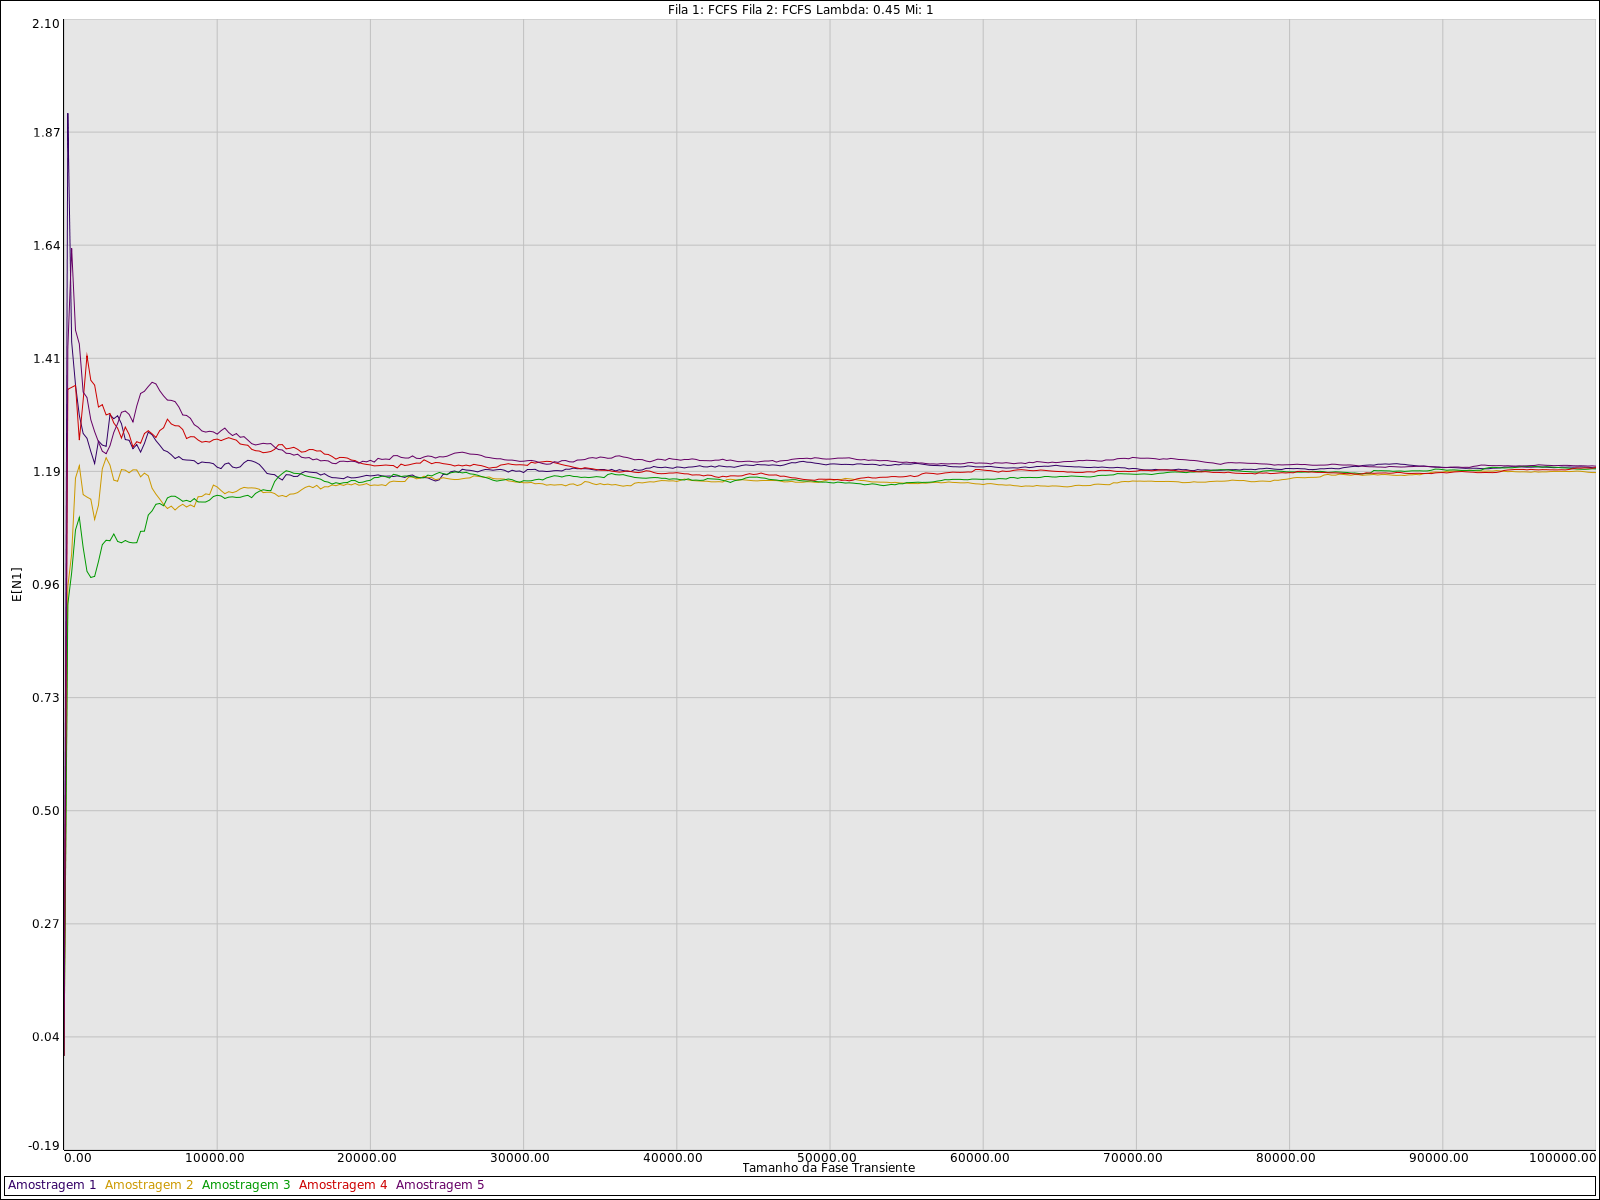
\includegraphics[scale = 0.20]{./graficos_transiente_1/FCFS/01.png}
\end{figure}

\begin{figure}
	\caption{Média da V.A. $N_2$, Serviço FCFS com $\lambda$ = 0.45}
	\label{figTransienteFCFSfila2N}
	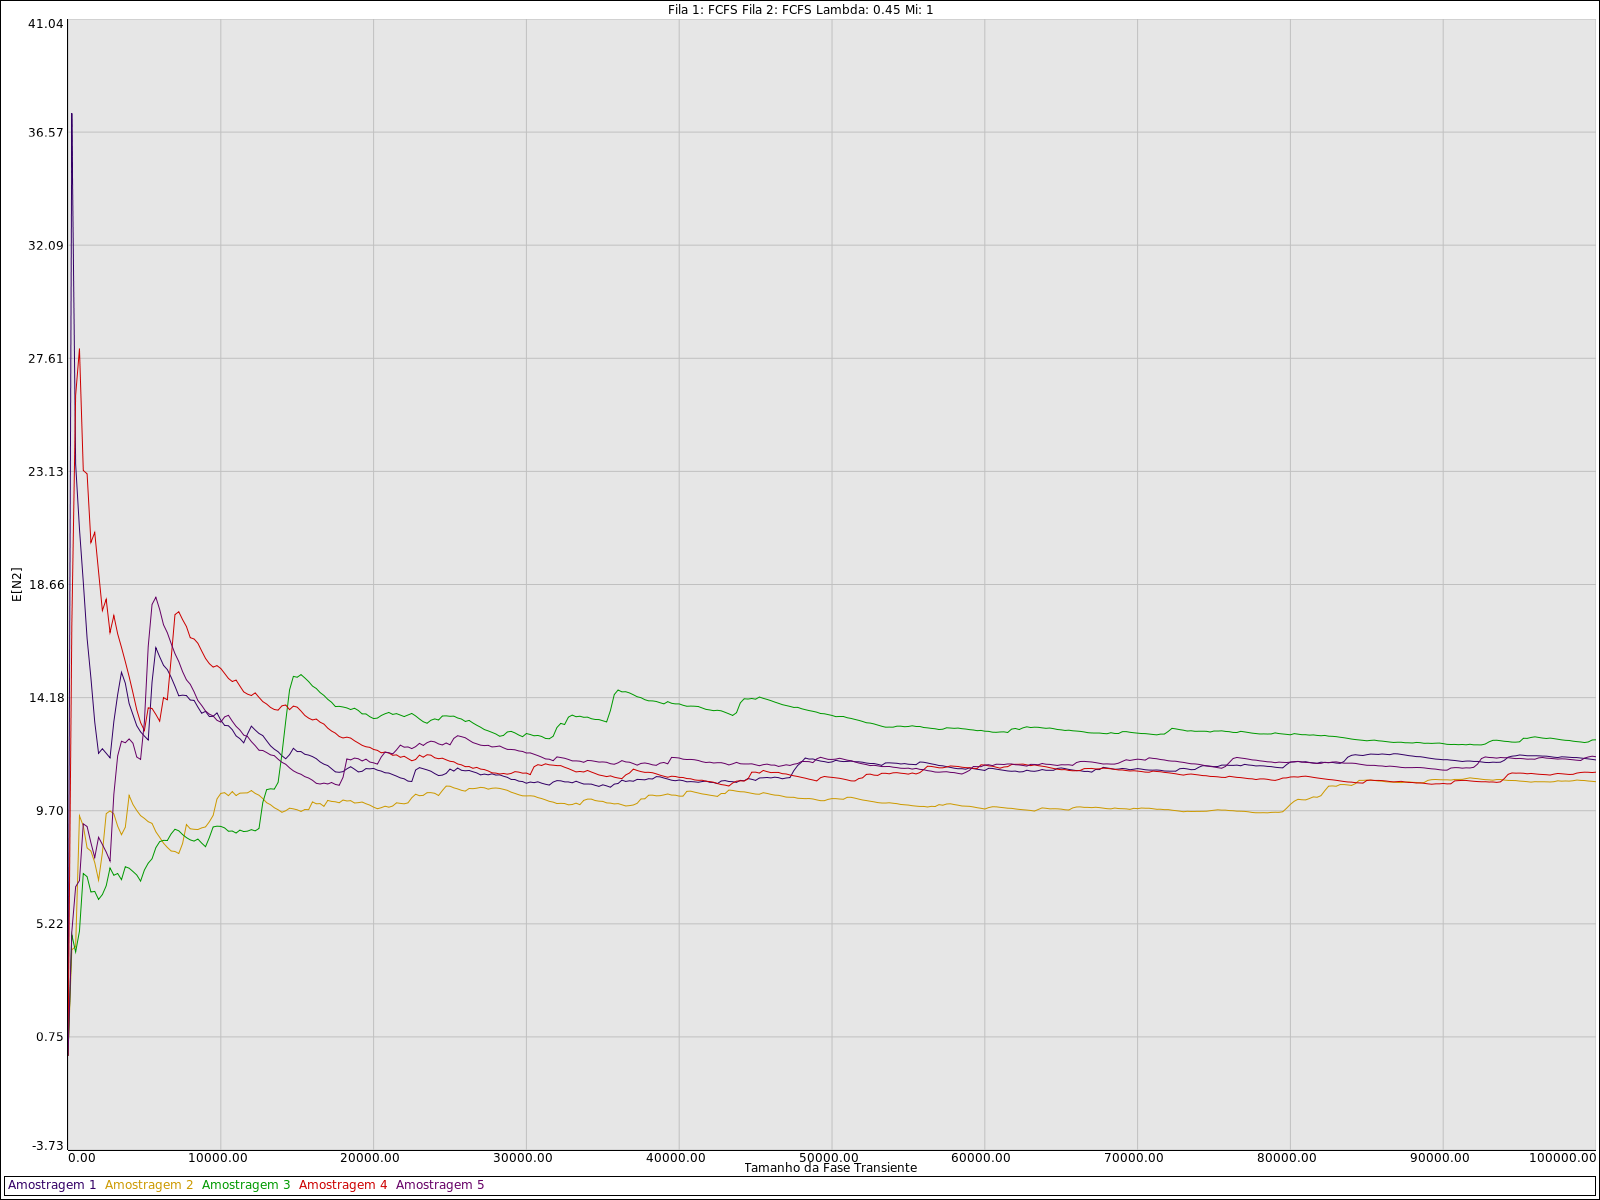
\includegraphics[scale = 0.20]{./graficos_transiente_1/FCFS/02.png}
\end{figure}

\begin{figure}
	\caption{Média da V.A. $Nq_1$, Serviço FCFS com $\lambda$ = 0.45}
	\label{figTransienteFCFSfila1Nq}
	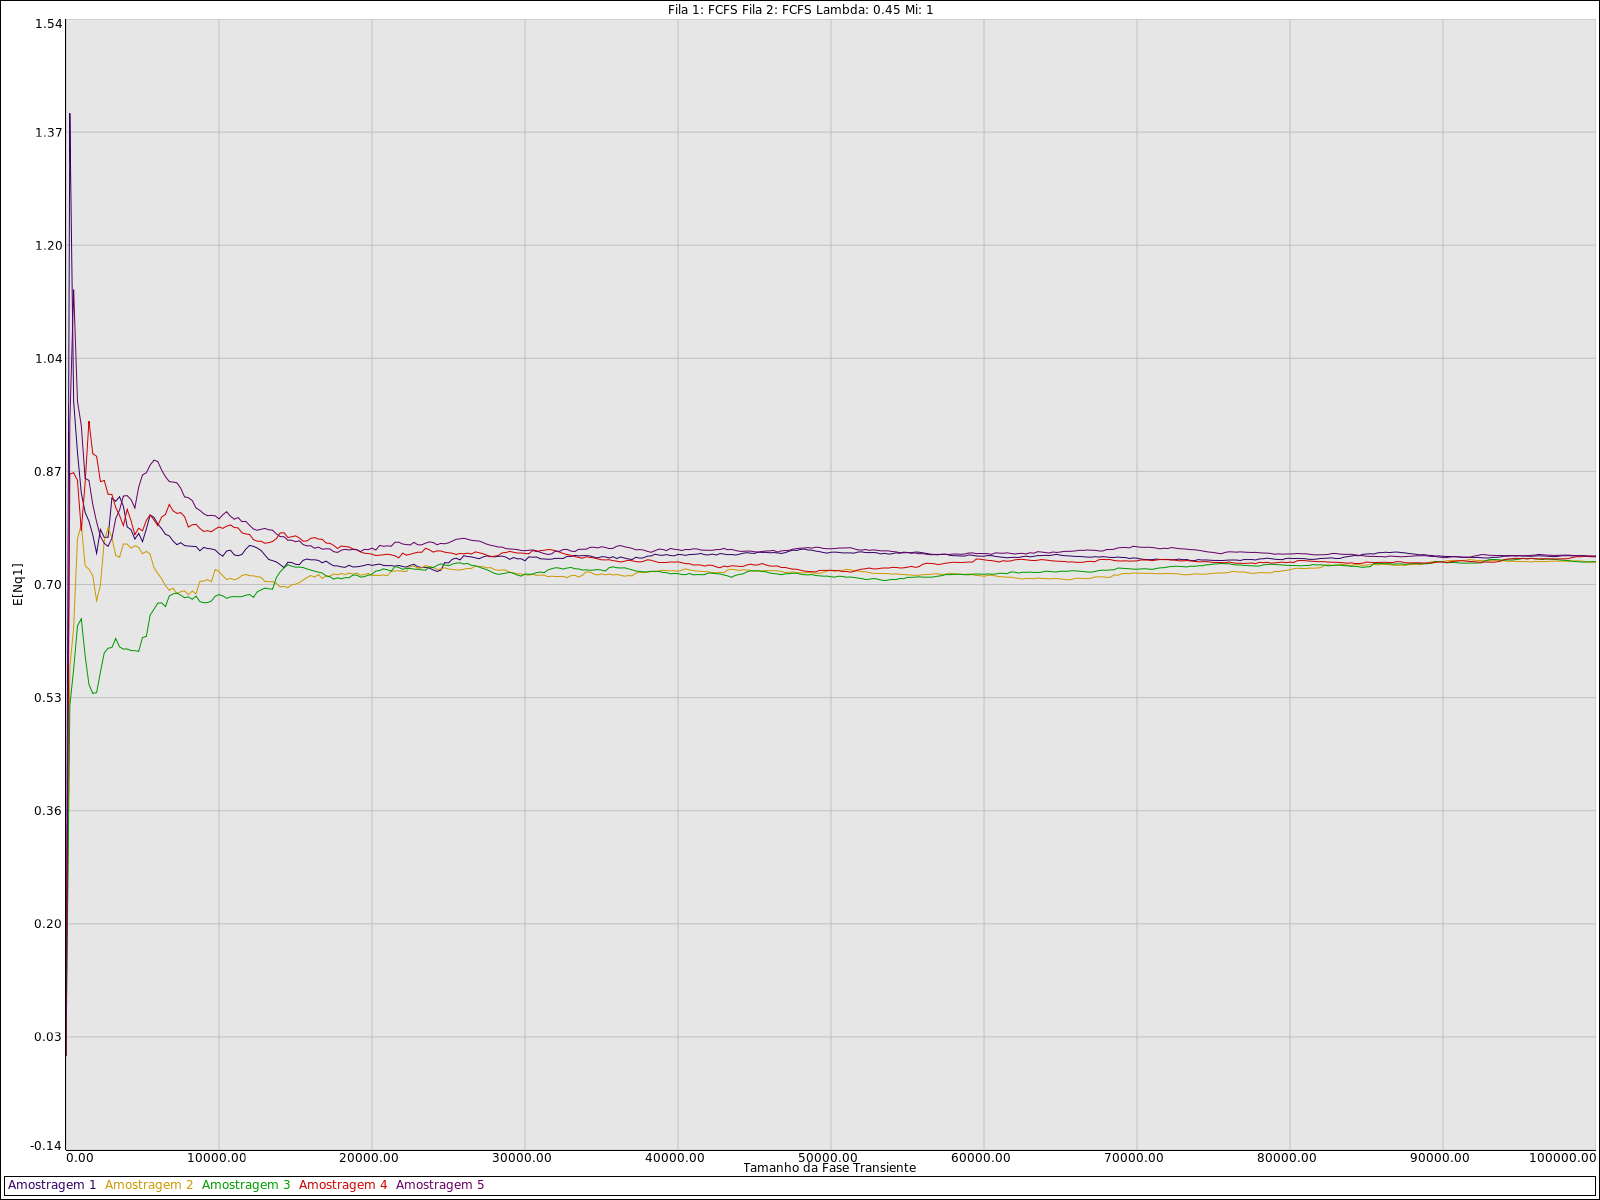
\includegraphics[scale = 0.20]{./graficos_transiente_1/FCFS/03.png}
\end{figure}

\begin{figure}
	\caption{Média da V.A. $Nq_2$, Serviço FCFS com $\lambda$ = 0.45}
	\label{figTransienteFCFSfila2Nq}
	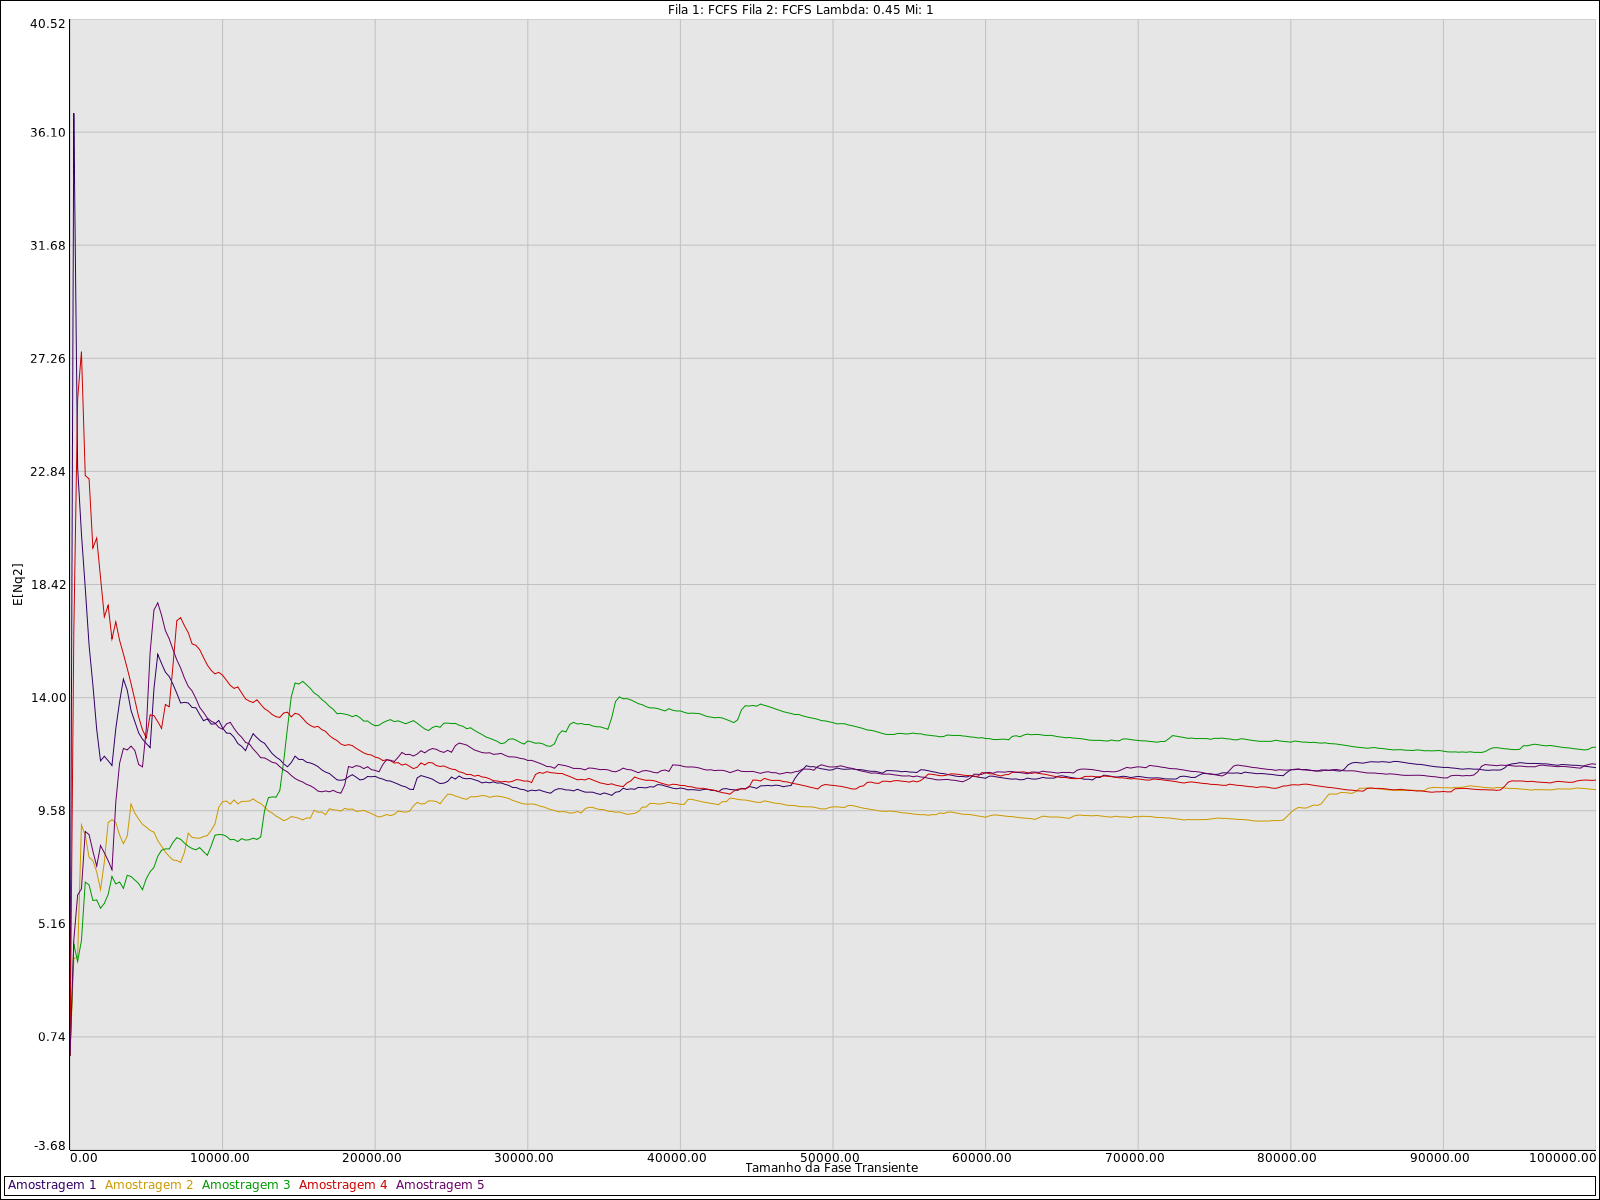
\includegraphics[scale = 0.20]{./graficos_transiente_1/FCFS/04.png}
\end{figure}

\begin{figure}
	\caption{Média da V.A. $T_1$, Serviço FCFS com $\lambda$ = 0.45}
	\label{figTransienteFCFSfila1T}
	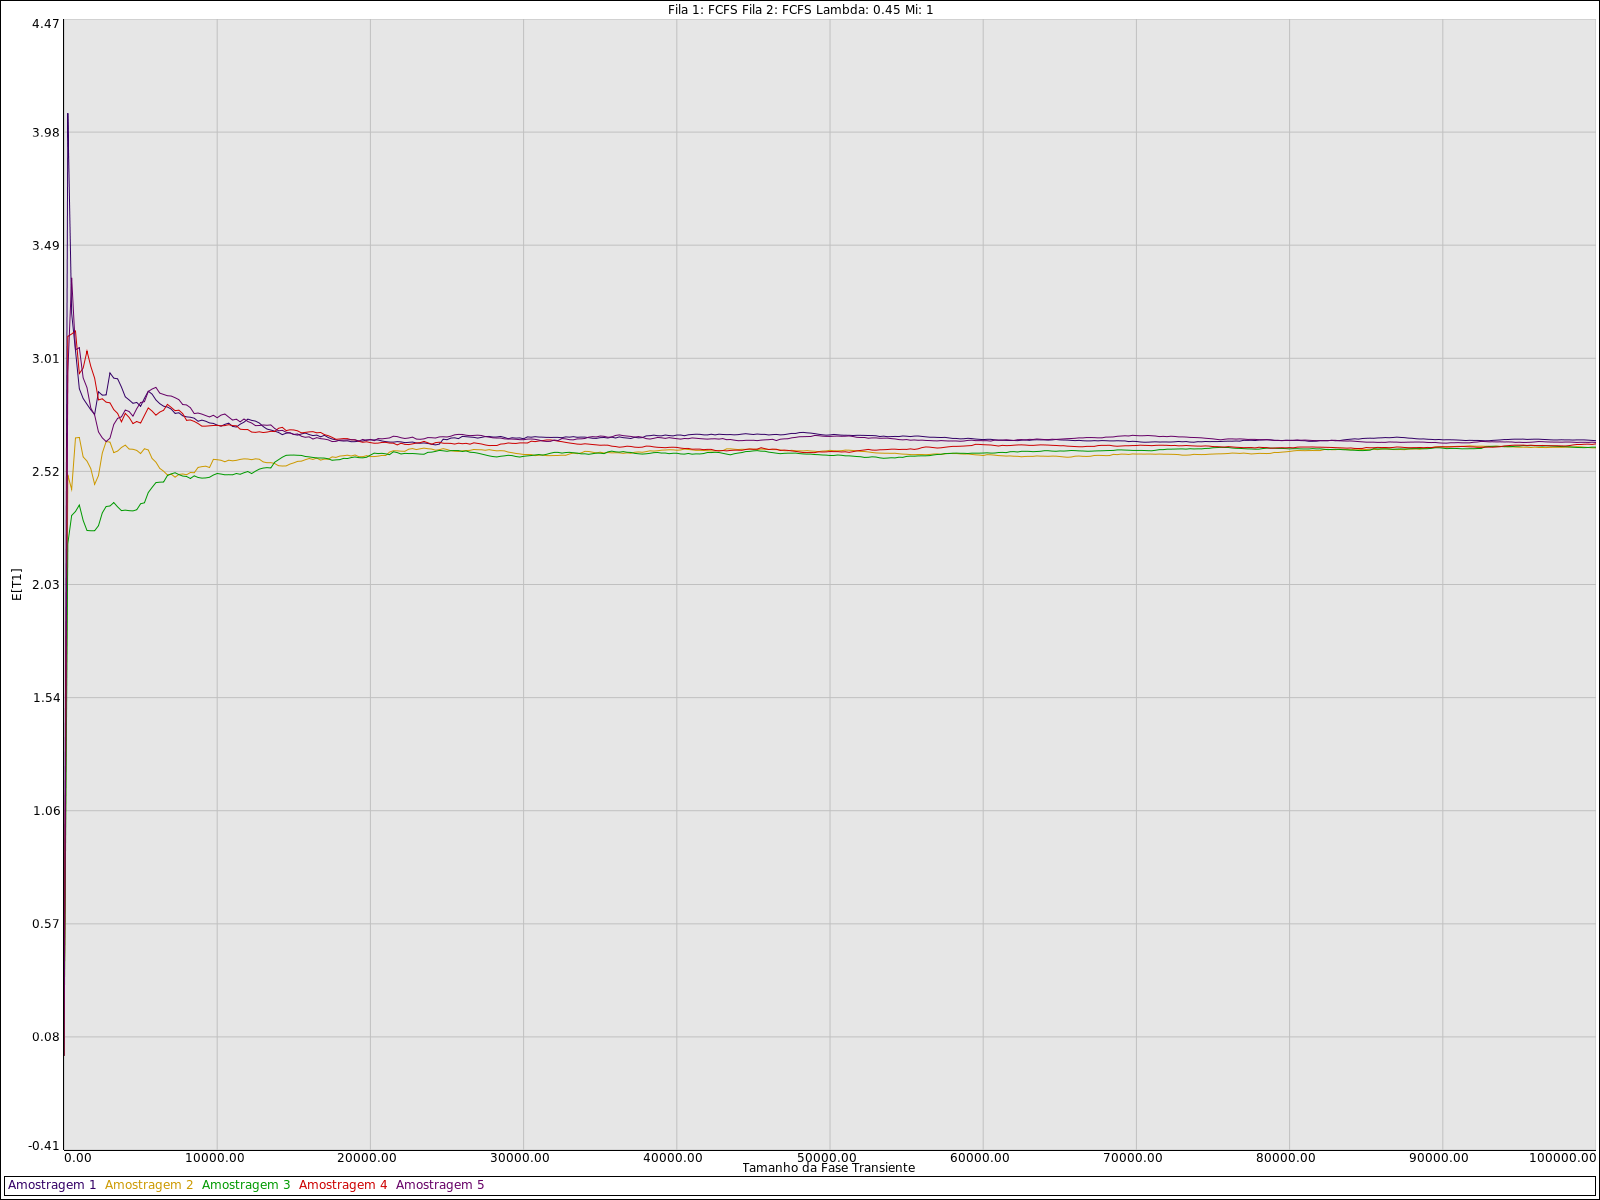
\includegraphics[scale = 0.20]{./graficos_transiente_1/FCFS/05.png}
\end{figure}

\begin{figure}
	\caption{Média da V.A. $T_2$, Serviço FCFS com $\lambda$ = 0.45}
	\label{figTransienteFCFSfila2T}
	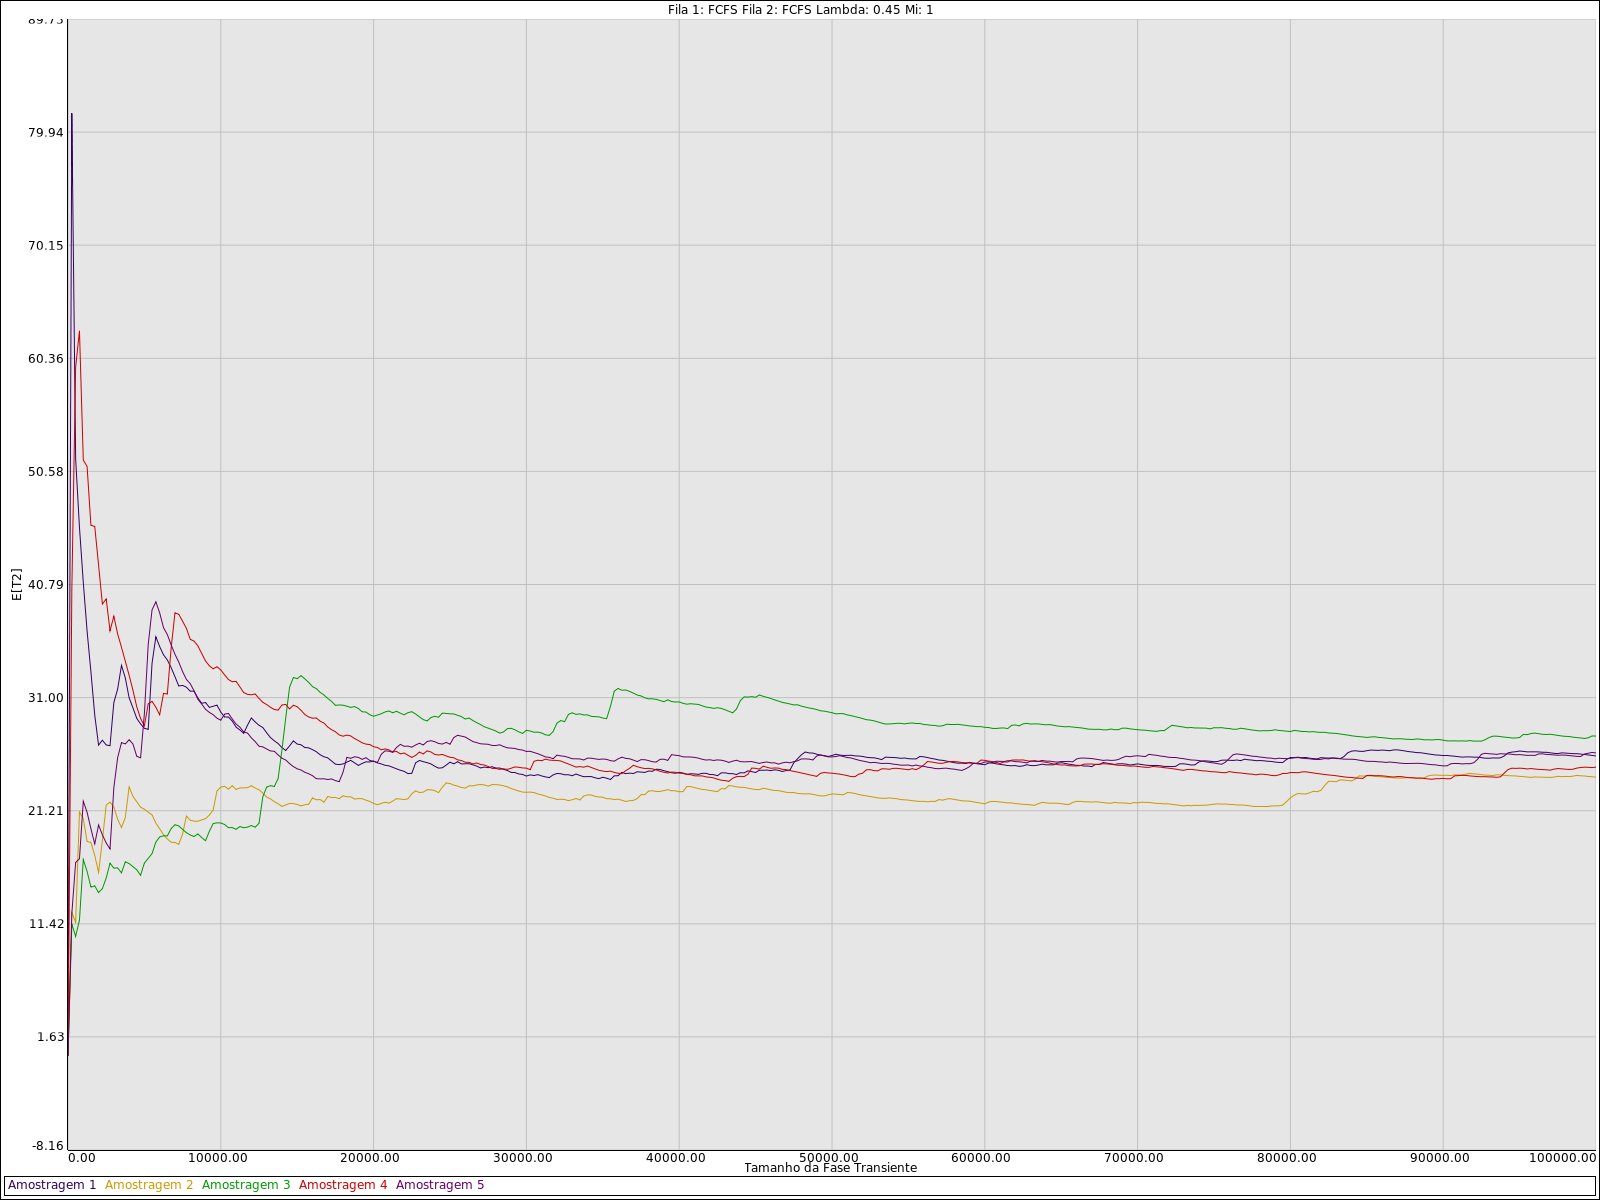
\includegraphics[scale = 0.20]{./graficos_transiente_1/FCFS/06.png}
\end{figure}

\begin{figure}
	\caption{Média da V.A. $W_1$, Serviço FCFS com $\lambda$ = 0.45}
	\label{figTransienteFCFSfila1W}
	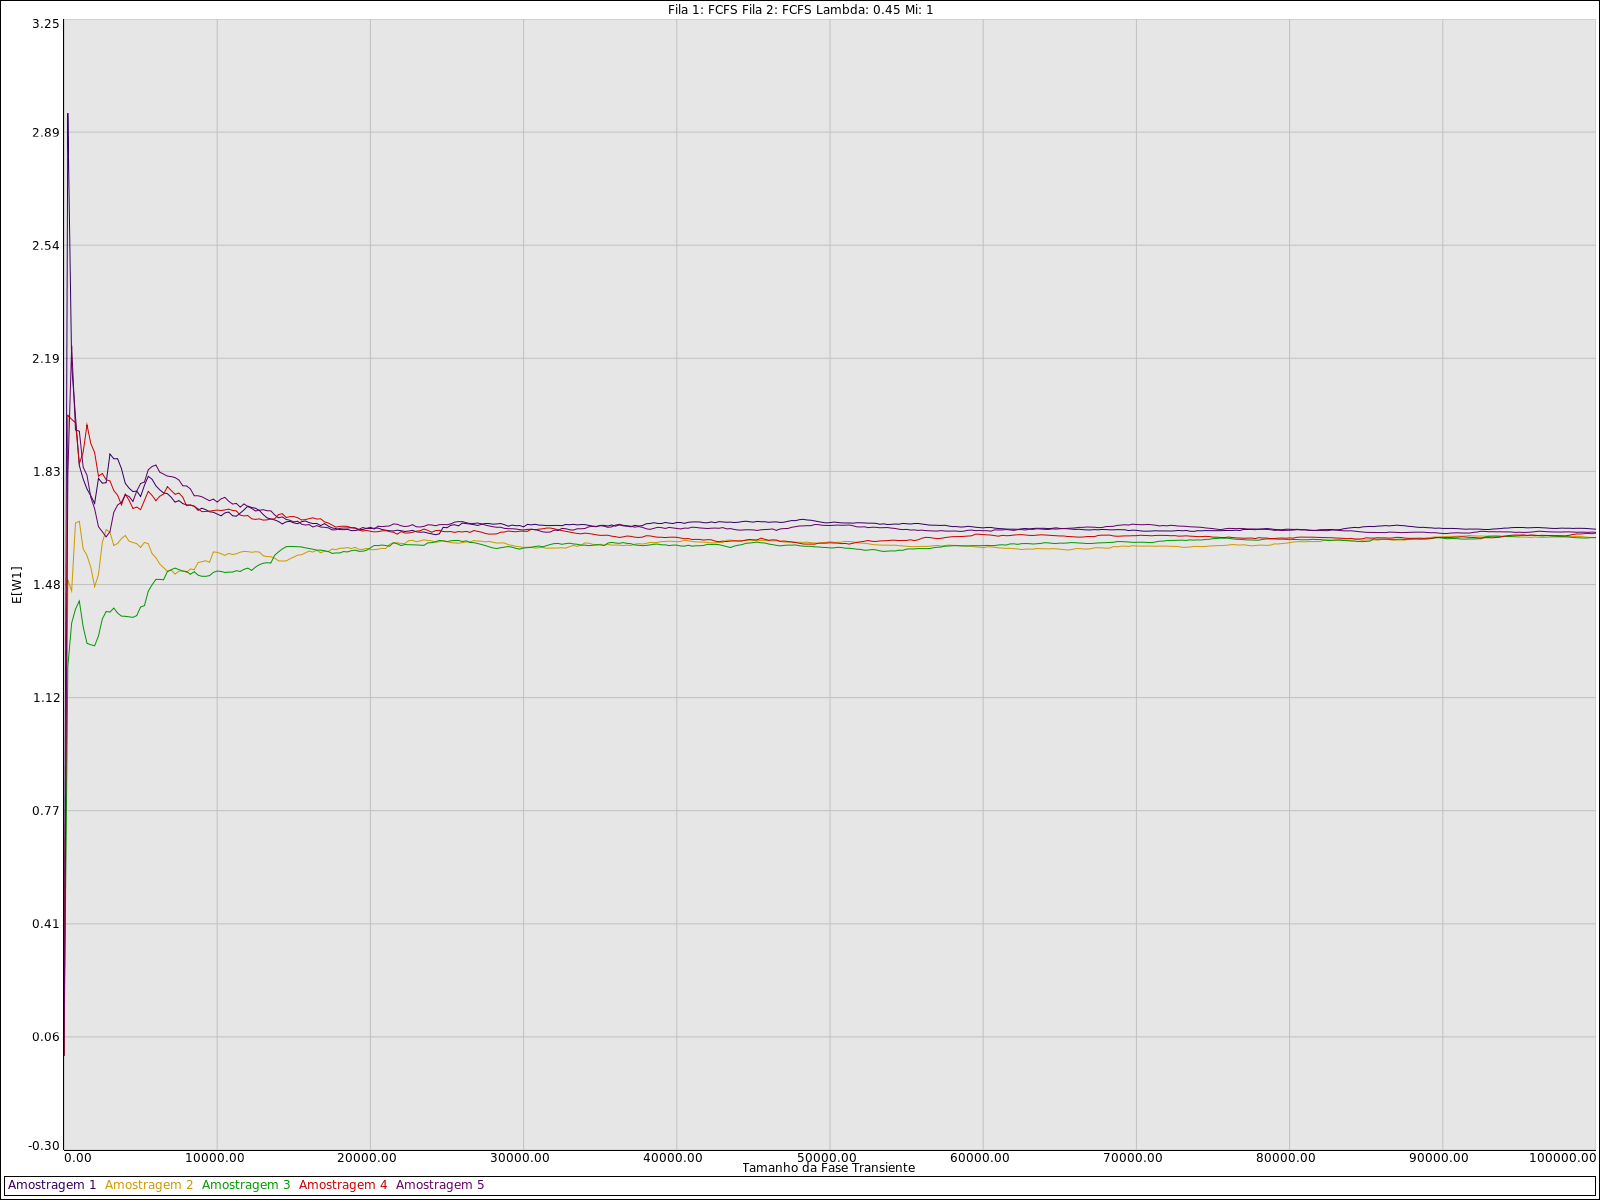
\includegraphics[scale = 0.20]{./graficos_transiente_1/FCFS/07.png}
\end{figure}

\begin{figure}
	\caption{Média da V.A. $W_2$, Serviço FCFS com $\lambda$ = 0.45}
	\label{figTransienteFCFSfila2W}
	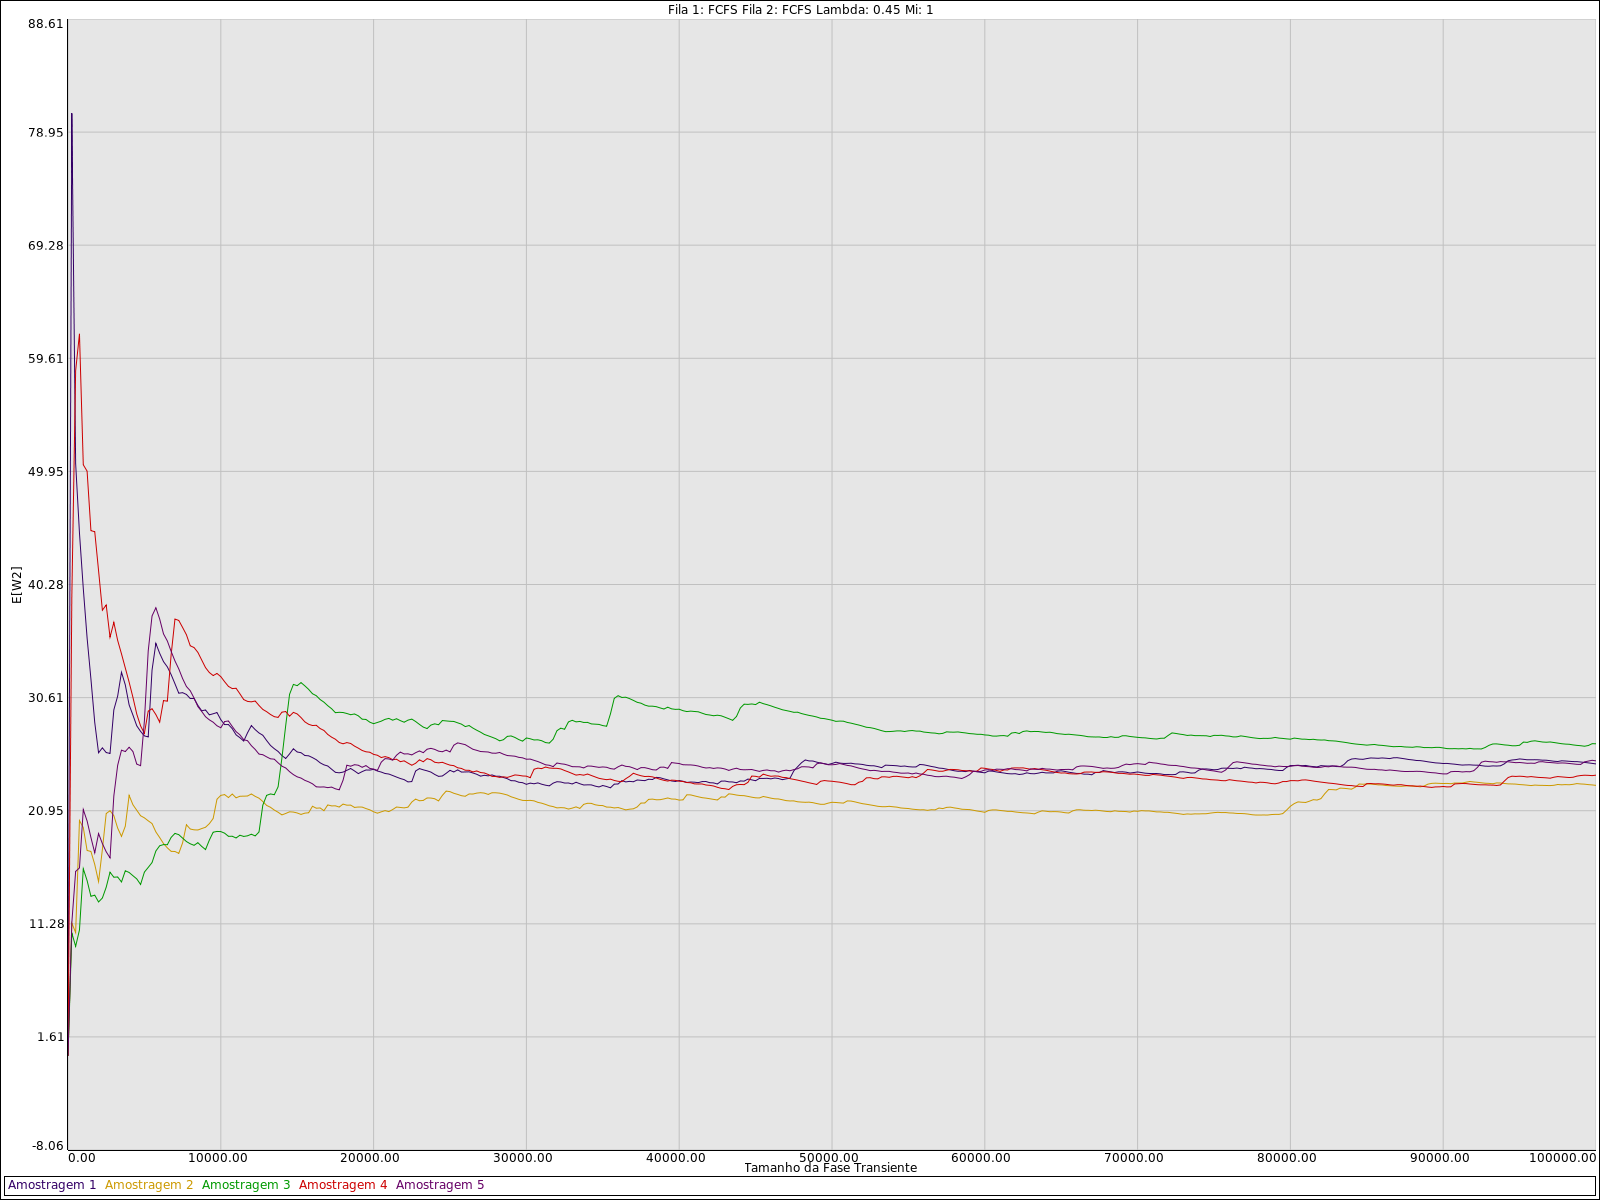
\includegraphics[scale = 0.20]{./graficos_transiente_1/FCFS/08.png}
\end{figure}

\begin{figure}
	\caption{Variância da V.A. $W_1$, Serviço FCFS com $\lambda$ = 0.45}
	\label{figTransienteFCFSfila1VarW}
	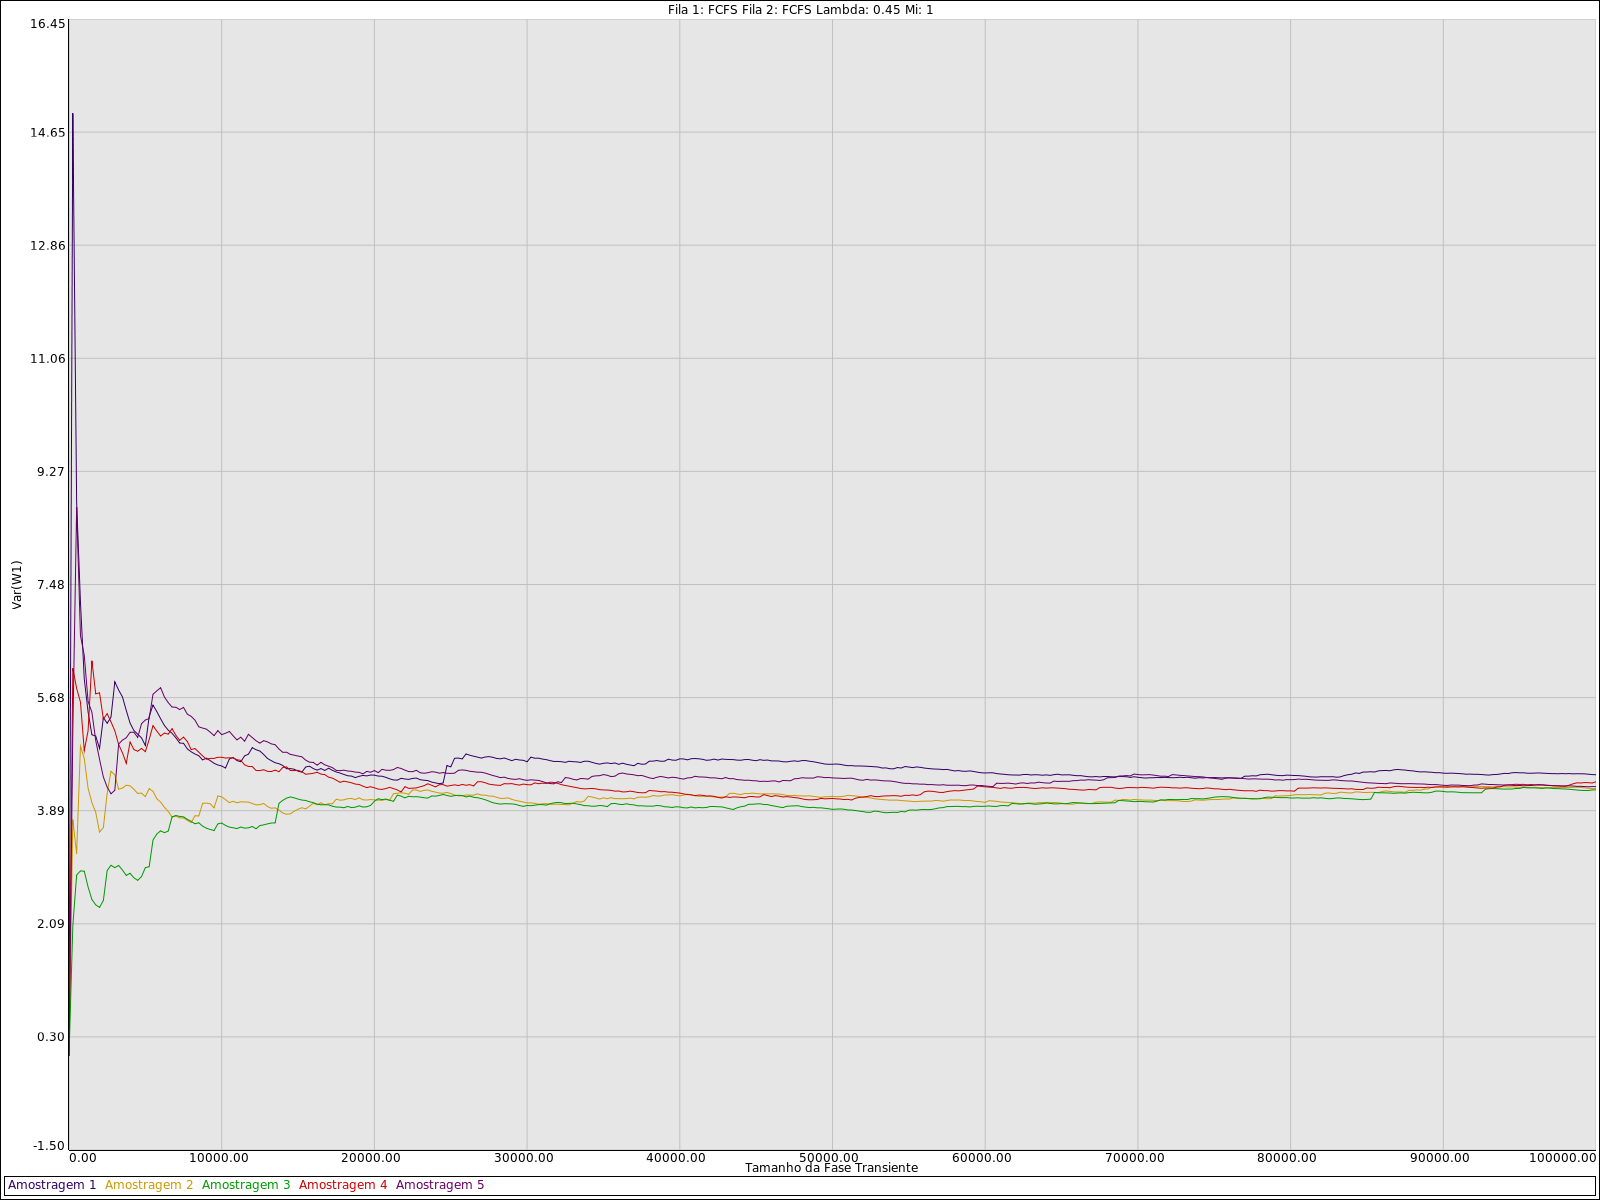
\includegraphics[scale = 0.20]{./graficos_transiente_1/FCFS/09.png}
\end{figure}

\begin{figure}
	\caption{Variância da V.A. $W_2$, Serviço FCFS com $\lambda$ = 0.45}
	\label{figTransienteFCFSfila2VarW}
	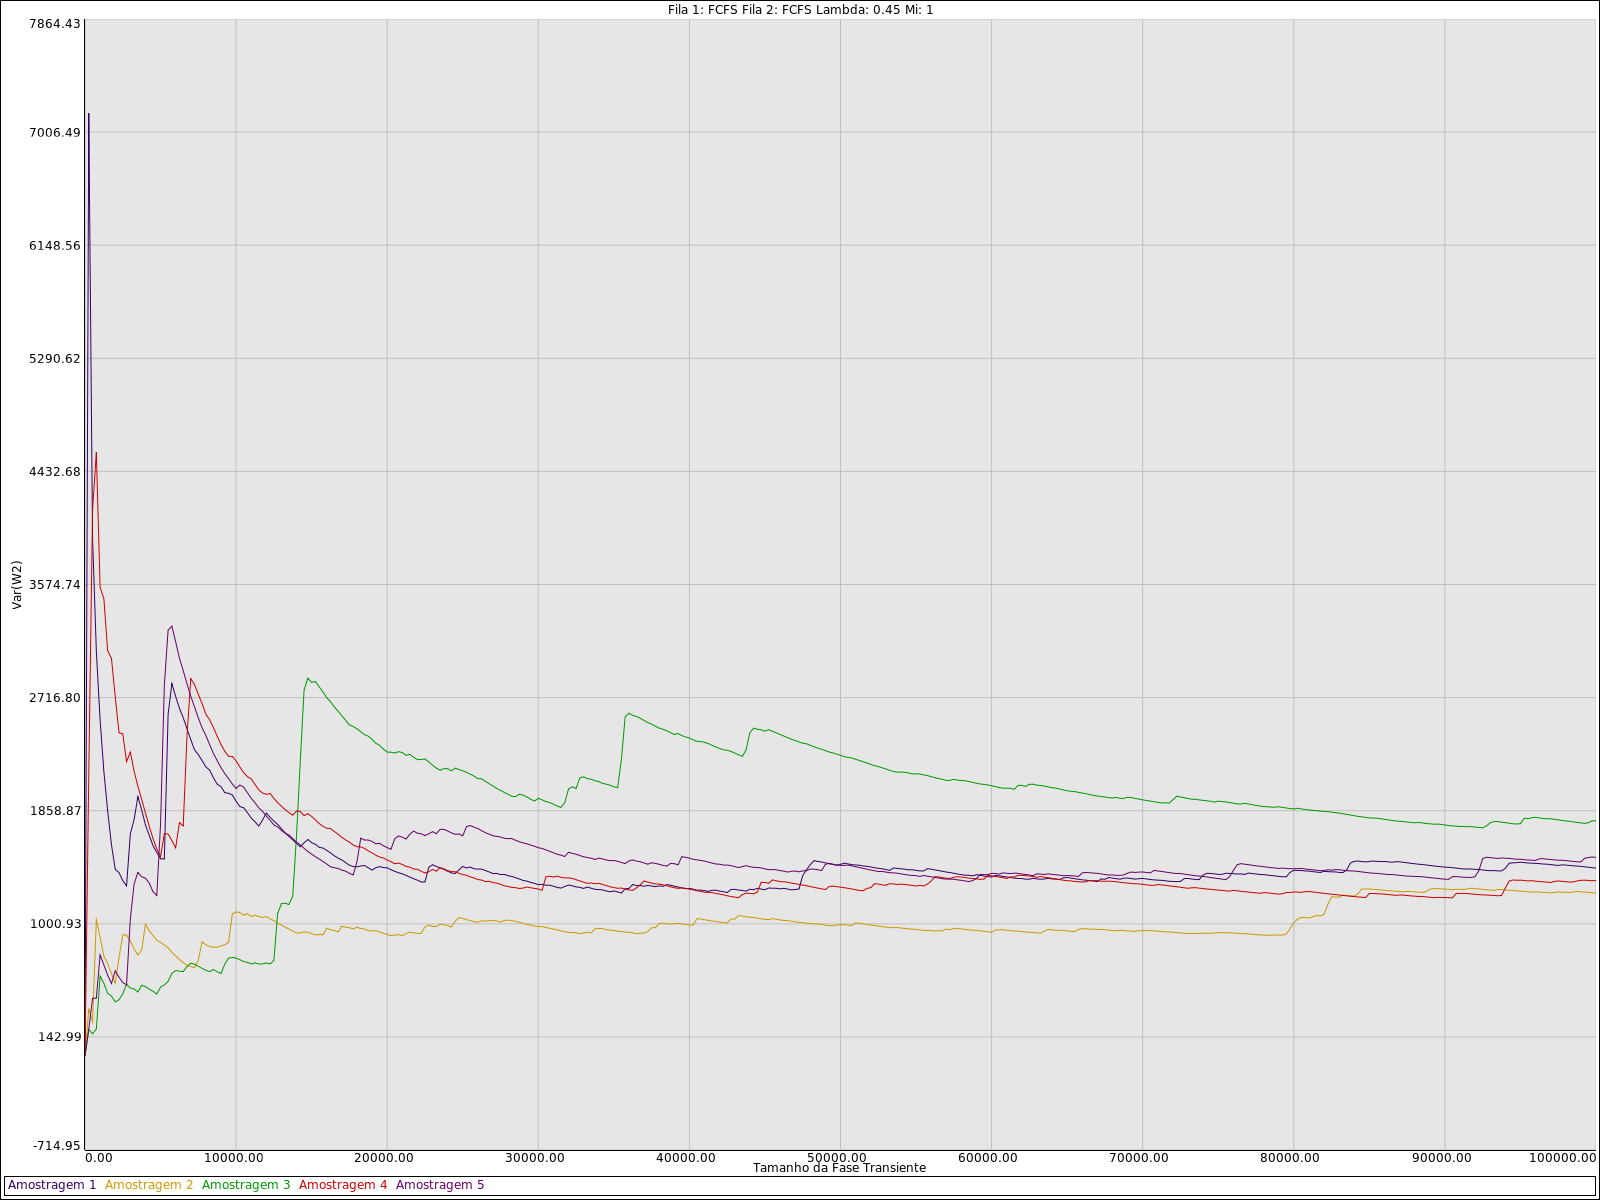
\includegraphics[scale = 0.20]{./graficos_transiente_1/FCFS/10.png}
\end{figure}

\clearpage

%figuras do LCFS pra 50k de transiente
\begin{figure}
	\caption{Média da V.A. $N_1$, Serviço LCFS com $\lambda$ = 0.45}
	\label{figTransienteLCFSfila1N}
	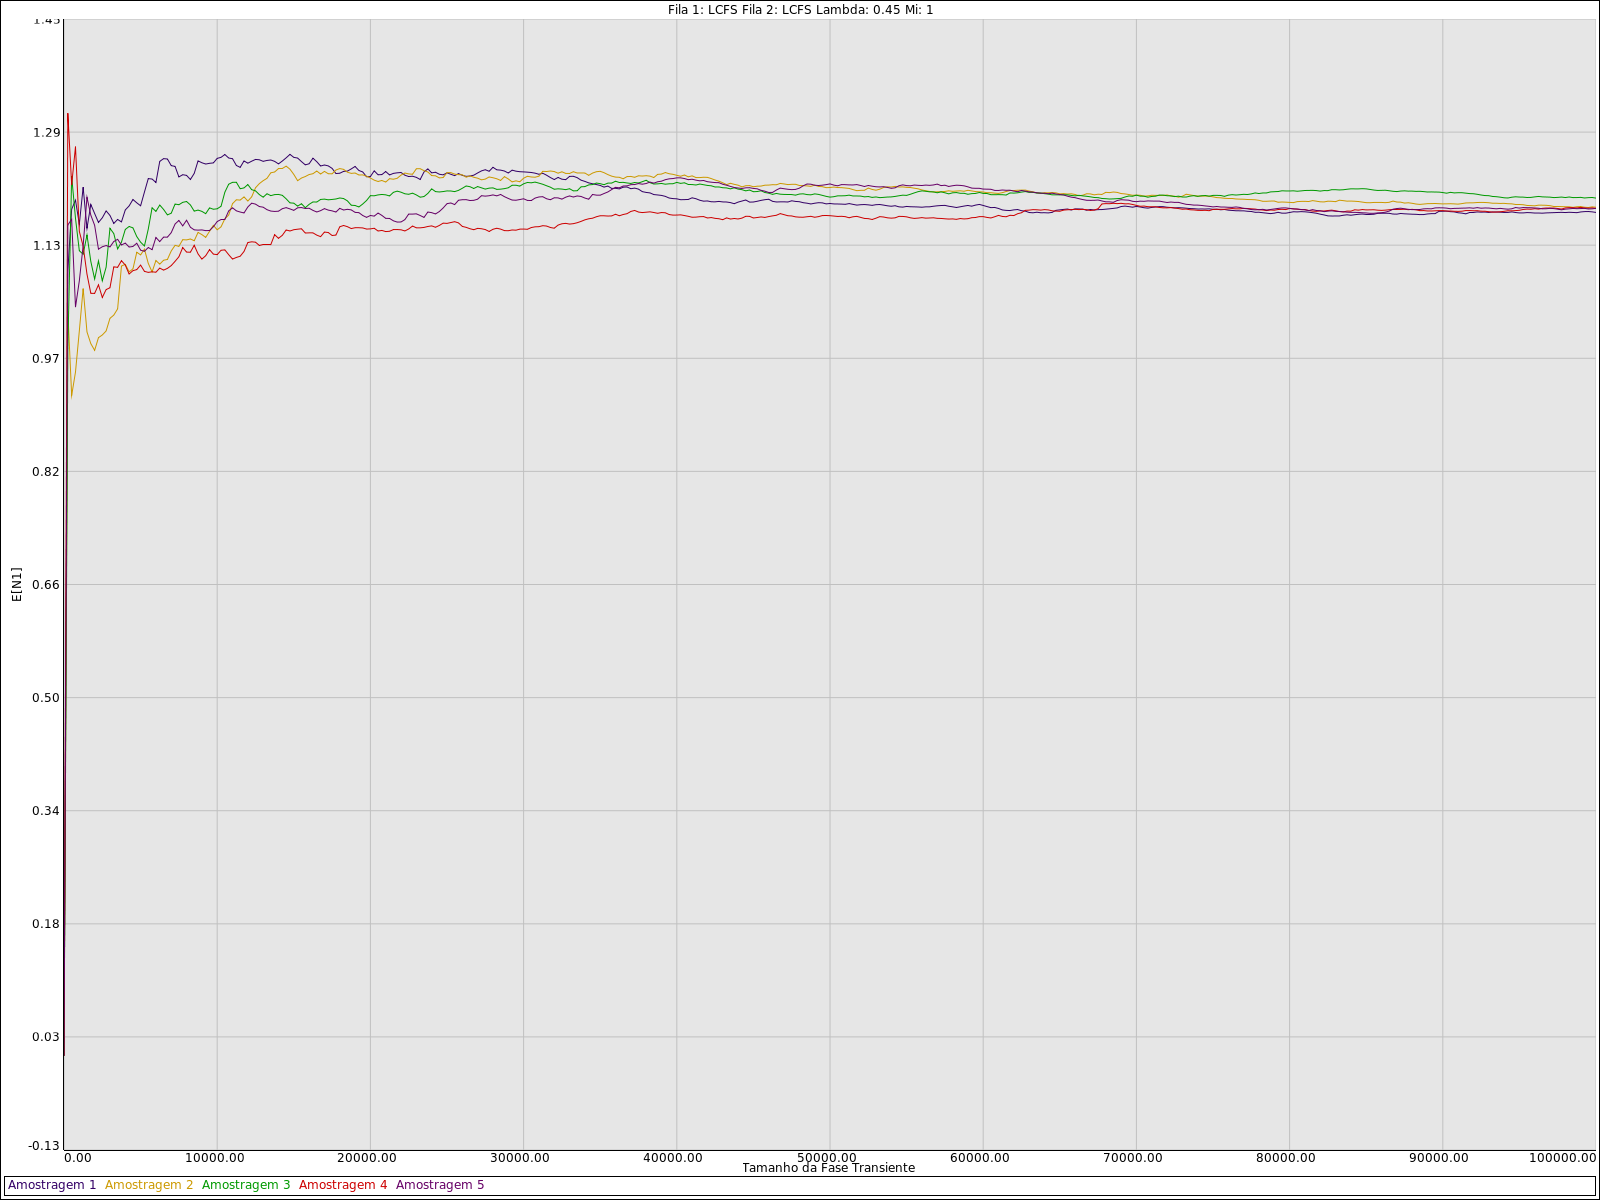
\includegraphics[scale = 0.20]{./graficos_transiente_1/LCFS/01.png}
\end{figure}

\begin{figure}
	\caption{Média da V.A. $N_2$, Serviço LCFS com $\lambda$ = 0.45}
	\label{figTransienteLCFSfila2N}
	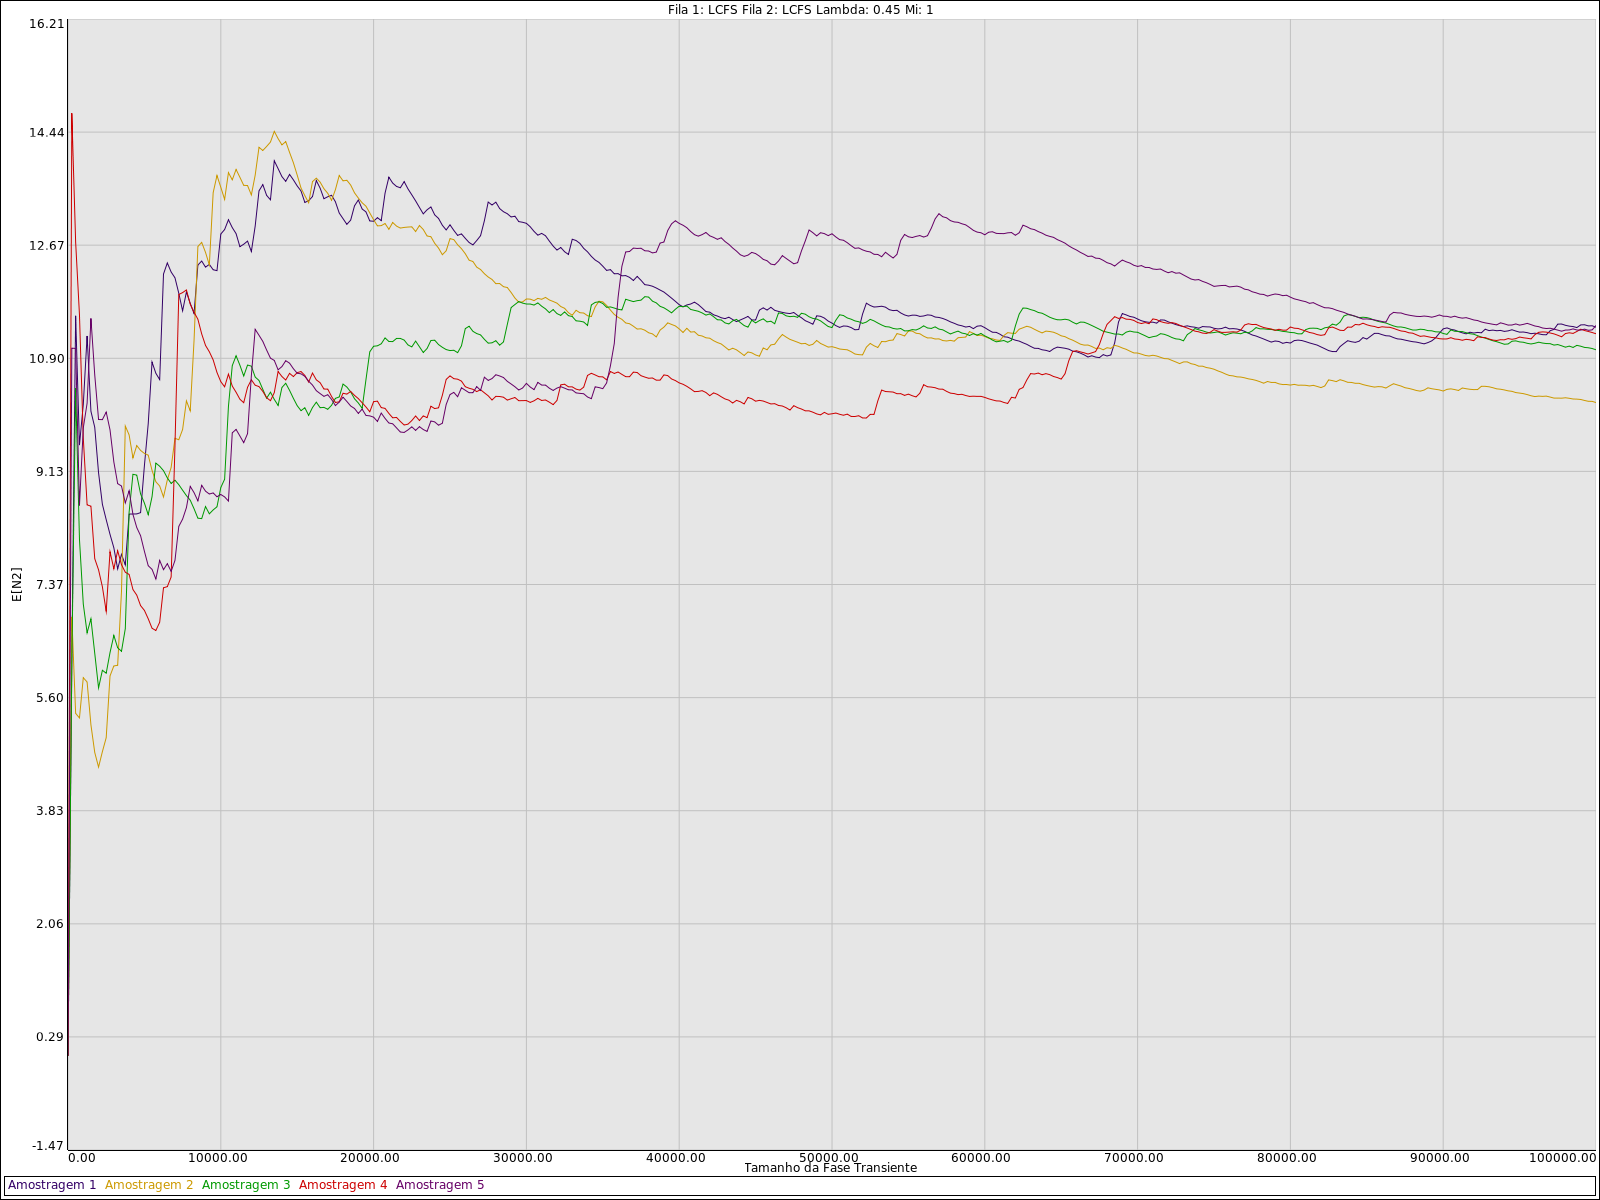
\includegraphics[scale = 0.20]{./graficos_transiente_1/LCFS/02.png}
\end{figure}

\begin{figure}
	\caption{Média da V.A. $Nq_1$, Serviço LCFS com $\lambda$ = 0.45}
	\label{figTransienteLCFSfila1Nq}
	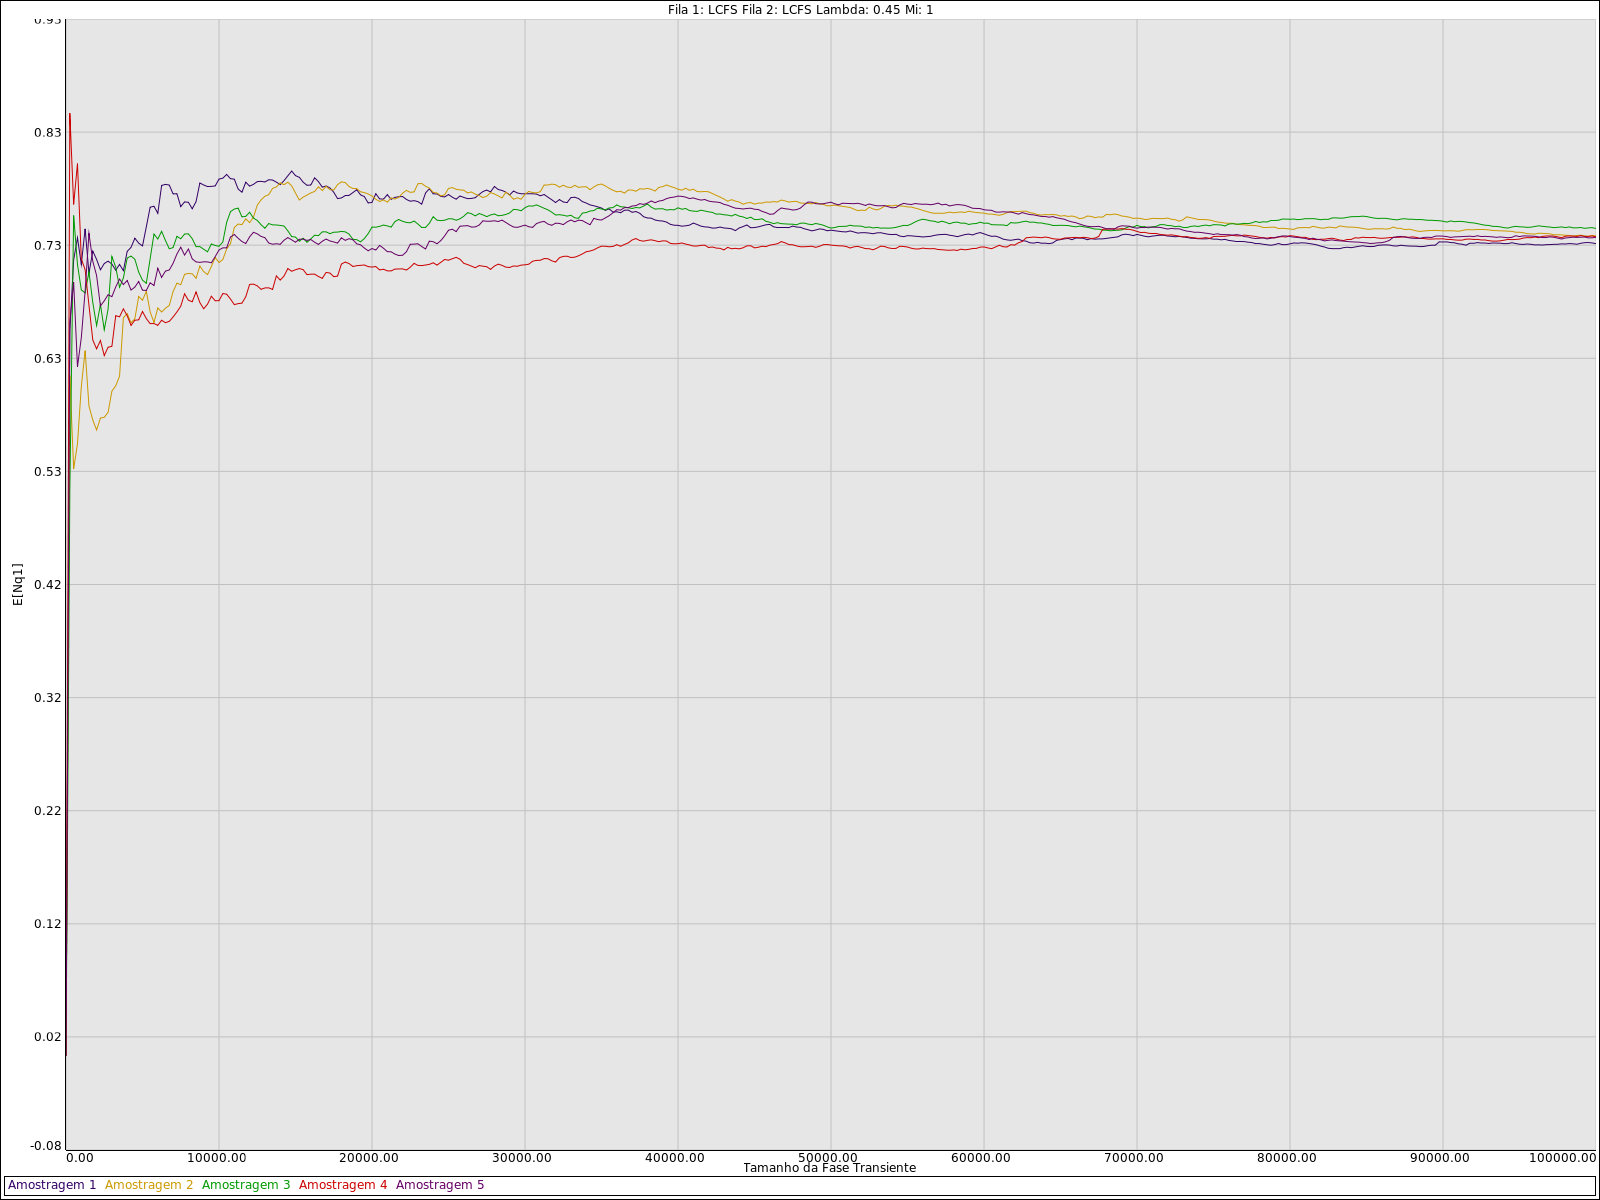
\includegraphics[scale = 0.20]{./graficos_transiente_1/LCFS/03.png}
\end{figure}

\begin{figure}
	\caption{Média da V.A. $Nq_2$, Serviço LCFS com $\lambda$ = 0.45}
	\label{figTransienteLCFSfila2Nq}
	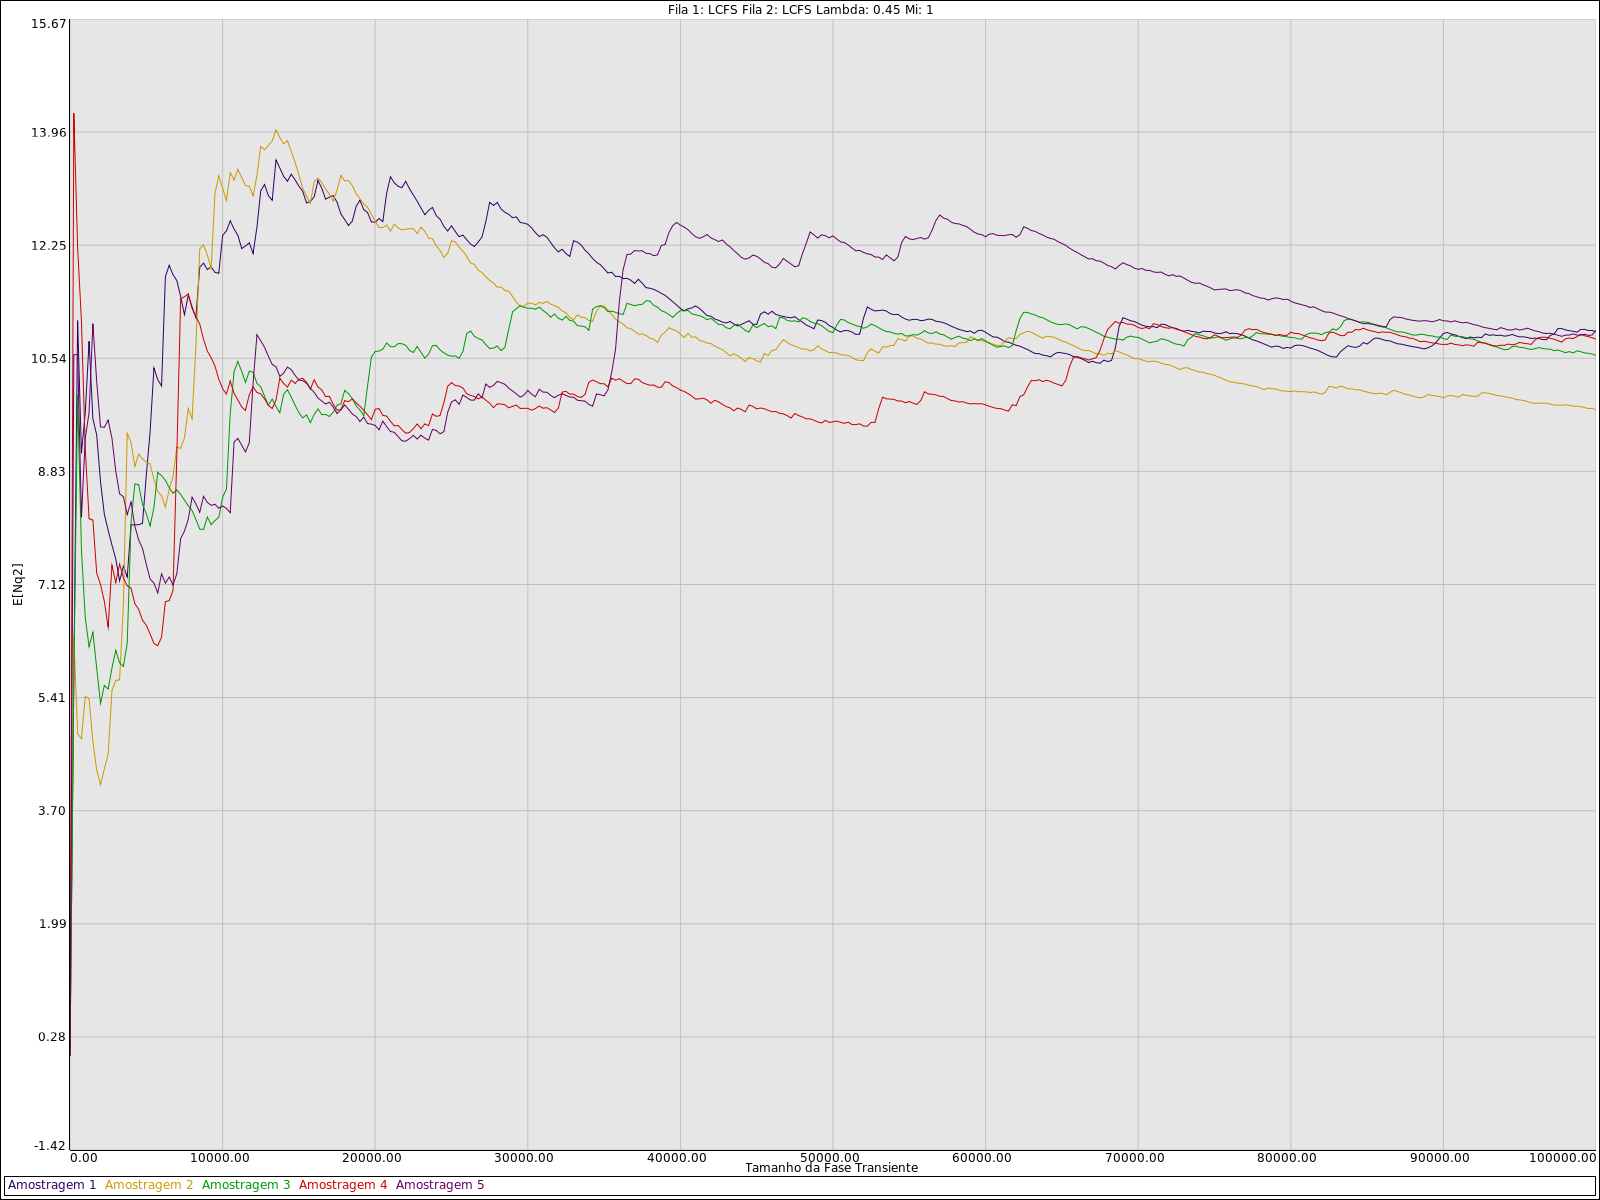
\includegraphics[scale = 0.20]{./graficos_transiente_1/LCFS/04.png}
\end{figure}

\begin{figure}
	\caption{Média da V.A. $T_1$, Serviço LCFS com $\lambda$ = 0.45}
	\label{figTransienteLCFSfila1T}
	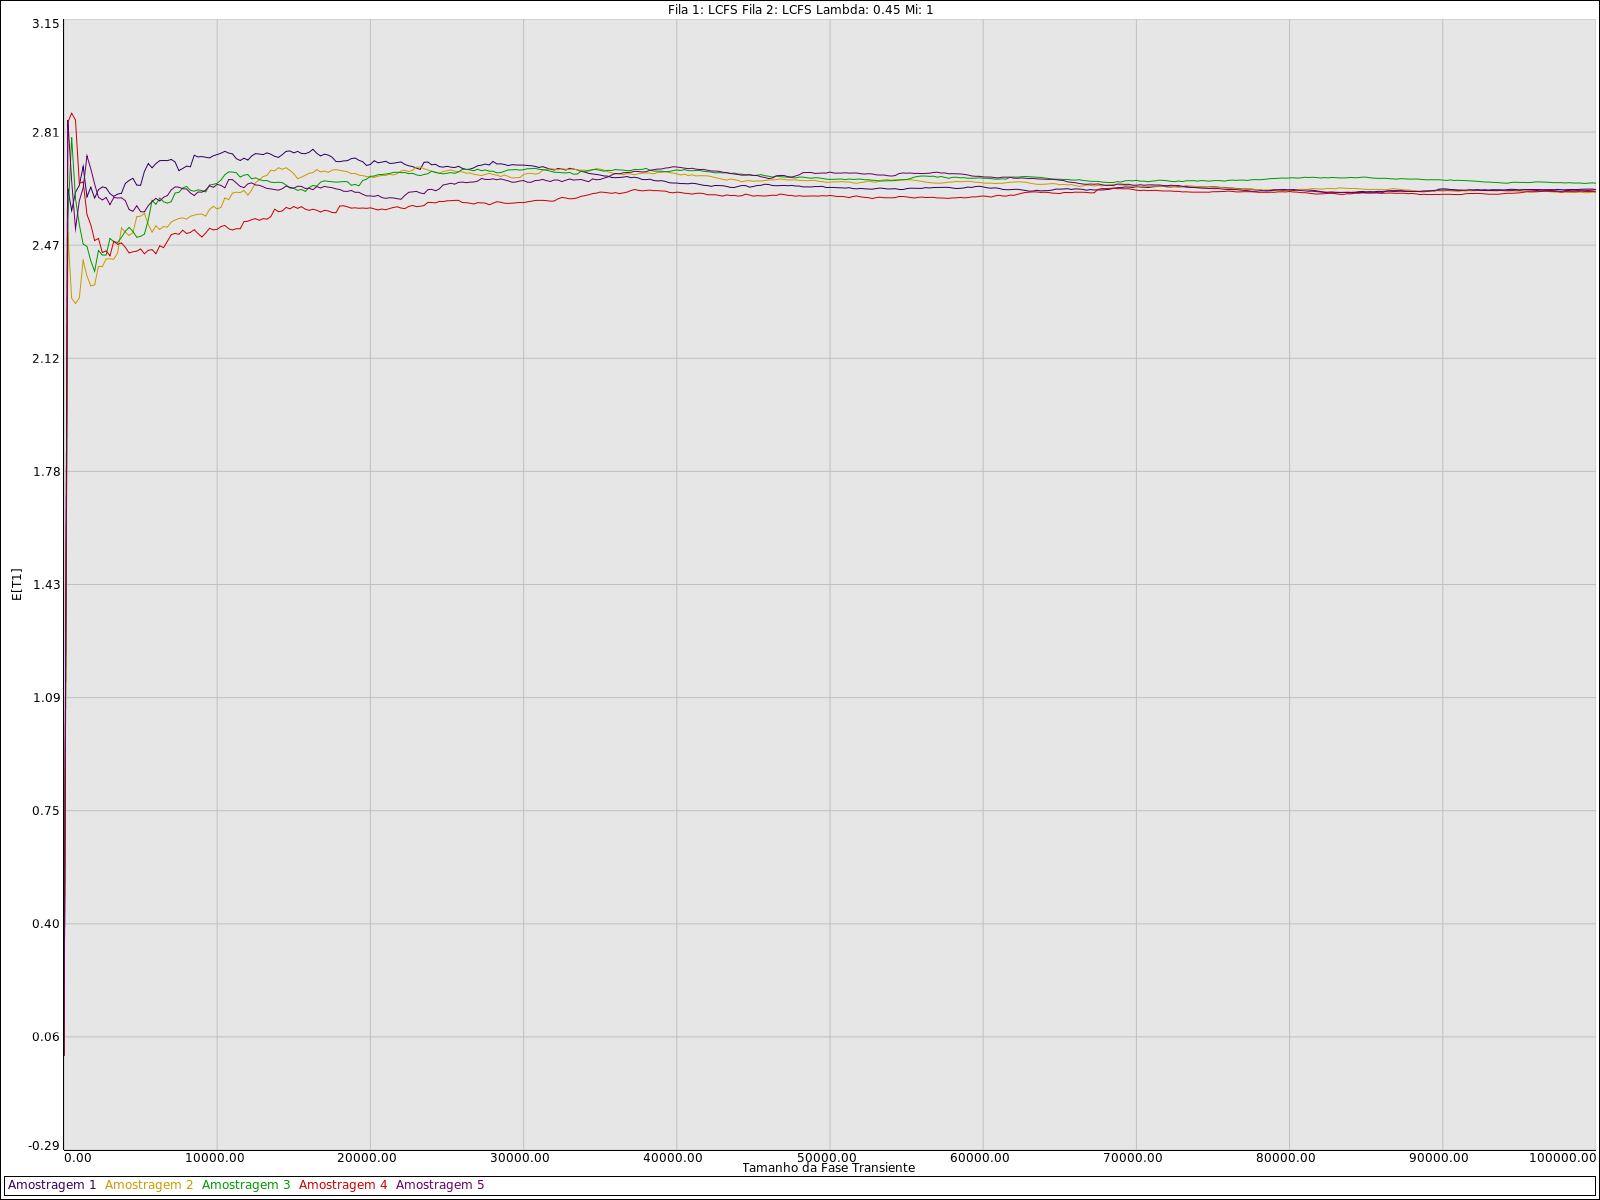
\includegraphics[scale = 0.20]{./graficos_transiente_1/LCFS/05.png}
\end{figure}

\begin{figure}
	\caption{Média da V.A. $T_2$, Serviço LCFS com $\lambda$ = 0.45}
	\label{figTransienteLCFSfila2T}
	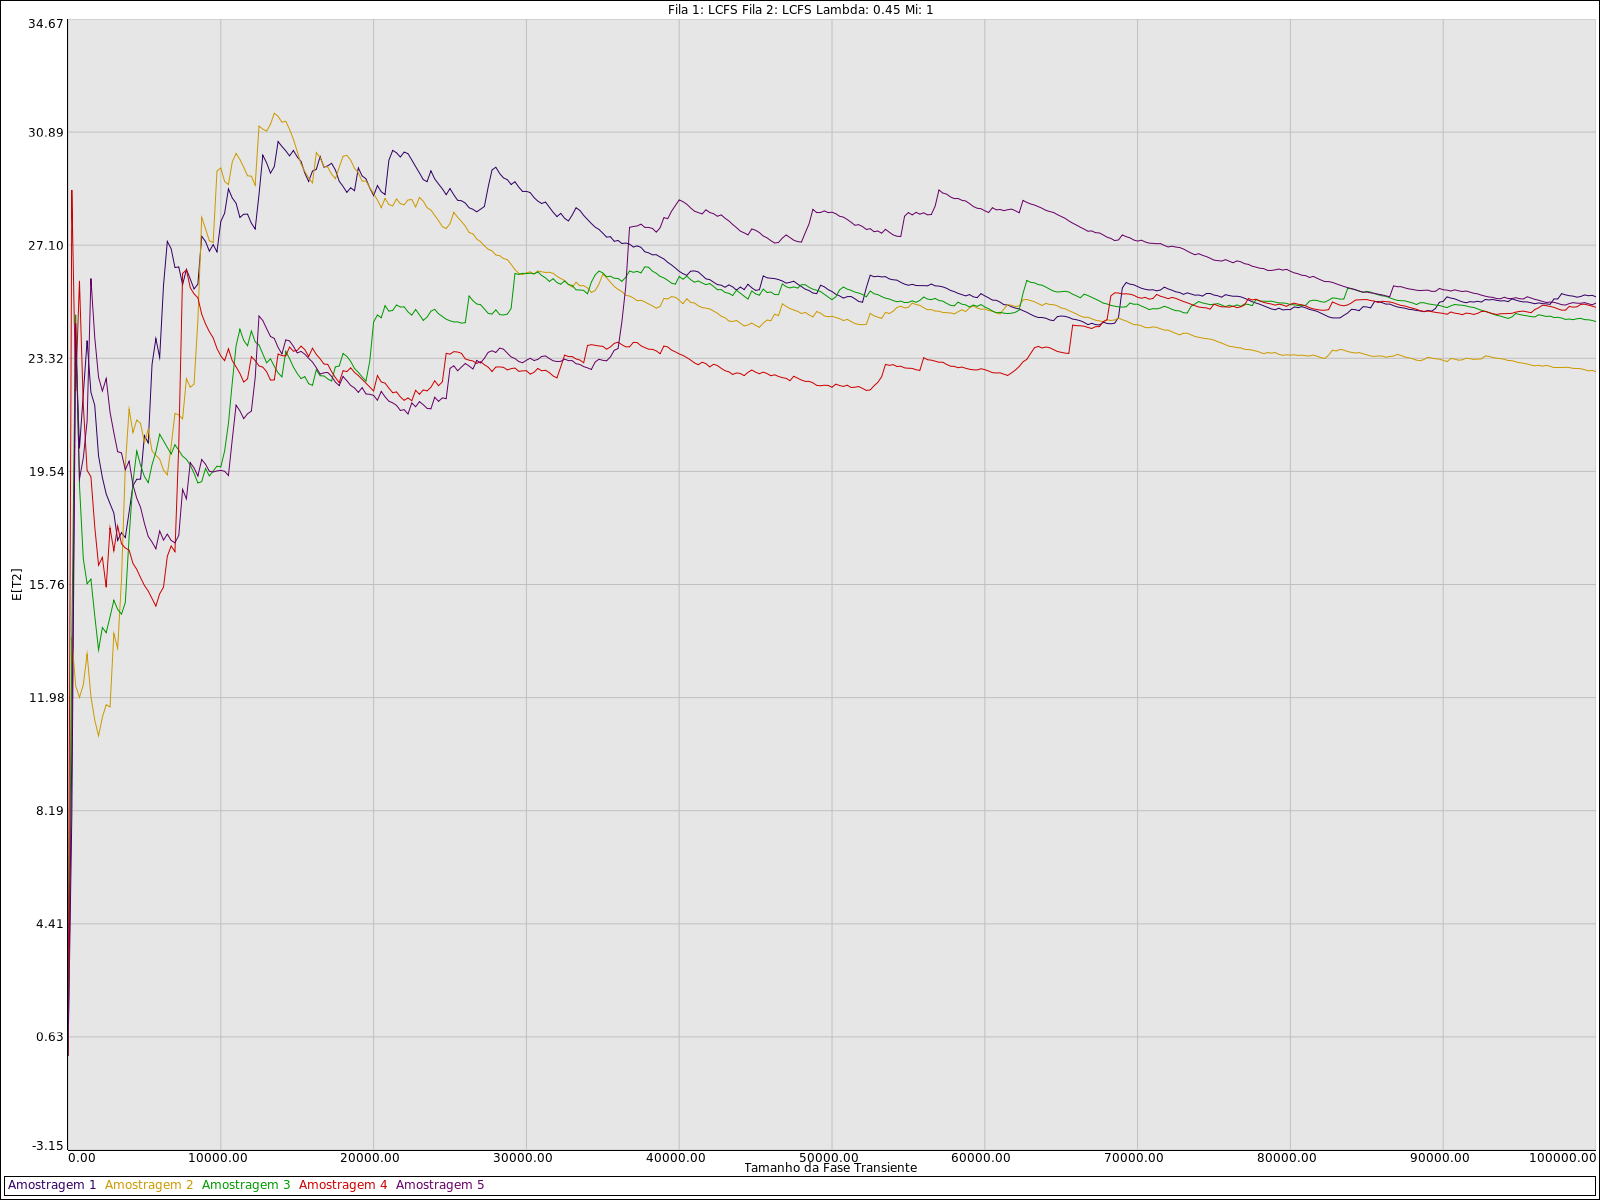
\includegraphics[scale = 0.20]{./graficos_transiente_1/LCFS/06.png}
\end{figure}

\begin{figure}
	\caption{Média da V.A. $W_1$, Serviço LCFS com $\lambda$ = 0.45}
	\label{figTransienteLCFSfila1W}
	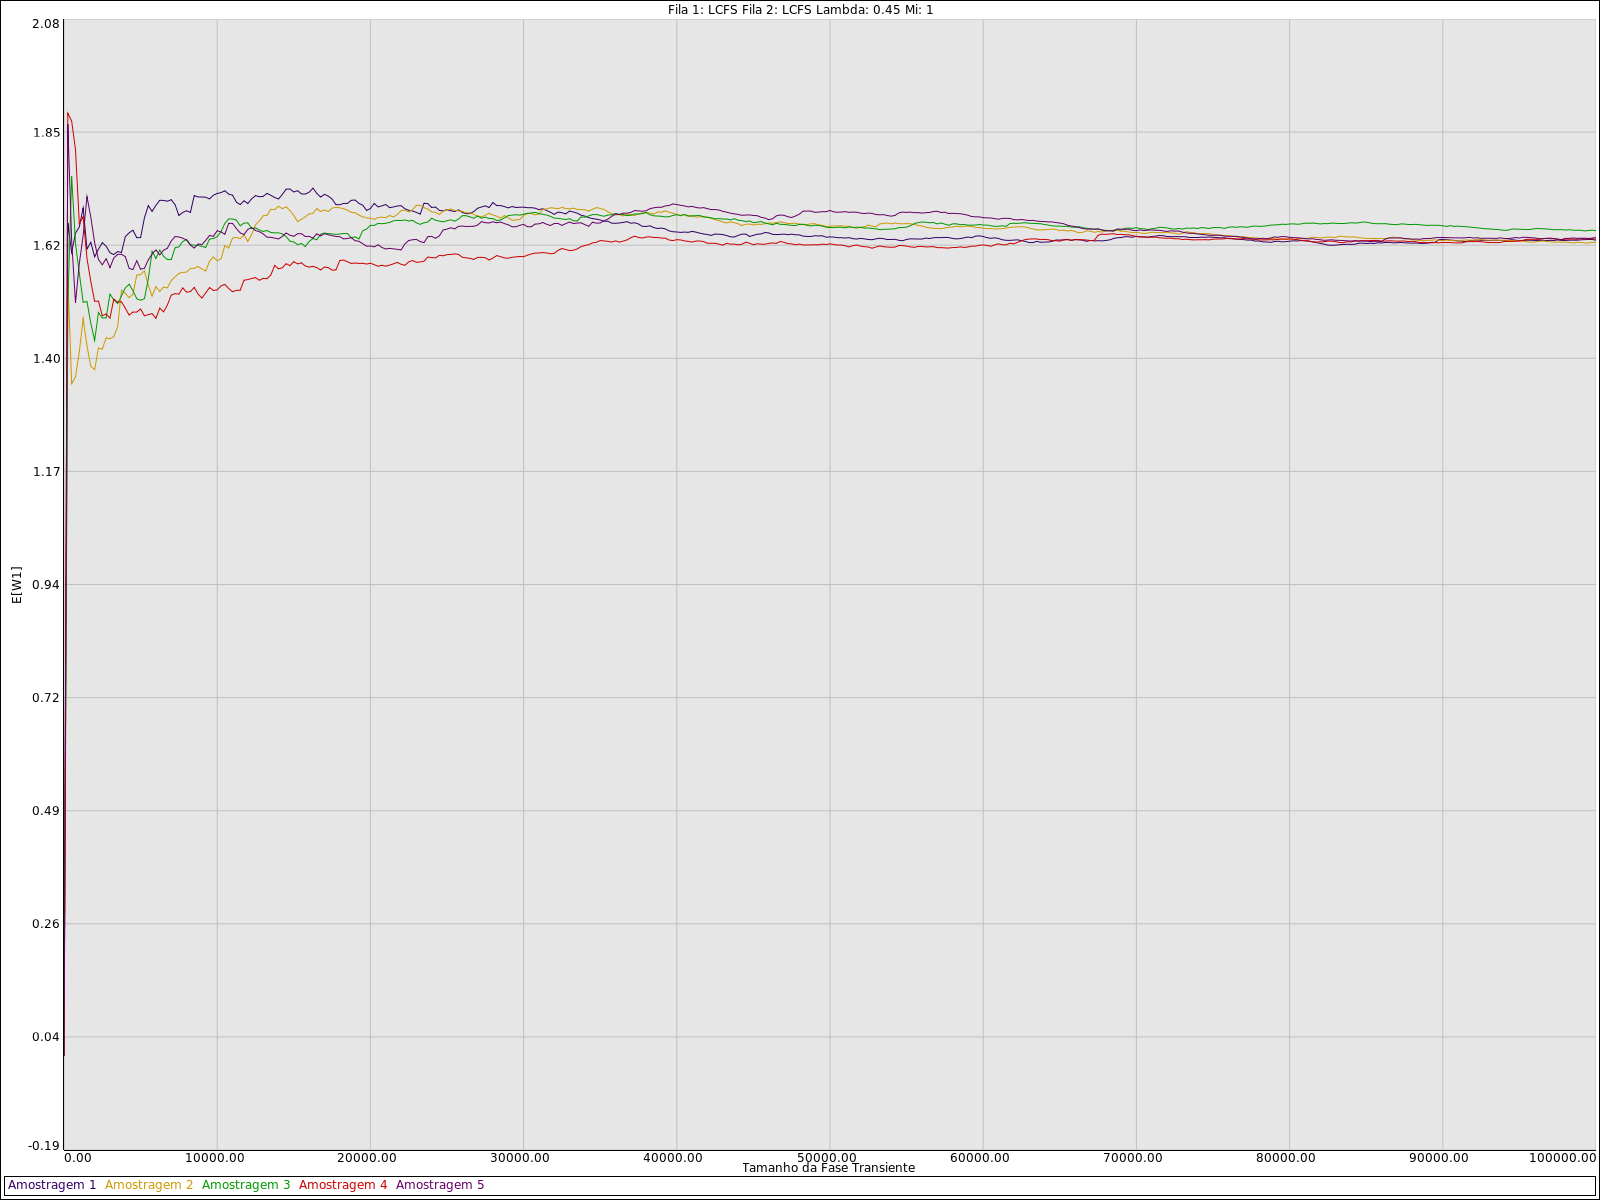
\includegraphics[scale = 0.20]{./graficos_transiente_1/LCFS/07.png}
\end{figure}

\begin{figure}
	\caption{Média da V.A. $W_2$, Serviço LCFS com $\lambda$ = 0.45}
	\label{figTransienteLCFSfila2W}
	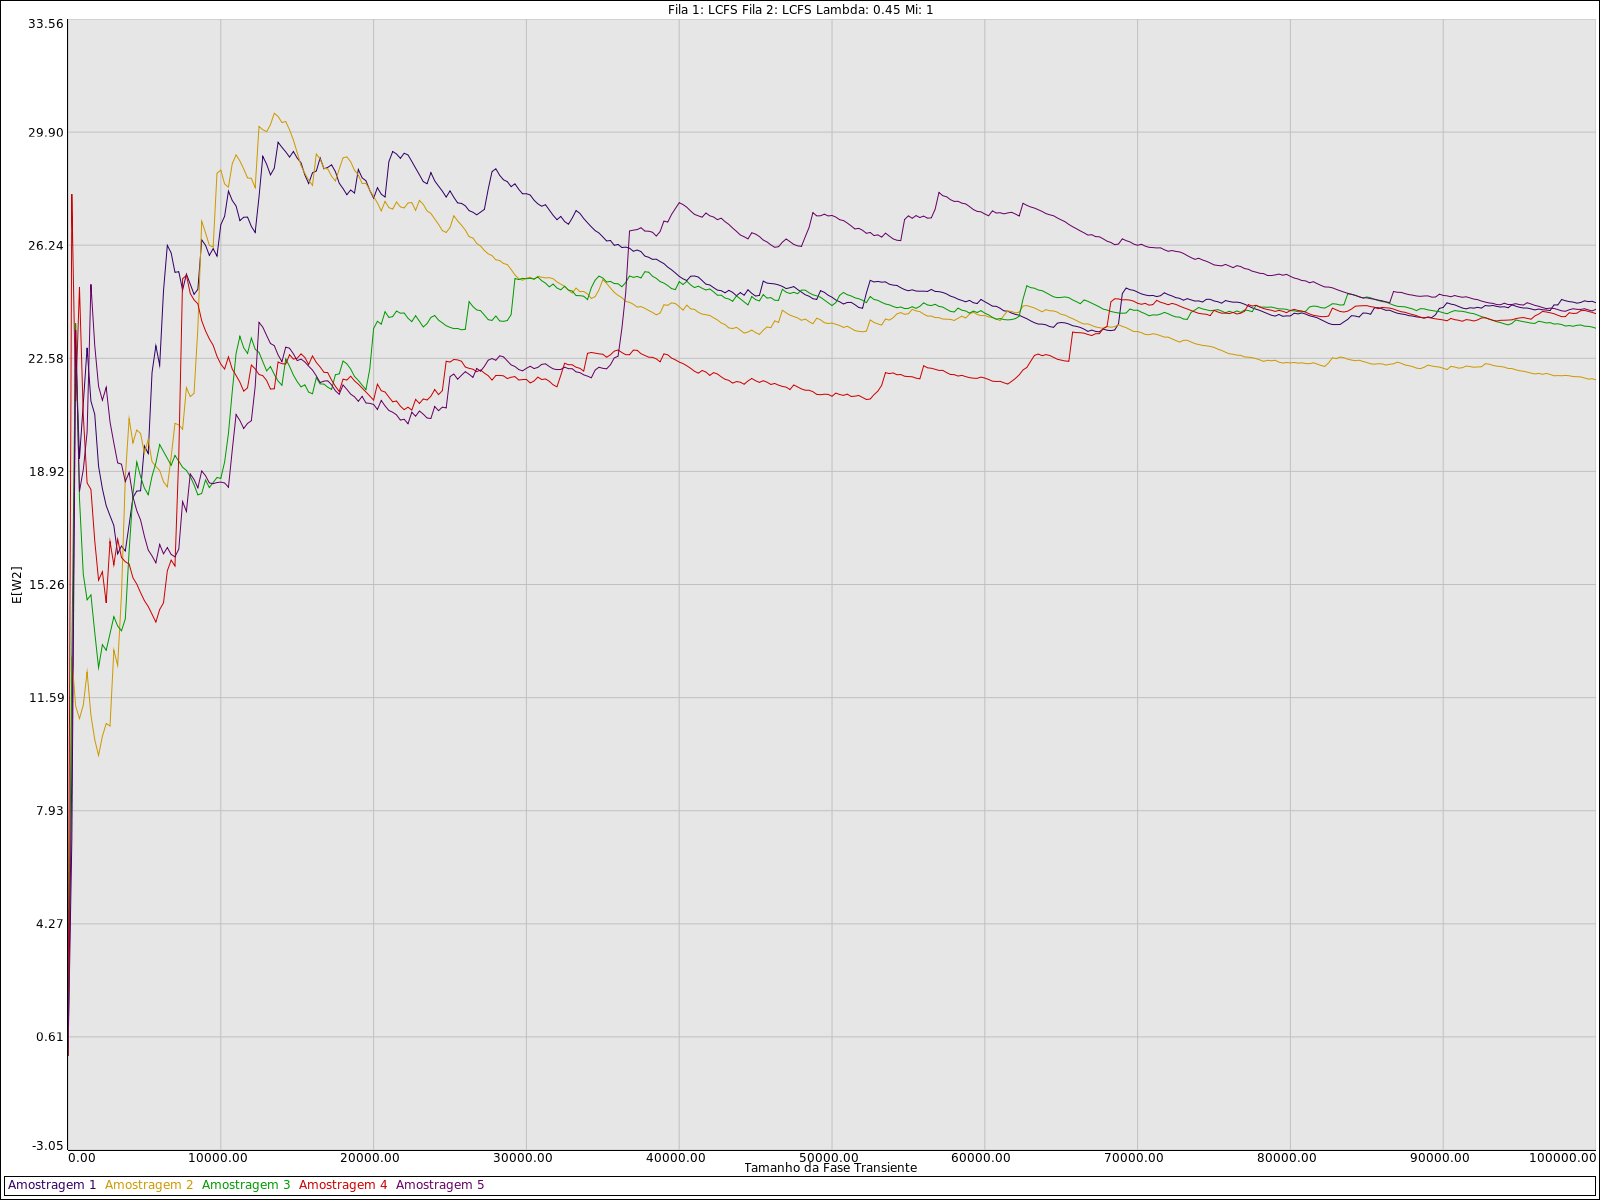
\includegraphics[scale = 0.20]{./graficos_transiente_1/LCFS/08.png}
\end{figure}

\begin{figure}
	\caption{Variância da V.A. $W_1$, Serviço LCFS com $\lambda$ = 0.45}
	\label{figTransienteLCFSfila1VarW}
	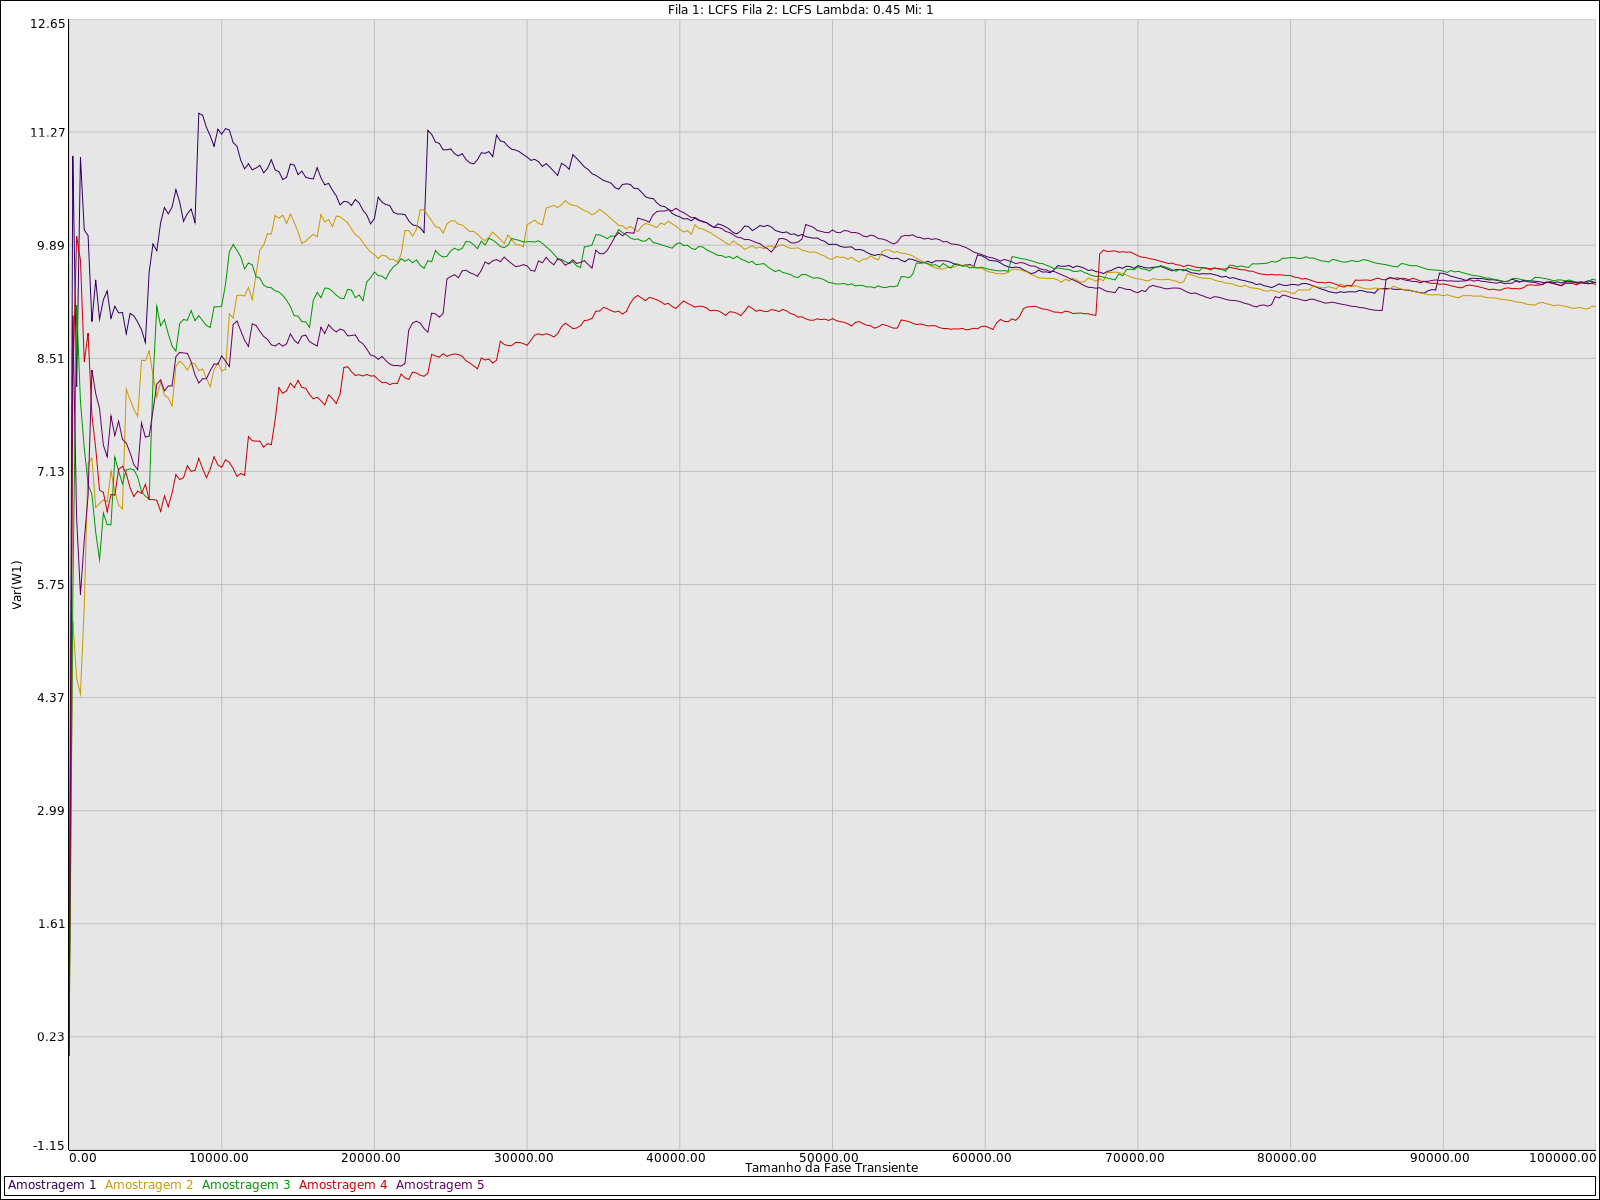
\includegraphics[scale = 0.20]{./graficos_transiente_1/LCFS/09.png}
\end{figure}

\begin{figure}
	\caption{Variância da V.A. $W_2$, Serviço LCFS com $\lambda$ = 0.45}
	\label{figTransienteLCFSfila2VarW}
	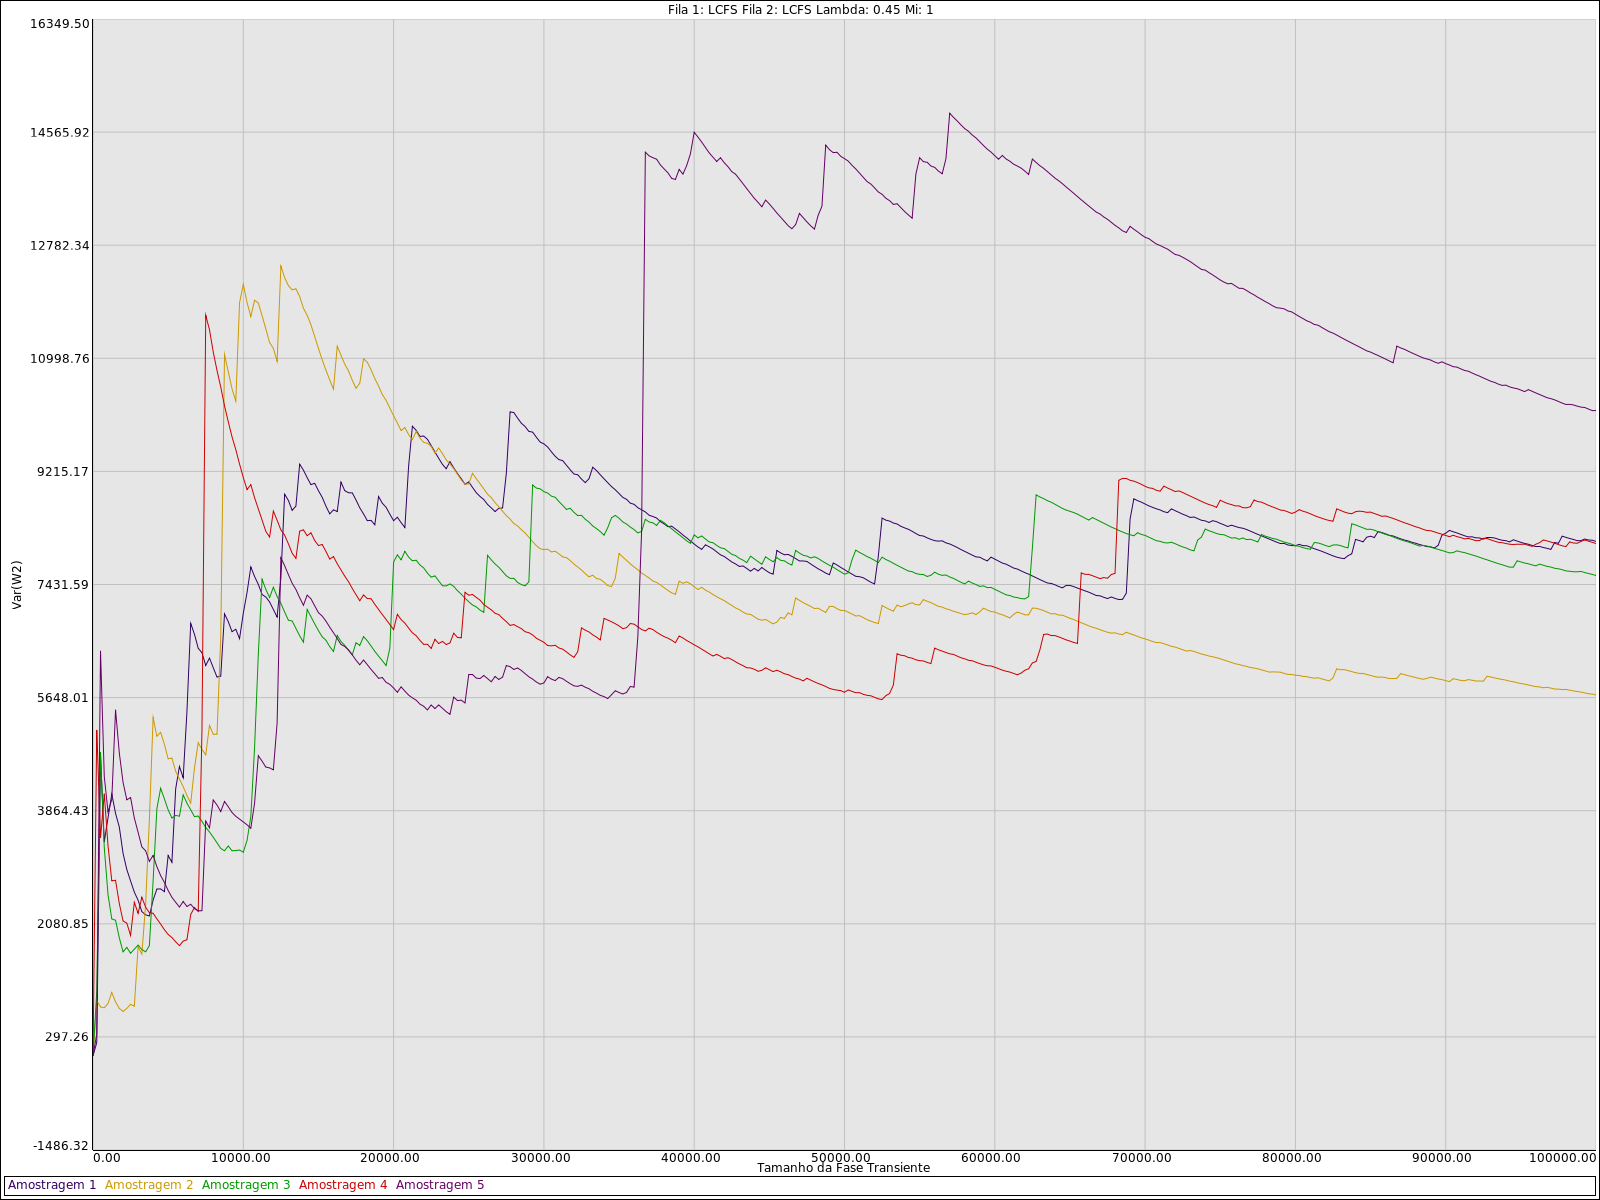
\includegraphics[scale = 0.20]{./graficos_transiente_1/LCFS/10.png}
\end{figure}

\clearpage

%figuras pra 10k de transiente
\begin{figure}
	\caption{Variância da V.A. $W_2$, Serviço FCFS com $\lambda$ = 0.10}
	\label{figTransienteFCFSfila2VarWLambda010}
	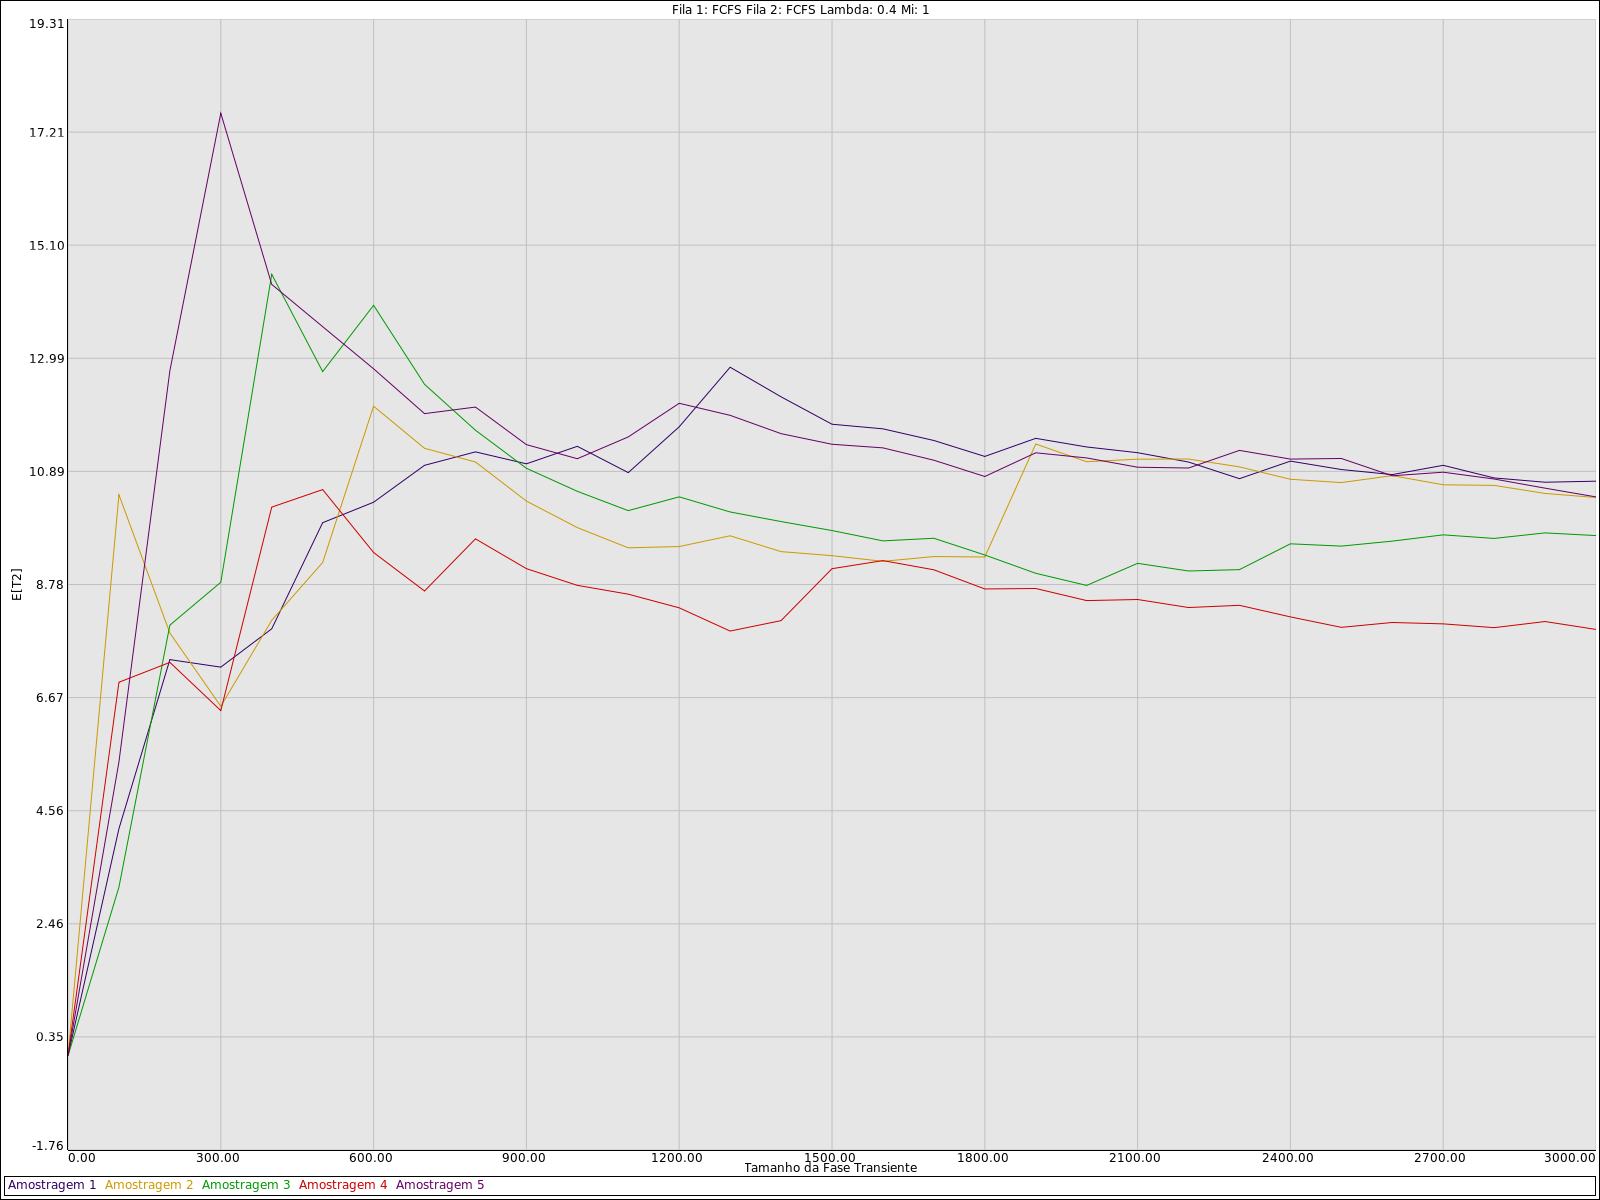
\includegraphics[scale = 0.20]{./graficos_transiente_2/01.png}
\end{figure}

\begin{figure}
	\caption{Variância da V.A. $W_2$, Serviço FCFS com $\lambda$ = 0.20}
	\label{figTransienteFCFSfila2VarWLambda020}
	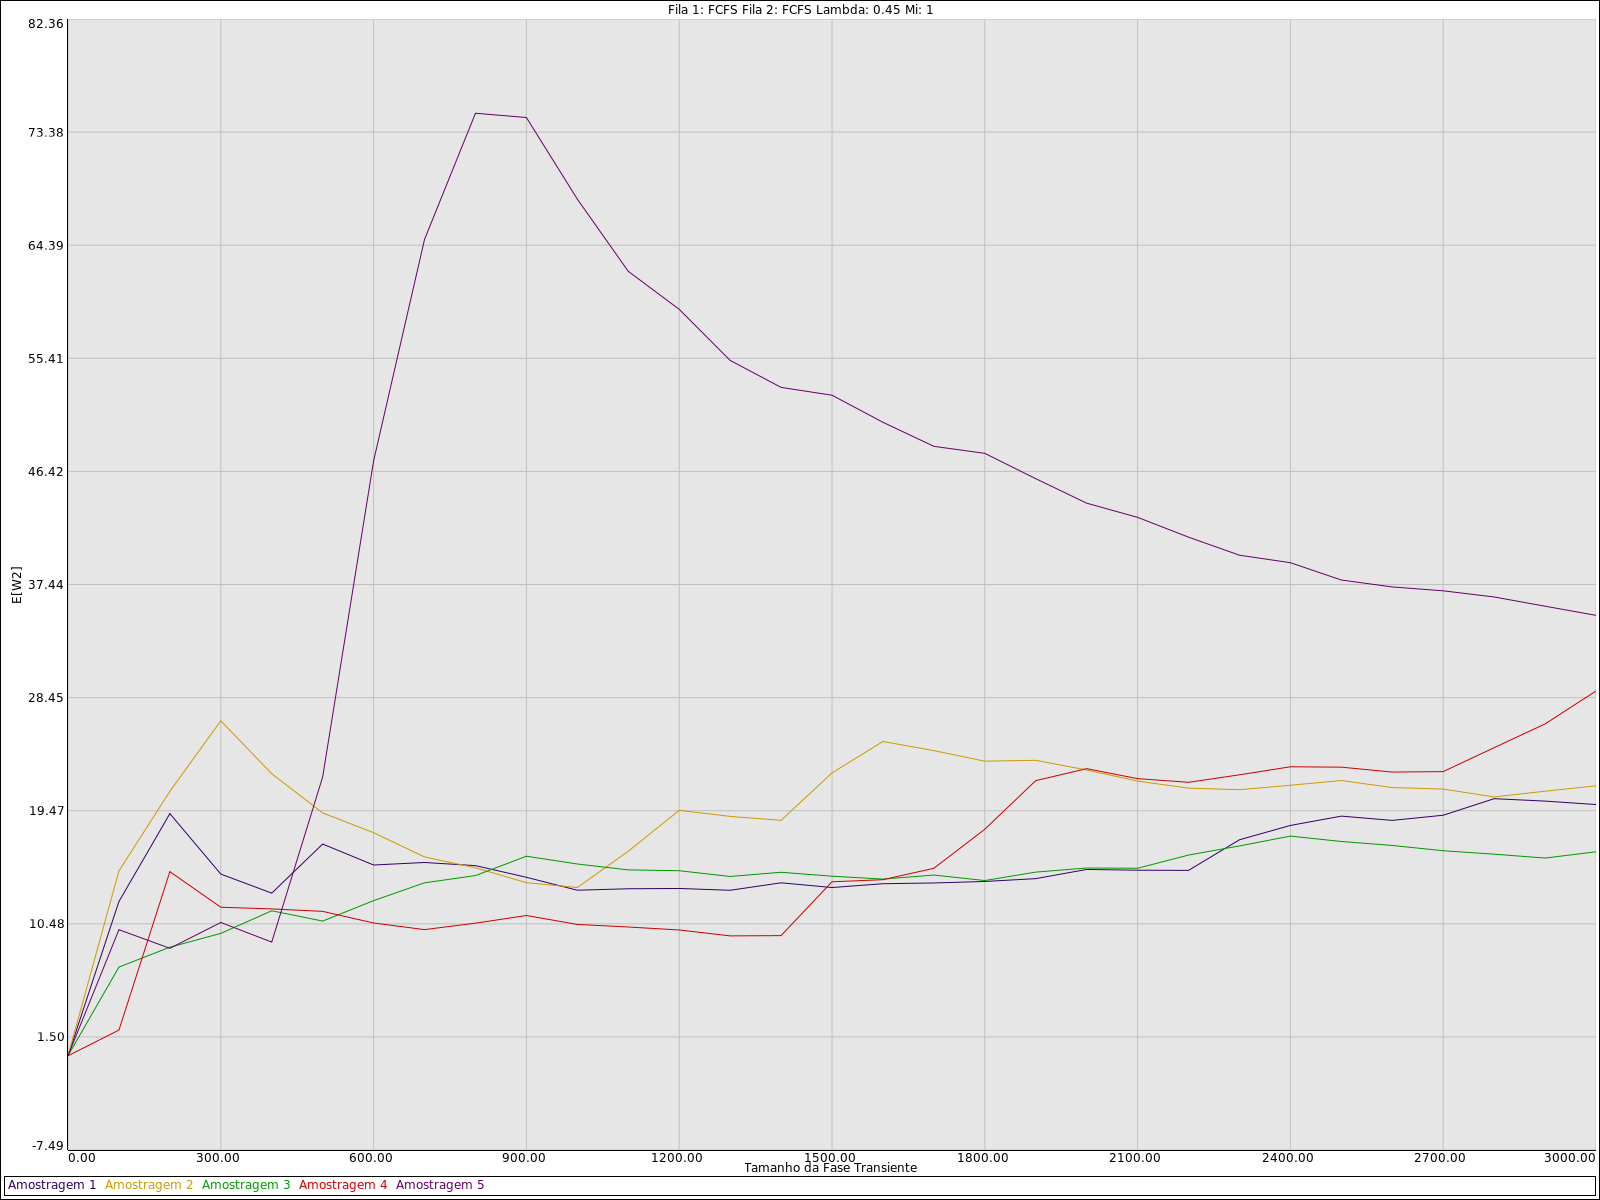
\includegraphics[scale = 0.20]{./graficos_transiente_2/02.png}
\end{figure}

\begin{figure}
	\caption{Variância da V.A. $W_2$, Serviço FCFS com $\lambda$ = 0.30}
	\label{figTransienteFCFSfila2VarWLambda030}
	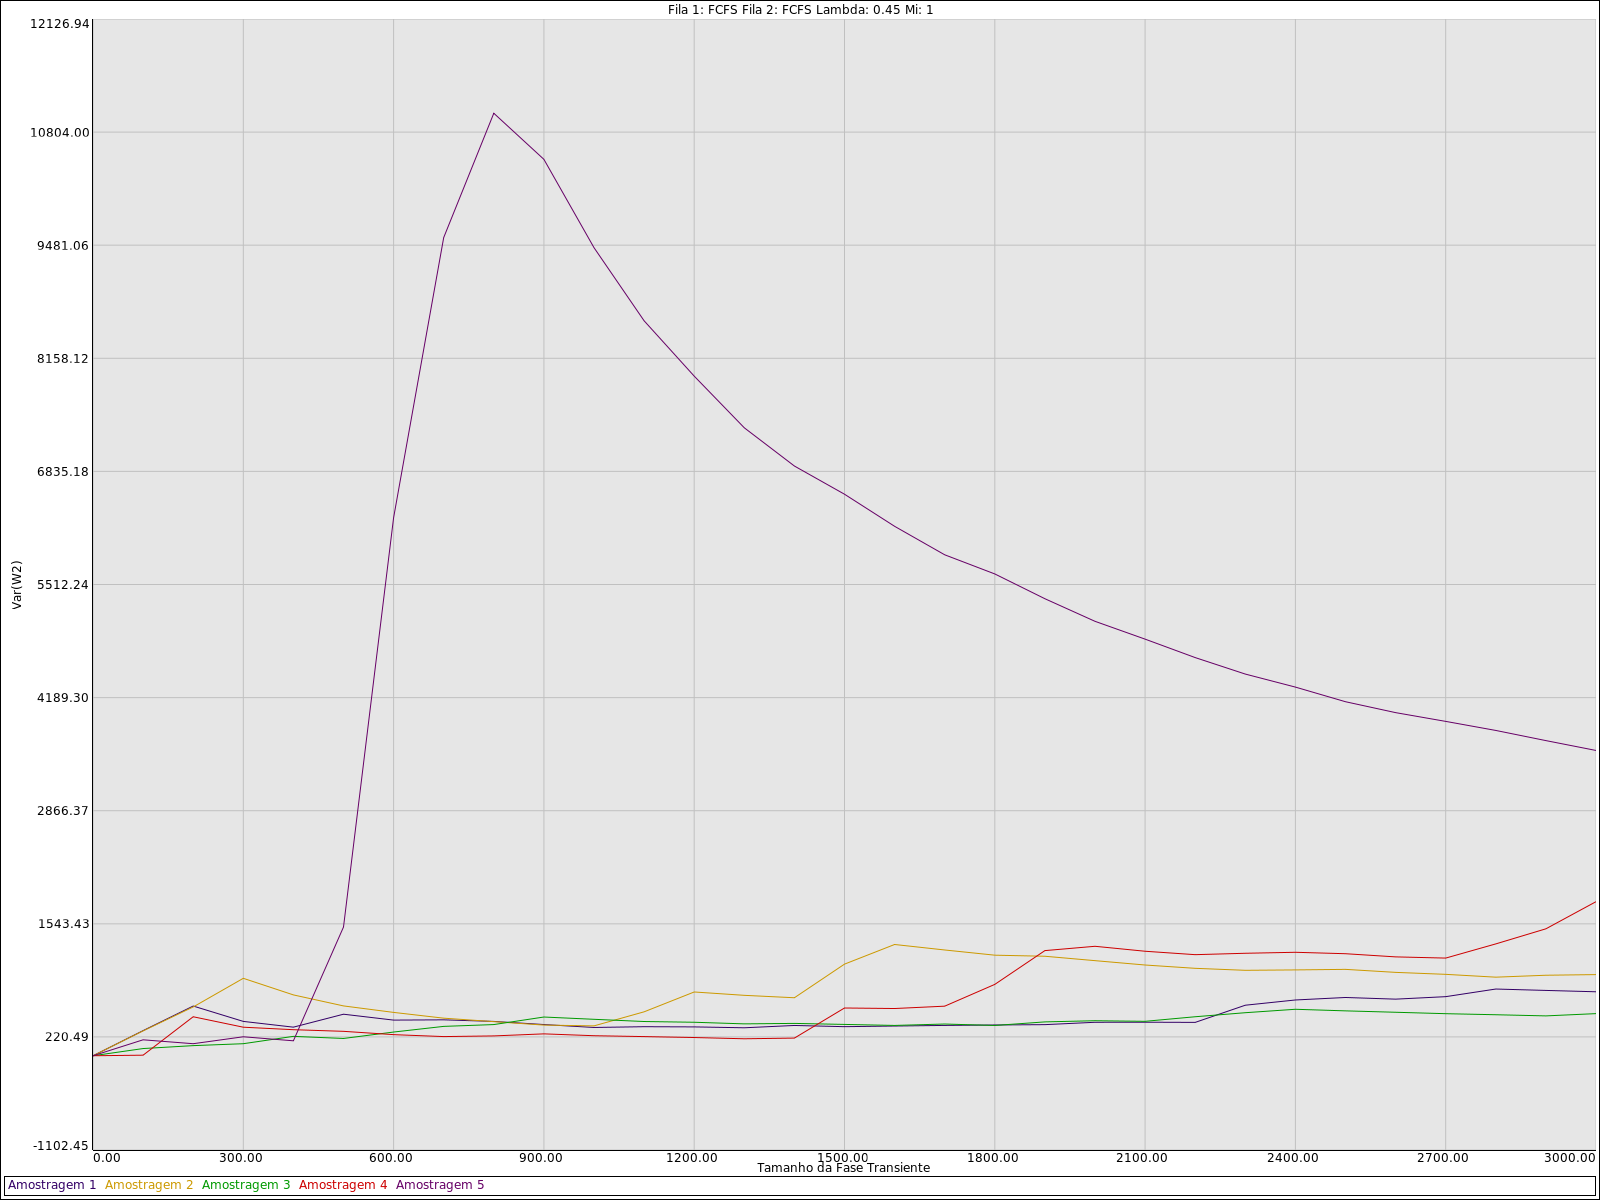
\includegraphics[scale = 0.20]{./graficos_transiente_2/03.png}
\end{figure}

\begin{figure}
	\caption{Variância da V.A. $W_2$, Serviço FCFS com $\lambda$ = 0.40}
	\label{figTransienteFCFSfila2VarWLambda040}
	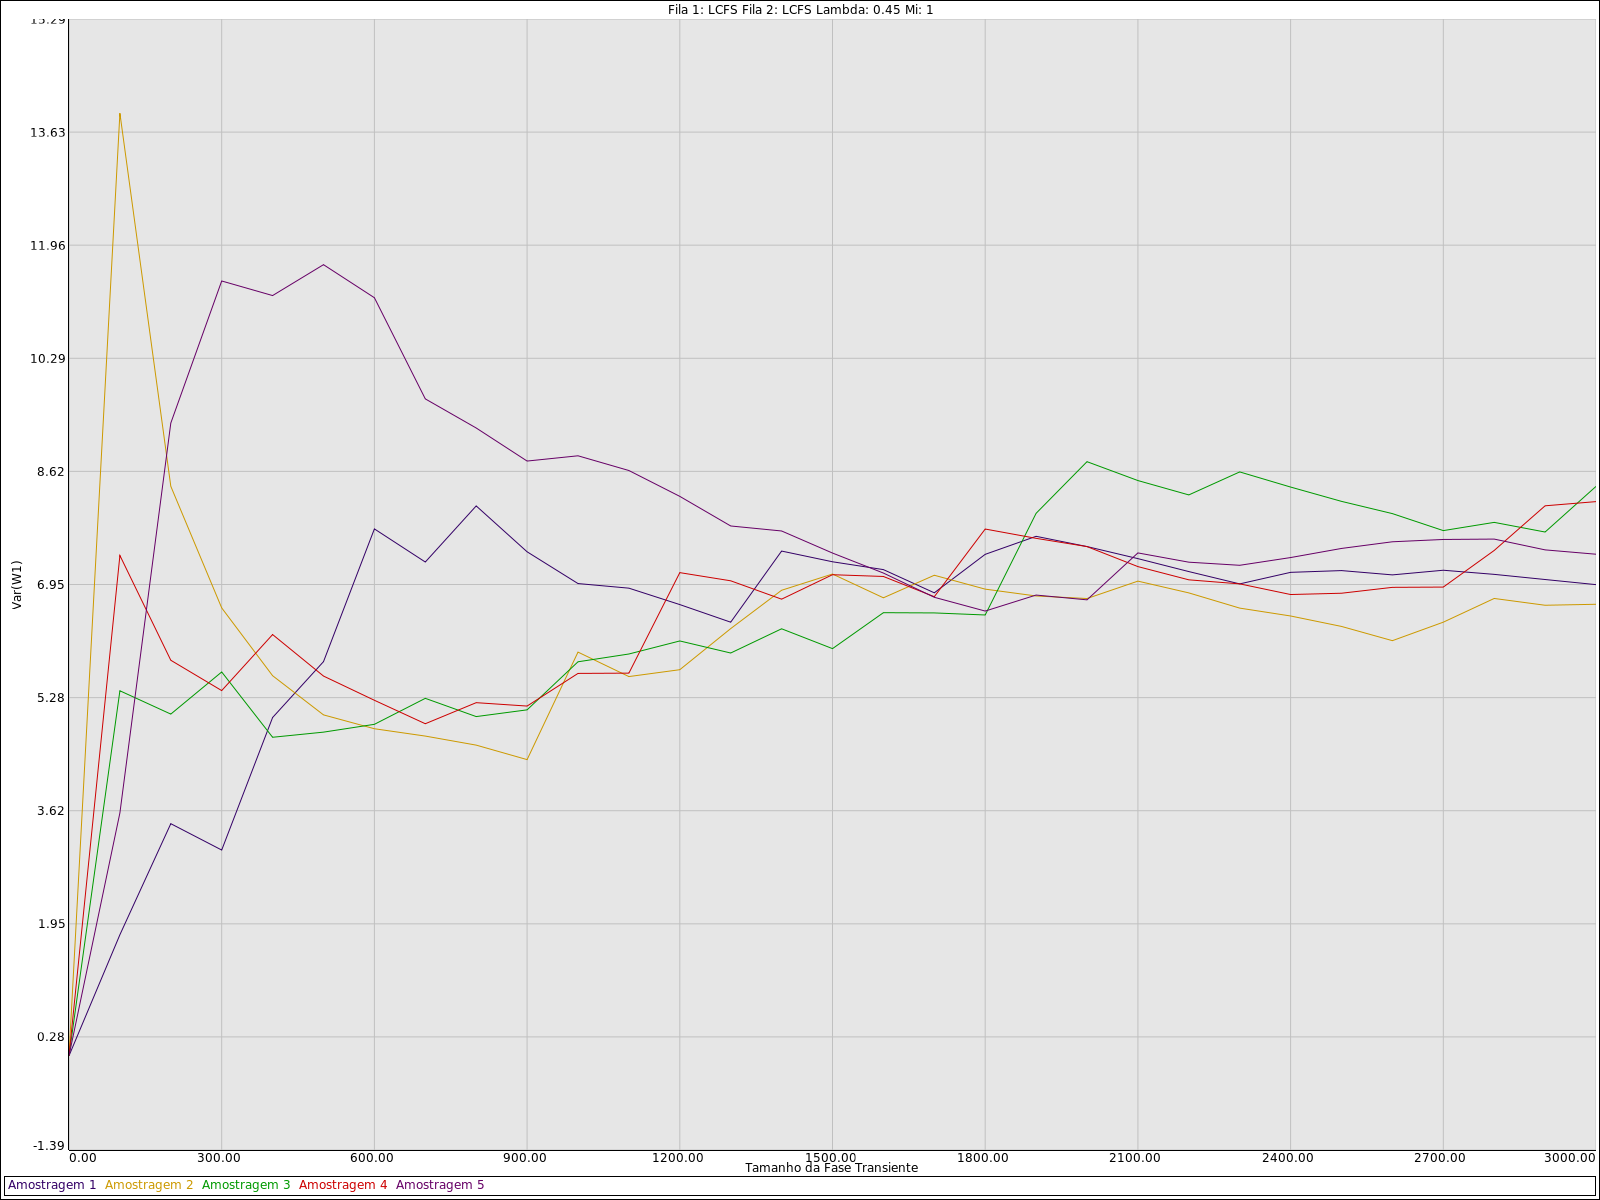
\includegraphics[scale = 0.20]{./graficos_transiente_2/04.png}
\end{figure}

\begin{figure}
	\caption{Variância da V.A. $W_2$, Serviço LCFS com $\lambda$ = 0.10}
	\label{figTransienteLCFSfila2VarWLambda010}
	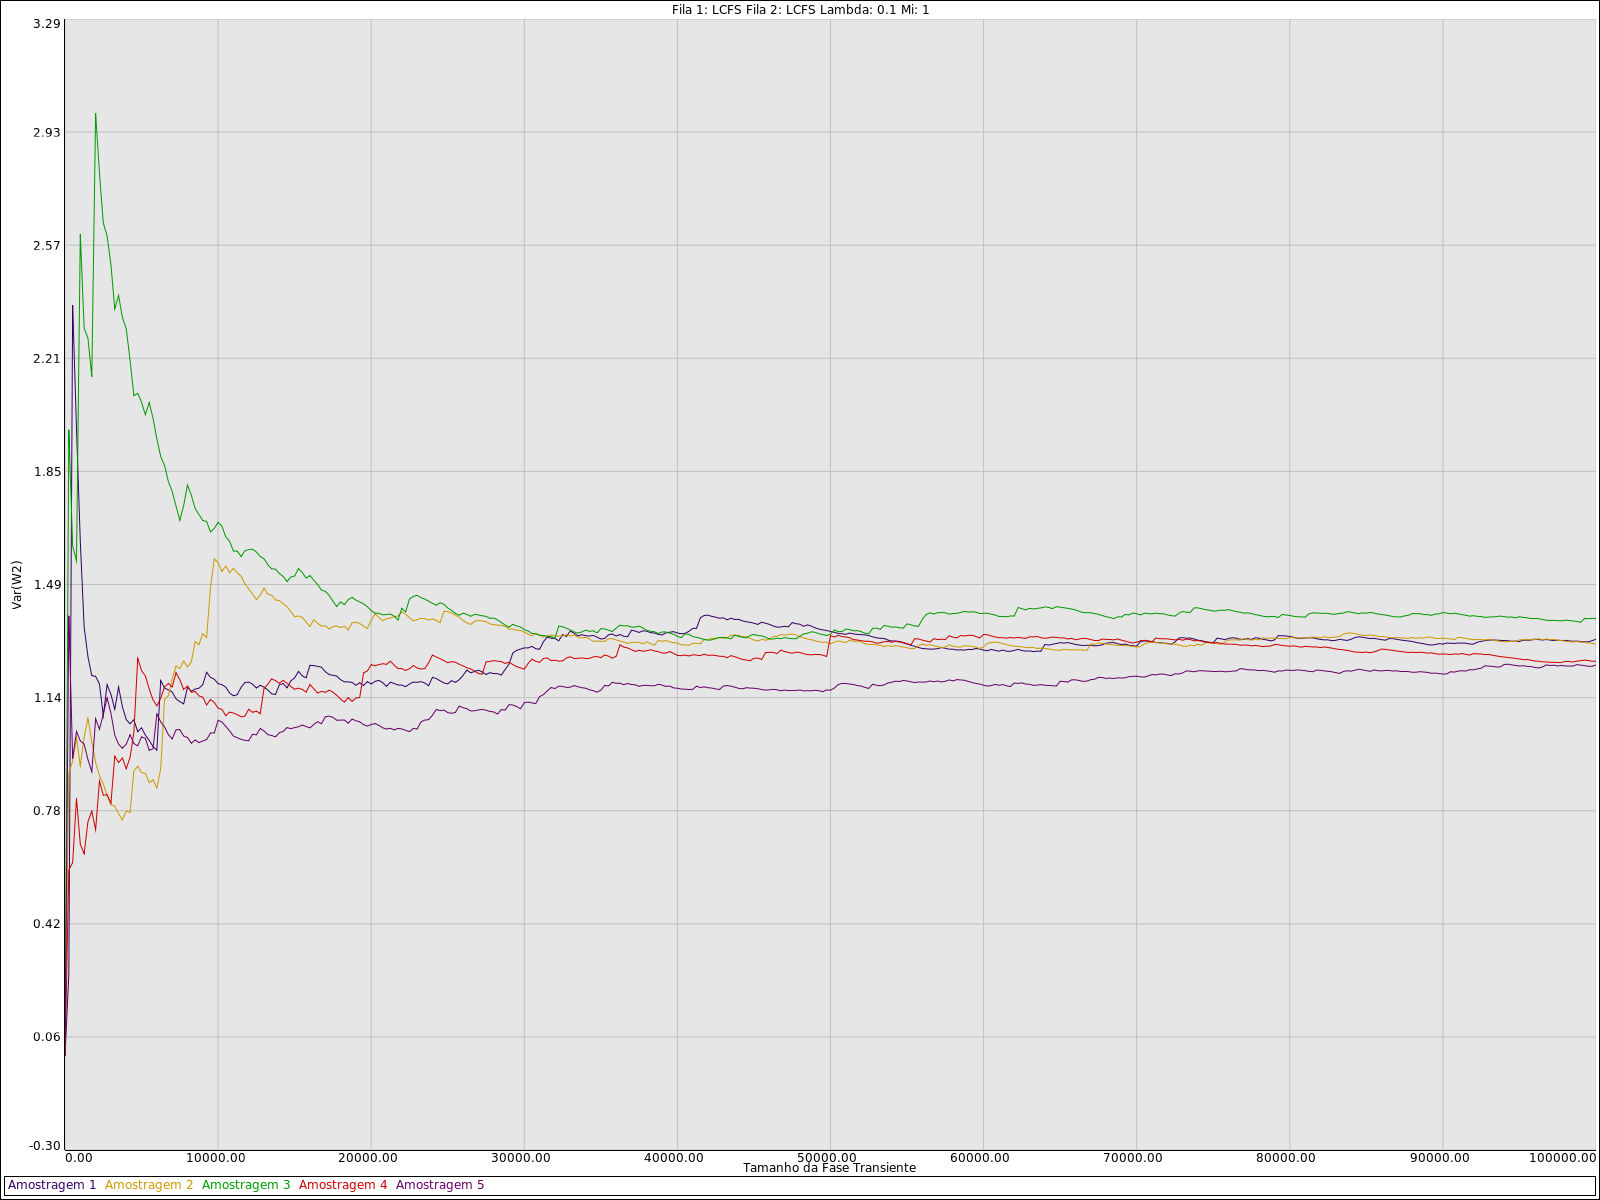
\includegraphics[scale = 0.20]{./graficos_transiente_2/05.png}
\end{figure}

\begin{figure}
	\caption{Variância da V.A. $W_2$, Serviço LCFS com $\lambda$ = 0.20}
	\label{figTransienteLCFSfila2VarWLambda020}
	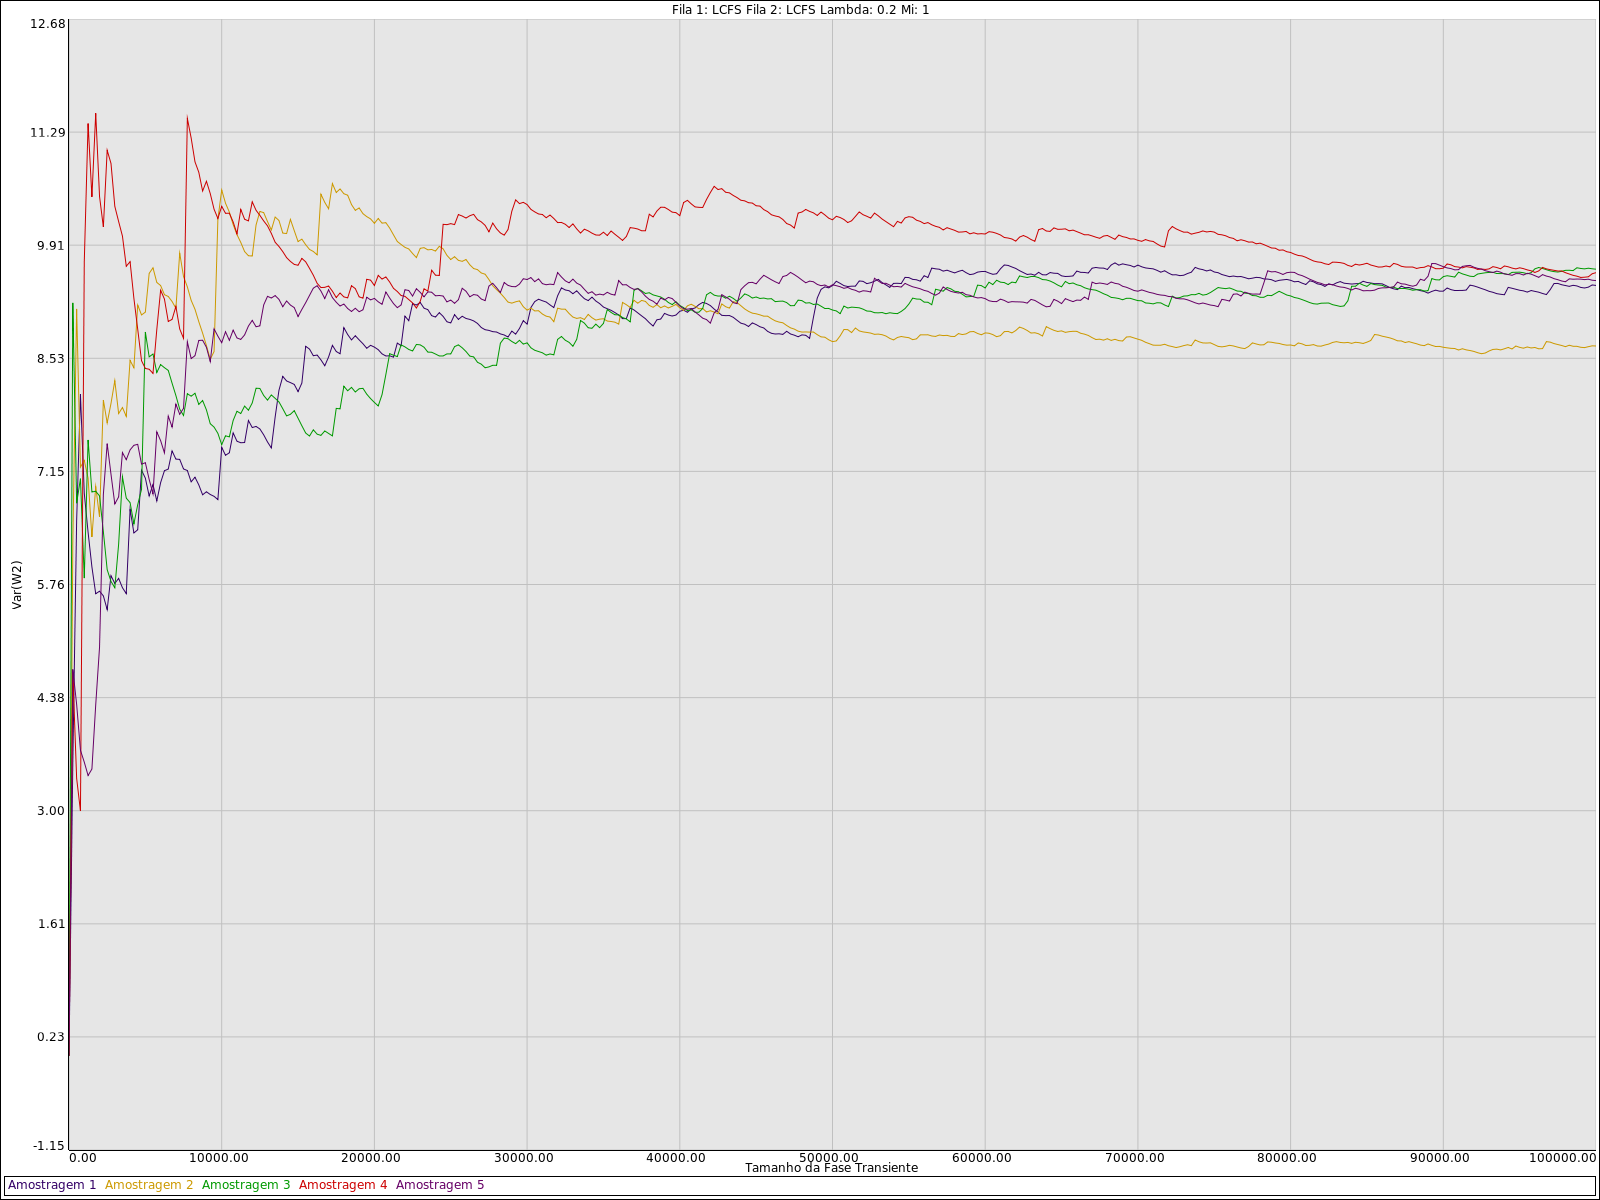
\includegraphics[scale = 0.20]{./graficos_transiente_2/06.png}
\end{figure}

\begin{figure}
	\caption{Variância da V.A. $W_2$, Serviço LCFS com $\lambda$ = 0.30}
	\label{figTransienteLCFSfila2VarWLambda030}
	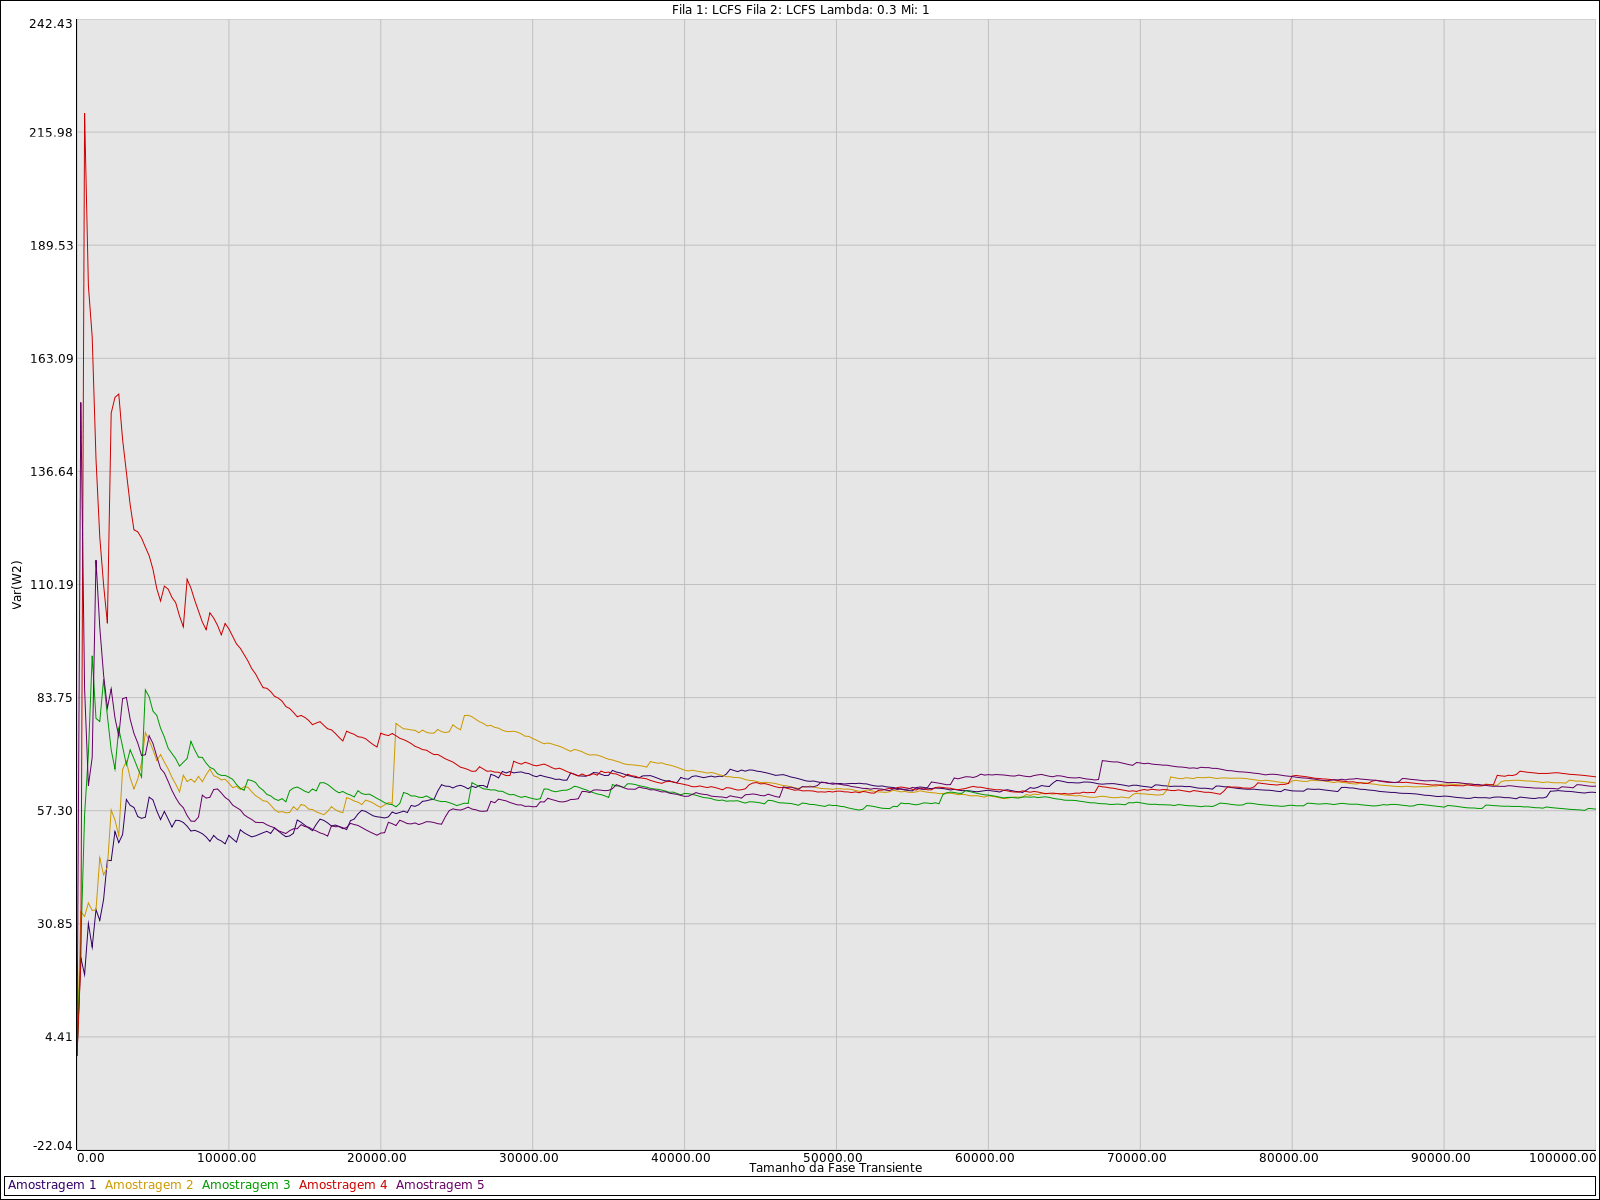
\includegraphics[scale = 0.20]{./graficos_transiente_2/07.png}
\end{figure}

\begin{figure}
	\caption{Variância da V.A. $W_2$, Serviço LCFS com $\lambda$ = 0.40}
	\label{figTransienteLCFSfila2VarWLambda040}
	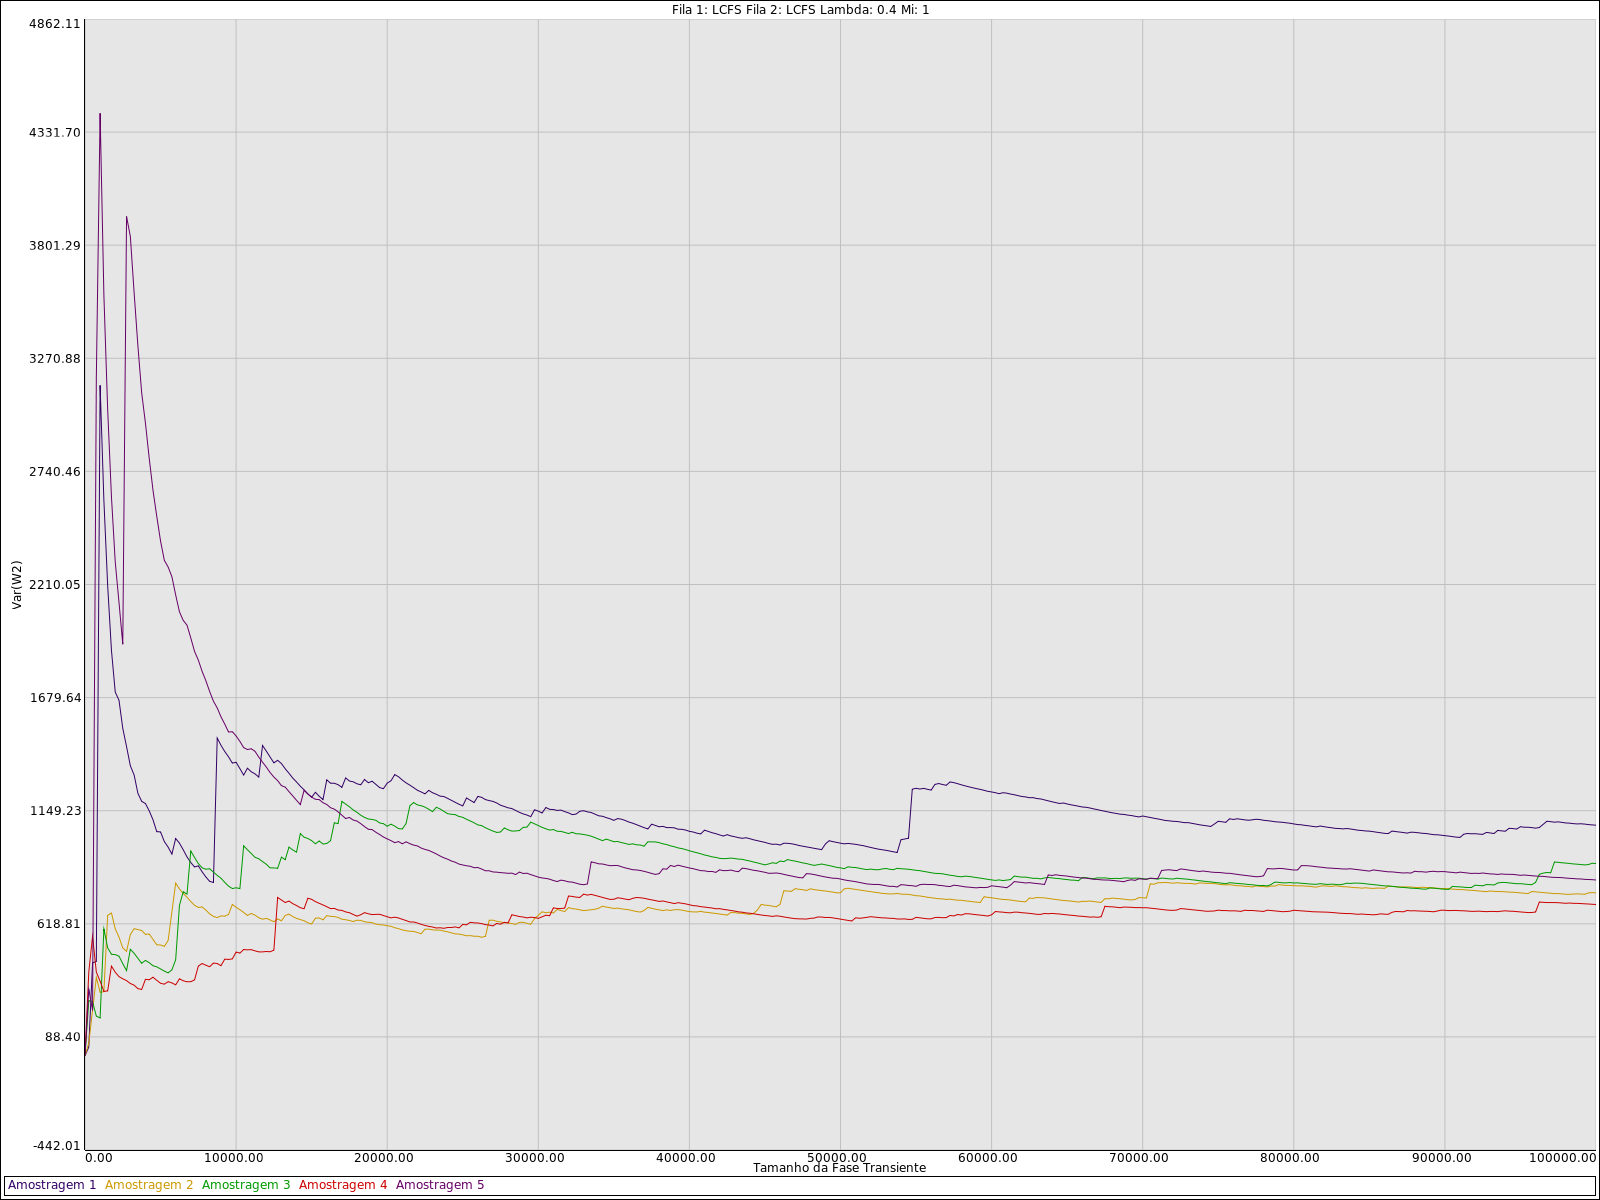
\includegraphics[scale = 0.20]{./graficos_transiente_2/08.png}
\end{figure}

\clearpage
\pagebreak

\section{Tabelas com resultados e comentários pertinentes}
% Tabelas, tabelas e tabelas. =)
\pagebreak

\section{Otimização}

    Para o cálculo dos fatores otimizados, o tamanho da fase transiente foi mantido o mesmo das simulações acima, ou seja, 10 mil para $\lambda = \{0.1, 0.2, 0.3, 0.4 \}$ e 50 mil para $\lambda = 0.45$. Como o modo de simulação escolhido para os testes foi o \emph{Batch}, a fase transiente acrescenta apenas uma valor constante à soma total.

Para o calculo do melhor fator possível, mas que ainda atendesse a restrição do tamanho dos intervalos de confiança, foi utilizado um programa adicional em Perl (também desenvolvido pelo grupo) que utiliza buscas binárias para encontrar o melhor fator entre o número de rodadas e o tamanho de cada rodada. O código fonte do programa esta no diretório \emph{scripts} e se chama \emph{otimização\_bb.pl}.

A metodologia para encontrar a fase transiente era:
\begin{enumerate}
	\item Encontrar um possível candidato;
	\item Realizar uma bateria de testes para garantir que os resultados do valor candidato sejam independentes da semente utilizada para inicializar os geradores do programa.
\end{enumerate}

    O grupo preferiu optar por uma margem segura, aceitando apenas candidatos nos quais todos os intervalos de confiança eram de tamanho menor ou igual a $8.5\%$ em relação à média da medida analisada. Talvez seja possível conseguir fatores menores ao utilizar margens menores como $9.0\%$ ou $9.5\%$, mas foi decidido, após diversos testes, que estas margens não eram confiáveis o suficiente para garantir os resultados independentes das sementes utilizadas.

Os resultados obtidos foram:

\begin{center}
\begin{tabular} { | c | c | c | c | c | r | }
    \hline
    Filas & $\lambda$  & Fase transiente  & Número de rodadas & Tamanho das rodadas  & FATOR \\ \hline
    FCFS     & $0.1$   & 10000 & 490     & 720      & 362800       \\ \hline
    FCFS     & $0.2$   & 10000 & 640     & 770      & 502800       \\ \hline
    FCFS     & $0.3$   & 10000 & 950     & 940      & 903000       \\ \hline
    FCFS     & $0.4$   & 10000 & 640     & 4100    & 2634000     \\ \hline
    FCFS     & $0.45$ & 50000 & 1110   & 8360    & 9329600     \\ \hline
    LCFS     & $0.1$   & 10000 & 320     & 1240    & 406800       \\ \hline
    LCFS     & $0.2$   & 10000 & 640     & 960      & 624400       \\ \hline
    LCFS     & $0.3$   & 10000 & 950     & 1260    & 1207000     \\ \hline
    LCFS     & $0.4$   & 10000 & 640     & 7300    & 4682000     \\ \hline
    LCFS     & $0.45$ & 50000 & 950     & 18700  & 17815000   \\ \hline
\end{tabular}
\end{center}


Cada resultado foi  posteriormente testado com mil sementes diferentes, em uma espécie de teste de estresse, sendo o resultado aprovado caso em $99.0\%$ ou mais das vezes nenhum intervalo de confiança fosse maior que $10\%$. O grupo chegou à conclusão que, se em no máximo 10 de 1000 simulações o tamanho do intervalo de confiança fosse um pouco maior que $10.0\%$, não seria necessário aumentar o fator. Foi considerado que esta abordagem teria um custo benefício muito baixo, dado a grande quantidade dos testes que passam dentro do limite com folga, pois a verificação inicial era de $8.5\%$ (relembrando: um fator candidato só era aprovado caso tivesse passado em 10 testes seguidos com todos os intervalos de confiança com tamanho menor ou igual a $8.5\%$).

Pudemos observar que devido à alta variância do tempo de espera na fila 2 quando esta opera em LCFS e com uma alta chegada no sistema($\lambda = 0.45$), o número necessário de amostras para um bom intervalo de confiança é bastante alto, o que já era esperado.

Uma curiosidade, foi que o otimizador ao trabalhar com $\lambda = 0.3$ sempre preferiu aumentar o número de rodadas do que aumentar o tamanho das mesmas. Ao prosseguir para $\lambda = 0.4$, o melhor fator foi encontrado reduzindo novamente o número de rodadas mas aumentando o tamanho de cada uma.

O tempo necessário para a execução do programa para o cálculo dos fatores otimizados para todos os casos foi de 2 horas e 30 minutos.

O tempo necessário para o teste de estresse foi por volta de 5 horas.

\pagebreak

\section{Conclusão}
%%Olhar coisas com a tag CONC%%

    Durante a realização do trabalho o grupo se deparou com alguns problemas, a maioria deles relacionados a parte não-determinística da simulação pois, ao utilizar uma semente inicial "ruim" para o(s) gerador(es) de números pseudo-aleatórios, os resultados do simulador algumas vezes geravam certa confusão, requerendo que o grupo implementasse uma grande e extensiva bateria de testes para ter mais confiança nos resultados obtidos.

Outra dificuldade foi a demonstração da corretude do simulador, mesmo em um sistema pequeno como este, pois normalmente não há uma abordagem clara e única para proceder.

    Sobre o software simulador implementado pelo grupo, consideramos que tem excelente nível, tanto em usabilidade quanto em implementação. Com uma boa velocidade e pequeno consumo de memória (devido a cuidados tomados no gerenciamento de memória, o que em C/C++ deve ser feito pelo próprio programador), o sistema apresenta uma ótima performance sendo possível, inclusive rodar nossos $stress tests$ em laptops com hardware já defasado para os padrões atuais.


    Uma melhora possível seria a inclusão da capacidade de $multi-threading$ para o modo Replicativo e para os programas em Perl que executam a bateria de testes. Pensando nisso, alguns cuidados foram tomados para facilitar a portabilidade do simulador para ambientes multi-thread como por exemplo a utilização da função \emph{drand48}, reentrante, como explicado na introdução deste relatório. Porém, devido as dificuldades já encontradas com o programa em single-thread, o grupo preferiu manter o código do simulador o mais simples possível, julgando que o tempo seria melhor gasto refinando o funcionamento e trabalhando na otimização do mesmo.

    Mesmo com um modo interativo, onde o software pergunta os parâmetros da simulação, uma interface gráfica para a utilização, apesar de não necessária, seria interessante. Outra idéia para a interface gráfica seriam a geração de gráficos simples em tempo real de execução do simulador, assim o usuário poderia acompanhar as medições feitas durante o processo de simulação. Apesar de não estar implementado, a maneira na qual o simulador foi estruturado permite que a confecção de tal interface seja plenamente possível, sem grandes mudanças no código.

    O grupo julgou de extrema importância o trabalho prático, não só para lidar com um ambiente de simulação em todos os seus detalhes, captura e análise de dados e geração de estatísticas mas, principalmente, para verificar na prática o aprendizado teórico adquirido na disciplina.
\pagebreak

\end{document}
